	%%%%%%%%%%%%%%%%%%%%%%%%%%%%%%%%%%%%%%%%%
% Thin Sectioned Essay
% LaTeX Template
% Version 1.0 (3/8/13)
%
% This template has been downloaded from:
% http://www.LaTeXTemplates.com
%
% Original Author:
% Nicolas Diaz (nsdiaz@uc.cl) with extensive modifications by:
% Vel (vel@latextemplates.com)
%
% License:
% CC BY-NC-SA 3.0 (http://creativecommons.org/licenses/by-nc-sa/3.0/)
%
%%%%%%%%%%%%%%%%%%%%%%%%%%%%%%%%%%%%%%%%%

%----------------------------------------------------------------------------------------
%	PACKAGES AND OTHER DOCUMENT CONFIGURATIONS
%----------------------------------------------------------------------------------------

\documentclass[a4paper, 11pt]{article} % Font size (can be 10pt, 11pt or 12pt) and paper size (remove a4paper for US letter paper)

\usepackage[toc,page]{appendix}

\usepackage{tikz}

\usepackage{mathtools}
\usepackage[utf8x]{inputenc}

\usepackage{url}
\usepackage{amsmath}
\usepackage{hyperref}
\usepackage{listings}
\usepackage{subcaption}

\usetikzlibrary{arrows, patterns, calc, decorations.pathreplacing, shapes, plotmarks}

\usepackage{amsmath}
\usepackage[protrusion=true,expansion=true]{microtype} % Better typography
\usepackage{graphicx} % Required for including pictures
\usepackage{wrapfig} % Allows in-line images

\usepackage{mathpazo} % Use the Palatino font
\usepackage[T1]{fontenc} % Required for accented characters
\linespread{1.05} % Change line spacing here, Palatino benefits from a slight increase by default

\makeatletter
\renewcommand\@biblabel[1]{\textbf{#1.}} % Change the square brackets for each bibliography item from '[1]' to '1.'
\renewcommand{\@listI}{\itemsep=0pt} % Reduce the space between items in the itemize and enumerate environments and the bibliography

\renewcommand{\contentsname}{Indice} % Rename TOC default title

\renewcommand{\maketitle}{ % Customize the title - do not edit title and author name here, see the TITLE block below
\begin{flushright} % Right align
{\LARGE\@title} % Increase the font size of the title

\vspace{50pt} % Some vertical space between the title and author name

{\large\@author} % Author name
\\\@date % Date

\vspace{40pt} % Some vertical space between the author block and abstract
\end{flushright}
}

%\setcounter{tocdepth}{5}
\usepackage{hyperref} % Enables hyperlinking (e.g., ToC)

%----------------------------------------------------------------------------------------
%	TITLE
%----------------------------------------------------------------------------------------

\title{\textbf{MrsP}\\ % Title
\vspace{10pt}Capitolo esperimenti e valutazione} % Subtitle

\author{\textsc{Sebastiano Catellani} % Author
\vspace{20pt}\\{\textit{Universita' degli Studi di Padova}}} % Institution

\date{\today} % Date

%----------------------------------------------------------------------------------------

%%%%%%%%%%%%%%%%% SCHED MIN %%%%%%%%%%%%%%%%%%%%%%%
\begin{filecontents}{PFPschedMIN.data}
#Utilization   Times $\mu$s
1.0  16.85
2.0  17.60
3.0  16.63
3.5  15.54
4.0  16.29
4.5  16.16
5.0  15.96
6.0  15.87
\end{filecontents}

\begin{filecontents}{MRSPschedMIN.data}
#Utilization   Times $\mu$s
1.0  15.20
2.0  17.88
3.0  15.72
3.5  14.34
4.0  15.53
4.5  14.28
5.0  14.56
6.0  14.32
\end{filecontents}
%%%%%%%%%%%%%%%%%%%%%%%%%%%%%%%%%%%%%%%%%%%%%%%%%%%

%%%%%%%%%%%%%%%%% SCHED MAX %%%%%%%%%%%%%%%%%%%%%%%
\begin{filecontents}{PFPschedMAX.data}
#Utilization   Times $\mu$s
1.0  3.1108
2.0  5.1018
3.0  4.8526
3.5  3.1108
4.0  4.2522
4.5  2.9623
5.0  3.7787
6.0  2.8438
\end{filecontents}

\begin{filecontents}{MRSPschedMAX.data}
#Utilization   Times $\mu$s
1.0  2.8438
2.0  5.1799
3.0  4.8708
3.5  3.6047
4.0  4.3150
4.5  2.9238
5.0  3.4238
6.0  2.8985
\end{filecontents}
%%%%%%%%%%%%%%%%%%%%%%%%%%%%%%%%%%%%%%%%%%%%%%%%%%%

%%%%%%%%%%%%%%%%% SCHED AVG %%%%%%%%%%%%%%%%%%%%%%%
\begin{filecontents}{PFPschedAVG.data}
#Utilization   Times $\mu$s
1.0  17.554
2.0  14.035
3.0  12.020
3.5  9.862
4.0  10.253
4.5  8.302
5.0  9.532
6.0  7.846
\end{filecontents}

\begin{filecontents}{MRSPschedAVG.data}
#Utilization   Times $\mu$s
1.0  16.085
2.0  13.076
3.0  11.795
3.5  10.968
4.0  10.374
4.5  9.009
5.0  9.392
6.0  8.349
\end{filecontents}
%%%%%%%%%%%%%%%%%%%%%%%%%%%%%%%%%%%%%%%%%%%%%%%%%%%

%%%%%%%%%%%%%%%%%%%%%%%%%%%%%%%%%%%%%%%%%%%%%%%%%%%
%%%%%%%%%%%%%%%%%%%%%%%%%%%%%%%%%%%%%%%%%%%%%%%%%%%

%%%%%%%%%%%%%%%%% RELEASE MIN %%%%%%%%%%%%%%%%%%%%%%%
\begin{filecontents}{PFPreleaseMIN.data}
#Utilization   Times $\mu$s
1.0  14.27
2.0  14.36
3.0  12.54
3.5  12.82
4.0  12.13
4.5  12.95
5.0  12.65
6.0  12.40
\end{filecontents}

\begin{filecontents}{MRSPreleaseMIN.data}
#Utilization   Times $\mu$s
1.0  12.84
2.0  12.90
3.0  11.86
3.5  11.36
4.0  11.84
4.5  11.70
5.0  12.04
6.0  11.74
\end{filecontents}

%%%%%%%%%%%%%%%%%%%%%%%%%%%%%%%%%%%%%%%%%%%%%%%%%%%

%%%%%%%%%%%%%%%%% RELEASE MAX %%%%%%%%%%%%%%%%%%%%%%%
\begin{filecontents}{PFPreleaseMAX.data}
#Utilization   Times $\mu$s
1.0  2.2583
2.0  2.2429
3.0  2.3804
3.5  2.2704
4.0  2.3694
4.5  2.3535
5.0  2.3551
6.0  1.8062
\end{filecontents}

\begin{filecontents}{MRSPreleaseMAX.data}
#Utilization   Times $\mu$s
1.0  2.3584
2.0  2.1505
3.0  2.0218
3.5  1.8102
4.0  1.8348
4.5  1.7323
5.0  1.7652
6.0  1.2591
\end{filecontents}
%%%%%%%%%%%%%%%%%%%%%%%%%%%%%%%%%%%%%%%%%%%%%%%%%%%

%%%%%%%%%%%%%%%%% RELEASE AVG %%%%%%%%%%%%%%%%%%%%%%%
\begin{filecontents}{PFPreleaseAVG.data}
#Utilization   Times $\mu$s
1.0  9.110
2.0  7.980
3.0  7.291
3.5  6.390
4.0  6.634
4.5  5.420
5.0  5.751
6.0  4.366
\end{filecontents}

\begin{filecontents}{MRSPreleaseAVG.data}
#Utilization   Times $\mu$s
1.0  7.960
2.0  6.726
3.0  6.072
3.5  5.396
4.0  4.833
4.5  4.276
5.0  3.951
6.0  3.542
\end{filecontents}
%%%%%%%%%%%%%%%%%%%%%%%%%%%%%%%%%%%%%%%%%%%%%%%%%%%

%%%%%%%%%%%%%%%%%%%%%%%%%%%%%%%%%%%%%%%%%%%%%%%%%%%
%%%%%%%%%%%%%%%%%%%%%%%%%%%%%%%%%%%%%%%%%%%%%%%%%%%

%%%%%%%%%%%%%%%%% CXS MIN %%%%%%%%%%%%%%%%%%%%%%%
\begin{filecontents}{PFPcxsMIN.data}
#Utilization   Times $\mu$s
1.0  15.37
2.0  14.27
3.0  15.52
3.5  13.23
4.0  12.13
4.5  11.82
5.0  12.83
6.0  12.79
\end{filecontents}

\begin{filecontents}{MRSPcxsMIN.data}
#Utilization   Times $\mu$s
1.0  15.38
2.0  15.68
3.0  15.76
3.5  13.67
4.0  13.17
4.5  12.51
5.0  13.74
6.0  14.30
\end{filecontents}

%%%%%%%%%%%%%%%%%%%%%%%%%%%%%%%%%%%%%%%%%%%%%%%%%%%

%%%%%%%%%%%%%%%%% CXS MAX %%%%%%%%%%%%%%%%%%%%%%%
\begin{filecontents}{PFPcxsMAX.data}
#Utilization   Times $\mu$s
1.0  5.1078
2.0  4.2270
3.0  3.7190
3.5  3.1229
4.0  3.0994
4.5  2.7984
5.0  2.4619
6.0  1.9890
\end{filecontents}

\begin{filecontents}{MRSPcxsMAX.data}
#Utilization   Times $\mu$s
1.0  4.8754
2.0  3.6499
3.0  3.8999
3.5  3.7151
4.0  2.9622
4.5  2.8777
5.0  1.9098
6.0  1.4922
\end{filecontents}
%%%%%%%%%%%%%%%%%%%%%%%%%%%%%%%%%%%%%%%%%%%%%%%%%%%

%%%%%%%%%%%%%%%%% CXS AVG %%%%%%%%%%%%%%%%%%%%%%%
\begin{filecontents}{PFPcxsAVG.data}
#Utilization   Times $\mu$s
1.0  10.019
2.0  8.022
3.0  6.677
3.5  4.931
4.0  5.067
4.5  3.870
5.0  4.233 
6.0  3.219
\end{filecontents}

\begin{filecontents}{MRSPcxsAVG.data}
#Utilization   Times $\mu$s
1.0  8.759
2.0  6.620
3.0  5.528
3.5  4.825
4.0  4.267
4.5  3.573
5.0  3.323
6.0  2.885
\end{filecontents}
%%%%%%%%%%%%%%%%%%%%%%%%%%%%%%%%%%%%%%%%%%%%%%%%%%%

\begin{document}

\maketitle % Print the title section

\newpage

\tableofcontents % Print the Table of Contents

\newpage

\newcommand{\model}{%
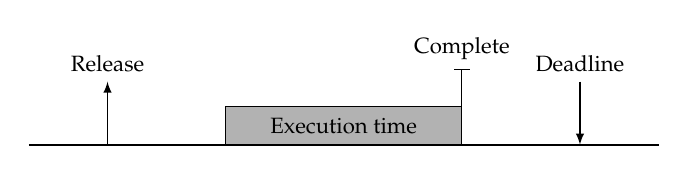
\begin{tikzpicture}[
  yscale = 0.8,
  normal/.style={fill=black!30},
  release/.style={-latex},
  complet/.style={-|},
  every text node part/.style={align=center}
]
%general params
\def\th{.6} %task height
\def\blockdim{(.4,.4)}
\def\arrowdim{(0,.5)}
\def\arrowdimB{(0,.4)}

%axes
\draw[thick, black] (0,0) -- (8, 0);

%L1
\draw[release] (1, 0) -- +(0,1) node[above] {{\footnotesize Release}};
\draw[normal]  (2.5, 0) rectangle +(3, \th) node[midway] {{\footnotesize Execution time}};
\draw[complet] (5.5, 0) -- +(0, 1.2) node[above] {{\footnotesize Complete}};
\draw[release] (7, 1) node[above] {{\footnotesize Deadline}} -- (7,0);

\end{tikzpicture}
}

\newcommand{\smallqueue}[2]{%
\draw[queuesty] (#1)node[right,xshift=.1cm]{\sffamily #2}-- ++(.2,.15)-- ++(.8,0)-- ++(0,-.3)-- ++(-.8,0)-- cycle;}
\newcommand{\bigqueue}[2]{%
\draw[queuesty] (#1)node[right,xshift=.2cm]{\sffamily #2}-- ++(.3,.3)-- ++(.8,0)-- ++(0,-.6)-- ++(-.8,0)-- cycle;}

\newcommand{\MrsP}[2]{%
\begin{tikzpicture}[
  xscale=#1,
  yscale=#2,
  every node/.append style={transform shape},
  queuesty/.style={fill=white, very thick, font=\tiny},
  cpusty/.style={fill=gray!40, draw, circle, minimum width=1cm},
  srpsty/.style={fill=white, draw, circle, text width=.17cm, font=\tiny, very thick},
  ressty/.style={fill=red!30, draw, very thick, rounded corners=5pt},
  arrow/.style={->,>=stealth},
  littletext/.style={font=\sffamily\tiny,inner sep=0pt,outer sep=-2pt,fill=white},
  emptytask/.style={rectangle, minimum width=.7cm,font=\footnotesize},
  taskA/.style={fill=green!40, draw, rectangle, minimum width=.7cm,font=\footnotesize},
  taskB/.style={fill=orange!40!yellow, draw, rectangle, minimum width=.7cm,font=\footnotesize}]

\begin{scope}[xshift=4cm, yshift=1cm]
\coordinate (SRP1node) at (0,0);
\node[cpusty] (P1) at (2.5,0) {$P_1$};
\node[taskA] (T1) at (1.3,.4) {$\tau_1$};
\node[emptytask]  at (1.3,0) {$\cdots$};
\node[taskA] (Tx) at (1.3,-.4) {$\tau_x$};
\draw[arrow] (T1.east) -- (P1.west);
\draw[arrow] (Tx.east) -- (P1.west);
\draw[dashed, thin] ([shift={(-.1,.2)}]T1.north-|SRP1node) node[right,xshift=.3cm,littletext]{partition$_1$} rectangle ([shift={(.1,-.1)}]Tx.south-|P1.east);
\node[srpsty] (SRP1) at (SRP1node) {}; \node[font=\sffamily\tiny] at(SRP1node.east){SRP};
\draw[arrow] (T1.west) to[out=180,in=0] ([yshift=.1cm]SRP1.east);
\draw[arrow] (Tx.west) to[out=180,in=0] ([yshift=-.1cm]SRP1.east);
\end{scope}
\node[emptytask] at (5,0) {$\cdots$};
\begin{scope}[xshift=4cm, yshift=-1.1cm]
\coordinate (SRPmnode) at (0,0);
\node[cpusty] (Pm) at (2.5,0) {\!$P_m$};
\node[taskB] (Ty) at (1.3,.4) {$\tau_y$};
\node[emptytask]  at (1.3,0) {$\cdots$};
\node[taskB] (Tn) at (1.3,-.4) {$\tau_n$};
\draw[arrow] (Ty.east) -- (Pm.west);
\draw[arrow] (Tn.east) -- (Pm.west);
\draw[dashed, thin] ([shift={(-.1,.2)}]Ty.north-|SRPmnode) node[right,xshift=.3cm,littletext]{partition$_m$} rectangle ([shift={(.1,-.1)}]Tn.south-|Pm.east);
\node[srpsty] (SRPm) at (SRPmnode) {}; \node[font=\sffamily\tiny] at(SRPmnode.east){SRP};
\draw[arrow] (Ty.west) to[out=180,in=0] ([yshift=.1cm]SRPm.east);
\draw[arrow] (Tn.west) to[out=180,in=0] ([yshift=-.1cm]SRPm.east);

\end{scope}

\begin{scope}
\draw[ressty] (0,-.25) rectangle +(1.5,.5) node[midway]{res$_k$};
\smallqueue{1.3,0}{FIFO}
\draw[|-|] (1.5, .35) -- ++(.8,0)node[midway,fill=white,font=\tiny]{$m$};
\end{scope}

\draw[arrow] (SRP1.west)node[anchor=south east,yshift=-.2cm,,font=\tiny\sffamily]{ \begin{tabular}{c} spinning at\\own ceiling\end{tabular}} to[out=180,in=0] (2.3,.1);
\draw[arrow] (SRPm.west)node[anchor=north east,yshift=.2cm,font=\tiny\sffamily]{ \begin{tabular}{c} spinning at\\own ceiling\end{tabular}} to[out=180,in=0] (2.3,-.1);

\end{tikzpicture}}

\newcommand{\OMIP}[2]{%
\begin{tikzpicture}[
  xscale=#1,
  yscale=#2,
  every node/.append style={transform shape},
  queuesty/.style={fill=white, very thick, font=\tiny},
  cpusty/.style={fill=gray!40, draw, circle, text width=.4cm,font=\scriptsize},
  srpsty/.style={fill=white, draw, circle, text width=.17cm, font=\tiny, very thick},
  ressty/.style={fill=red!30, draw, very thick, rounded corners=5pt},
  arrow/.style={->,>=stealth},
  littletext/.style={font=\sffamily\tiny,inner sep=0pt,outer sep=-2pt,fill=white},
  emptytask/.style={rectangle, minimum width=.7cm,font=\footnotesize},
  taskA/.style={fill=green!40, draw, rectangle, minimum width=.7cm,font=\footnotesize},
  taskB/.style={fill=orange!40!yellow, draw, rectangle, minimum width=.7cm,font=\footnotesize}]

\begin{scope}
\draw[ressty] (0,-.25) rectangle +(1.5,.5) node[midway]{res$_k$};
\smallqueue{1.3,0}{FIFO}
\draw[|-|] (1.5, .35) -- ++(.8,0)node[midway,fill=white,font=\tiny]{\textcolor{red}{$v$}};
\end{scope}


\begin{scope}
\node[taskA] (T1)  at(6.3,2.0) {$\tau_1$};
\node[emptytask]   at(6.3,1.5) {$\cdots$};
\node[taskA] (Tx)  at(6.3,1.0) {$\tau_x$};
\node[cpusty] (P1) at(8.0,2.2) {\!$P_{1,\textcolor{blue}{1}}$};
\node[emptytask]   at(8.0,1.5) {$\cdots$};
\node[cpusty] (Pc) at(8.0,0.8) {\!\!$P_{1,\textcolor{blue}{c}}$};
\draw[arrow] (T1.west) to[out=180,in=0] (5.2,1.6);
\draw[arrow] (Tx.west) to[out=180,in=0] (5.2,1.4);
\draw[arrow] (T1.east) -- (7.25, 1.5) -- (P1.south west);
\draw[arrow] (Tx.east) -- (7.25, 1.5) -- (Pc.north west);
\draw[fill=gray] (7.25,1.5) circle (.1) node(G1){};
\draw[dashed, thin] ([shift={(-2.6cm,+.1cm)}]P1.north-|T1.west)node[right,xshift=.3cm,littletext]{cluster\textcolor{red}{$_1$}} rectangle ([shift={(.2,-.2)}]Pc.south east);
\draw[|-|] (3.5,1.85) -- ++(.8,0)node[midway,fill=white,font=\tiny]{\textcolor{blue}{$c$}};
\smallqueue{3.3,1.5}{FIFO}
\bigqueue{4.1,1.5}{PRIO}
\node[rotate=90,anchor=north,littletext] at(5.6,1.5){suspend};
\end{scope}

\begin{scope}
\node[taskB] (Ty)  at(6.3,-1.0) {$\tau_y$};
\node[emptytask]   at(6.3,-1.5) {$\cdots$};
\node[taskB] (Tn)  at(6.3,-2.0) {$\tau_n$};
\node[cpusty] (Pcm) at(8.0,-0.8) {\!$P_{v,\textcolor{blue}{1}}$};
\node[emptytask]   at(8.0,-1.5) {$\cdots$};
\node[cpusty] (Pm) at(8.0,-2.2) {\!\!$P_{v,\textcolor{blue}{c}}$};
\draw[arrow] (Ty.west) to[out=180,in=0] (5.2,-1.4);
\draw[arrow] (Tn.west)  to[out=180,in=0] (5.2,-1.6);
\draw[arrow] (Ty.east) -- (7.25, -1.5) -- (Pcm.south west);
\draw[arrow] (Tn.east) -- (7.25, -1.5) -- (Pm.north west);
\draw[fill=gray] (7.25,-1.5) circle (.1) node(G2){};
\draw[dashed, thin] ([shift={(-2.6cm,+.1cm)}]Pcm.north-|Ty.west)node[right,xshift=.3cm,littletext]{cluster\textcolor{red}{$_v$}} rectangle ([shift={(.2,-.2)}]Pm.south east);
\draw[|-|] (3.5,-1.15) -- ++(.8,0)node[midway,fill=white,font=\tiny]{\textcolor{blue}{$c$}};
\smallqueue{3.3,-1.5}{FIFO}
\bigqueue{4.1,-1.5}{PRIO}
\node[rotate=90,anchor=north,littletext] at(5.6,-1.5){suspend};
\end{scope}

\draw[arrow] (3.3,1.5)node[anchor=south east,font=\tiny\sffamily]{copy head} to[out=180,in=0] (2.3,0.1);
\draw[arrow] (3.3,-1.5)node[anchor=north east,font=\tiny\sffamily]{copy head} to[out=180,in=0] (2.3,-0.1);

\node[xshift=-.1,font=\tiny\sffamily](JLFP) at(7.25,0){\textcolor{black!75}{JLFP scheduler}};
\draw[dotted,thin] (G1.center) -- (JLFP.center);
\draw[dotted,thin] (G2.center) -- (JLFP.center);

\end{tikzpicture}}

\newcommand{\MigrationMrsP}[2]{%
\begin{tikzpicture}[
  xscale=#1,
  yscale=#2,
  normal/.style={ fill=black!30},
  resource/.style={ fill=black!80},
  spinning/.style={fill=white, postaction={pattern=horizontal lines}},
  blocked/.style={fill=black!10, postaction={pattern=north east lines, very thin}},
  invprio/.style={fill=black!10, postaction={pattern=crosshatch, very thin}},
  release/.style={-latex},
  request/.style={-o},
  complet/.style={-|}]
%general params
\def\th{.4}
\def\tay{0}
\def\tby{1}
\def\tcy{3}
\def\tdy{4}
\def\blockdim{(.4,.4)}
\def\arrowdim{(0,.5)}
\def\arrowdimB{(0,.4)}
\coordinate (legend) at (1,6);
%tasklines
\draw[very thin, gray] (-.7,\tay)node[above,left,black]{$\tau_1$} -- +(15.2,0);
\draw[very thin, gray] (-.7,\tby)node[above,left,black]{$\tau_2$} -- +(15.2,0);
\node[left,font=\footnotesize] at(-1.8, .5) {$P_1$};
%\draw [decorate,decoration={brace,amplitude=10pt},xshift=-4pt,yshift=0pt] (-1.7,-0.5) -- (-1.7,1.5) node [black,midway,xshift=-0.6cm] {$P_1$};
\draw[very thin, gray] (-.7,\tcy)node[above,left,black]{$\tau_3$} -- +(15.2,0);
\draw[very thin, gray] (-.7,\tdy)node[above,left,black]{$\tau_4$} -- +(15.2,0);
\node[left,font=\footnotesize] at(-1.8, 3.5) {$P_2$};
%\draw [decorate,decoration={brace,amplitude=10pt},xshift=-4pt,yshift=0pt] (-1.7,2.5) -- (-1.7,4.5) node [black,midway,xshift=-0.6cm] {$P_2$};
%axes
\draw[thick, black, ->] (-.5,-1) -- (-.5, 5.3) node[rotate=90, left, above]{{\footnotesize prio}};
\draw[thick, black, ->] (-1,-.5) -- (15, -.5) node[below] {{\footnotesize time}};
\foreach \x in {0,...,14}\draw[thin, black] (\x, -.6)node[below]{\tiny $\x$} -- (\x, -.4);

%Task1
\draw[normal] (0, \tay) rectangle +(1, \th);
\draw[normal] (9, \tay) rectangle +(2, \th);
%Task2
\draw[normal] (1, \tby) rectangle +(2, \th);
\fill[spinning] (3, \tby) rectangle +(1, \th);
\draw[resource] (6, \tby) rectangle +(2, \th);
\draw[normal] (8, \tby) rectangle +(1, \th);
%Task3
\draw[normal] (0, \tcy) rectangle +(2, \th);
\draw[resource] (2, \tcy) rectangle +(4, \th);
\draw[normal] (7, \tcy) rectangle +(2, \th);
%Task4
\draw[normal] (4, \tdy) rectangle +(3, \th);

%Events
\draw[release] (0,\tay) -- +(0, .8);
\draw[release] (1,\tby) -- +(0, .8);
\draw[release] (0,\tcy) -- +(0, .8);
\draw[release] (4,\tdy) -- +(0, .8);
\draw[request] (3,\tby) -- +(0, .8);
\draw[request] (2,\tcy) -- +(0, .8);
\draw[complet] (11,\tay) -- +(0, .7);
\draw[complet] (9,\tby) -- +(0, .7);
\draw[complet] (9,\tcy) -- +(0, .7);
\draw[complet] (7,\tdy) -- +(0, .7);

\draw[thick, red, dashed] (-3,2.3) -- (4,2.3) -- ++(0, 1.5) -- ++(2, 0) -- ++(0,-1.5) -- (16, 2.3);

%Legend
%\draw[normal]   ($( 0.0,0.0) + (legend)$) node[below]{\tiny executing}          rectangle +\blockdim;
%\draw[resource] ($( 2.5,0.0) + (legend)$) node[below]{\tiny holding res.}       rectangle +\blockdim;
%\fill[spinning] ($( 5.0,0.0) + (legend)$) node[below]{\tiny busy wait} rectangle +\blockdim;
%\draw[release]  ($( 7.5,0.0) + (legend)$) node[below]{\tiny release}        -- +\arrowdim;
%\draw[request]  ($(10.0,0.0) + (legend)$) node[below]{\tiny request res.}       -- +\arrowdim;
%\draw[complet]  ($(12.5,0.0) + (legend)$) node[below]{\tiny completion}     -- +\arrowdimB;

\end{tikzpicture}}

\newcommand{\MigrationOMIP}[2]{%
\begin{tikzpicture}[
  xscale=#1,
  yscale=#2,
  normal/.style={ fill=black!30},
  resource/.style={ fill=black!80},
  spinning/.style={fill=white, postaction={pattern=horizontal lines}},
  blocked/.style={fill=black!10, postaction={pattern=north east lines, very thin}},
  invprio/.style={fill=black!10, postaction={pattern=crosshatch, very thin}},
  release/.style={-latex},
  request/.style={-o},
  complet/.style={-|}]
%general params
\def\th{.4}
\def\tay{0}
\def\tby{1}
\def\tcy{3}
\def\tdy{4}
\def\blockdim{(.4,.4)}
\def\arrowdim{(0,.5)}
\def\arrowdimB{(0,.4)}
\coordinate (legend) at (1,6);
%tasklines
\draw[very thin, gray] (-.7,\tay)node[above,left,black]{$\tau_1$} -- +(15.2,0);
\draw[very thin, gray] (-.7,\tby)node[above,left,black]{$\tau_2$} -- +(15.2,0);
\node[left,font=\footnotesize] at(-1.5, .5) {$\text{cluster}_1$};
%\draw [decorate,decoration={brace,amplitude=10pt},xshift=-4pt,yshift=0pt] (-1.7,-0.5) -- (-1.7,1.5) node [black,midway,xshift=-0.6cm] {\footnotesize$\text{cluster}_1$};
\draw[very thin, gray] (-.7,\tcy)node[above,left,black]{$\tau_3$} -- +(15.2,0);
\draw[very thin, gray] (-.7,\tdy)node[above,left,black]{$\tau_4$} -- +(15.2,0);
\node[left,font=\footnotesize] at(-1.5, 3.5) {$\text{cluster}_2$};
%\draw [decorate,decoration={brace,amplitude=10pt},xshift=-4pt,yshift=0pt] (-1.7,2.5) -- (-1.7,4.5) node [black,midway,xshift=-0.6cm] {\footnotesize$\text{cluster}_2$};
%axes
\draw[thick, black, ->] (-.5,-1) -- (-.5, 5.3) node[rotate=90, left, above]{{\footnotesize prio}};
\draw[thick, black, ->] (-1,-.5) -- (15, -.5) node[below] {{\footnotesize time}};
\foreach \x in {0,...,14}\draw[thin, black] (\x, -.6)node[below]{\tiny $\x$} -- (\x, -.4);

%Task1
\draw[normal] (0, \tay) rectangle +(1, \th);
\draw[normal] (3, \tay) rectangle +(1, \th);
\draw[normal] (9, \tay) rectangle +(1, \th);
%Task2
\draw[normal] (1, \tby) rectangle +(2, \th);
\draw[resource] (6, \tby) rectangle +(2, \th);
\draw[normal] (8, \tby) rectangle +(1, \th);
%Task3
\draw[normal] (0, \tcy) rectangle +(2, \th);
\draw[resource] (2, \tcy) rectangle +(4, \th);
\draw[normal] (7, \tcy) rectangle +(2, \th);
%Task4
\draw[normal] (4, \tdy) rectangle +(3, \th);

%Events
\draw[release] (0,\tay) -- +(0, .8);
\draw[release] (1,\tby) -- +(0, .8);
\draw[release] (0,\tcy) -- +(0, .8);
\draw[release] (4,\tdy) -- +(0, .8);
\draw[request] (3,\tby) -- +(0, .8);
\draw[request] (2,\tcy) -- +(0, .8);
\draw[complet] (10,\tay) -- +(0, .7);
\draw[complet] (9,\tby) -- +(0, .7);
\draw[complet] (9,\tcy) -- +(0, .7);
\draw[complet] (7,\tdy) -- +(0, .7);

\draw[thick, red, dashed] (-3,2.3) -- (4,2.3) -- ++(0, 1.5) -- ++(2, 0) -- ++(0,-1.5) -- (16, 2.3);

\end{tikzpicture}}

\newcommand{\chartLegend}[2]{%
\begin{tikzpicture}[
  xscale=#1,
  yscale=#2,
  normal/.style={ fill=black!30},
  resource/.style={ fill=black!80},
  spinning/.style={fill=white, postaction={pattern=horizontal lines}},
  blocked/.style={fill=black!10, postaction={pattern=north east lines, very thin}},
  invprio/.style={fill=black!10, postaction={pattern=crosshatch, very thin}},
  release/.style={-latex},
  request/.style={-o},
  complet/.style={-|}]
\def\blockdim{(.4,.4)}
\def\arrowdim{(0,.5)}
\def\arrowdimB{(0,.4)}
\coordinate (legend) at (0,0);
%Legend
\draw[normal]   ($( 0.0,0.0) + (legend)$) node[below]{\tiny executing}          rectangle +\blockdim;
\draw[resource] ($( 2.5,0.0) + (legend)$) node[below]{\tiny holding res.}       rectangle +\blockdim;
\fill[spinning] ($( 5.0,0.0) + (legend)$) node[below]{\tiny busy wait} rectangle +\blockdim;
\draw[release]  ($( 7.5,0.0) + (legend)$) node[below]{\tiny release}        -- +\arrowdim;
\draw[request]  ($(10.0,0.0) + (legend)$) node[below]{\tiny request res.}       -- +\arrowdim;
\draw[complet]  ($(12.5,0.0) + (legend)$) node[below]{\tiny completion}     -- +\arrowdimB;

\end{tikzpicture}}



\section{Introduzione}
\label{sec:introduzione}

Il progresso tecnologico ha portato ad un rapido incremento della complessità del software e all'esigenza di prestazioni sempre maggiori da parte dell'hardware. Inizialmente, per aumentare la potenza di calcolo, si ricorreva a processori sempre più potenti, ma tale approccio causava problematiche significative come l'elevato consumo di energia e l'eccessiva dissipazione di calore. Per questo motivo i produttori, Intel in primis, hanno iniziato ad adottare piattaforme multiprocessor per lo sviluppo di sistemi real-time: affiancando più processori piuttosto che potenziarne uno unico.\\

Questa è la definizione che Burns e Wellings in ~\cite{Burns:2009:RSP:1643588} danno di un sistema real-time:\\

\textit{"an information processing system which has to respond to externally generated input stimuli within a finite and specified period. The correctness depends not only on the logical result but also on the time it was delivered. The failure to respond is as bad as the wrong response."}\\

La ricerca si è quindi spostata sulle piattaforme multiprocessor. Nonostate i grandi sforzi ed i recenti risultati, gli algoritmi di scheduling e le tecniche di analisi di schedulabilità per i sistemi multiprocessor non hanno ancora raggiunto il livello dei precedenti single processor (Davis et al.~\cite{Davis:2011:SHR:1978802.1978814}).\\

Liu et al.\cite{Liu:1973:SAM:321738.321743} evidenziano come lo scheduling sia un problema intrinsecamente più complicato in ambito multiprocessor:\\

\textit{“Few of the results obtained for a single processor generalize directly to the multiple processor case; bringing in additional processors adds a new dimension to the scheduling problem. The simple fact that a task can use only one processor even when several processors are free at the same time adds a surprising amount of difficulty to the scheduling of multiple processors.”}\\

\subsection{Introduzione ai Sistemi Real-Time}
\label{sec:overviewRTS}

In questa sezione si procederà alla descrizione del modello con task sporadici utilizzato e che trae origine dal lavoro di Mok et al.~\cite{Sha:2004:RTS:1028913.1028959}. La scelta nasce dal fatto che il sistema LITMUS\textsuperscript{RT} è sviluppato a partire da questo modello, mentre MrsP, che comunque si basa su un modello sporadico, non ne specifica uno in particolare. Nel proseguo del documento la nomenclatura originale subirà alcune modifiche coerentemente con il lavoro di Burns e Wellings ~\cite{Burns:2013:SCM:2547348.2547350}.

\subsubsection{Workload}
\label{sec:overviewWL}

Il \textit{workload} consiste in un insieme di $n$ task $\tau = {\tau_1, ... , \tau_n}$. Ogni task $\tau_i$ è ripetutamente invocato in modo asincrono da un evento esterno, per esempio un \textit{interrupt} da parte di un dispositivo o lo scadere di un timer. Quando è invocato esso rilascia un \textit{job} per gestire l'evento che l'ha generato. Il $j-esimo$ job di un task $\tau_i$ è identificato con $J_{i,j}$ ($j \geq 1$). Nei casi in cui l'indice del job risulti irrilevante $J_i$ denota un qualsiasi job di $\tau_i$.\\

\paragraph{Tasks.} Ogni task $\tau_i$ è caratterizzato da una tripla di valori:\\
\begin{itemize}
	\item $C_i$, \textit{worst case execution time} (WCET), il tempo massimo richiesto per l'esecuzione;
	\item $T_i$, il periodo, il tempo minimo tra un evento di rilascio di un job ed il successivo;
	\item $D_i$, la dealdine, lasso di tempo a disposizione per l'esecuzione.\\
\end{itemize}

Mentre il periodo e la deadline sono arbitrarie, il WCET dipende dalla piattaforma di esecuzione e dalla semantica del job. Nel primo caso dipende dalle componenti dell'hardware, per esempio la cache, la quale ha comportamenti che dipendono dalle esecuzioni precedenti che ne cambiano lo stato, o la frequenza di clock dei processori. Il secondo dipende dall'esecuzione del job, cioè dalla presenza o meno di istruzioni di \textit{branch} che modifica il flusso delle operazioni variando il tempo di esecuzione. Il valore di WCET deve essere un limite massimo certo che rende il modello deterministico.\\

I valori che compongono la tripla sono soggetti ad alcuni vincoli:\\

\begin{itemize}
	\item $C_i > 0$, il tempo di esecuzione deve essere non nullo;
	\item $T_i \geq C_i$, il periodo deve essere maggiore o uguale al WCET;
	\item $D_i \geq C_i$, la dealdine deve essere maggiore o uguale al WCET.\\
\end{itemize}

\paragraph{Jobs.} Un job $J_{i,j}$ diviene disponibile per l'esecuzione nel momento del rilascio $a_{i,j}$, con $a_{i,j} \geq 0$. La frequenza dei rilasci di un job è determinata dal periodo del task corrispondente: $a_{i,j+1} ≥ a_{i,j} + T_i$. Ogni job $J_{i,j}$ richiede al massimo $C_i$ unità di tempo del processore per completare la propria esecuzione entro $f_{i,j}$, con $f_{i,j} \geq a_{i,j}$. Un job si definisce in \textit{pending} dal momento di rilascio fino al suo completamento. Un task non può avere due job in pending nello stesso momento; di conseguenza un job viene rilasciato solamente se il suo predecessore ha terminato l'esecuzione. Il \textit{response time} di un job è pari al tempo in cui rimane pending; quindi $r_{i,j} = f_{i,j} − a_{i,j}$.\\
Il modello sporadico deriva dal modello a task periodico in cui viene rilassato il vincolo che obbliga un task ad avere rilasci strettamente periodici, cioè $ai,j = a_{i,1} + (j − 1) * T_i$; tale limite diviene un valore minimo e non un vincolo stretto.

\paragraph{Deadline.} La deadline relativa $D_i$ determina la quantità di tempo a disposizione del job per il completamento. Il job $J_{i,j}$ deve eseguire entro la deadline assoluta $d_{i,j} = a_{i,j} + D_i$. Nel caso in cui l'esecuzione termini dopo la deadline assoluta, si è in presenza di \textit{deadline miss} e si verifica un ritardo del job, formalmente definito \textit{tardiness}. Una deadline miss ritarda il rilascio del successivo job.\\
La relazione tra deadline e periodo permette di categorizzare i task:

\begin{itemize}
	\item deadline implicite se $D_i = T_i$ per ogni $\tau_i \in \tau$;
	\item deadline vincolate se $D_i \leq T_i$ per ogni $\tau_i \in \tau$;
	\item deadline arbitrarie se non vi e' alcun vincolo.
\end{itemize}

La categoria di deadline ha un importante impatto sulle tecniche di analisi di schedulabilità mentre, dal punto di vista dell'implementazione, non comporta rilevanti differenze. Nel prosuguo di questo documento si assumeranno un insieme di task con deadline implicite.\\

Nella figura \ref{fig:model_job} si vede parte del modello discusso finora.

\begin{figure}
\centering
\model
\caption{Job del modello.}
\label{fig:model_job}
\end{figure}

\paragraph{Processor demand.} $C_i$ indica il tempo di esecuzione richiesto da ogni job di $\tau_i$, cioè per quanto tempo il job necessita di essere assegnato ad uno dei processori per eseguire il WCET entro la deadline. In presenza di una lunga serie di job rilasciata da parte di un task, è utile normalizzare la domanda del processore mettendo in relazione periodo e deadline. Pertanto, si definisce un fattore di utilizzazione $U_i = C_i / P_i$ per ogni $\tau_i$. Tale valore è importante in quanto identifica l'ammontare di tempo in esecuzione richiesto per l'intera durata di vita del task. Se tale necessità non è soddisfatta l'accumulo di tardiness può affliggere l'intero sistema.

\paragraph{Vincoli temporali.} Un sistema viene categorizzato in base ai vincoli temporali dei task che lo compongono, cioè in base a cosa consegue a una deadline miss:

\begin{itemize}
	\item hard real-time, se causa un \textit{fatal fault};
	\item soft real-time, se è indesiderabile;
	\item firm, se non causa \textit{fatal fault} ma l'utilità del risultato scende a zero.
\end{itemize}

\subsubsection{Le risorse}
\label{sec:overviewRM}

Le risorse di un sistema si dividono in attive e passive. Un job per progredire nella propria esecuzioni ha bisogno della risorsa attiva che consiste nel processore. Al contrario le risorse passive sono utilizzate dai job in quanto forniscono funzionalità, generalmente riutilizzabili a meno che il loro utilizzo non le esaurisca. Esse sono per esempio memoria, lock e mutex.\\

L'organizzazione dei processori permette di classificare i sistemi real-time in base al loro numero e al loro funzionamento. Sistemi con un unico processore sono definiti \textit{singleprocessor}; mentre \textit{multiprocessor} indica sistemi con un numero di processori maggiore o uguale a due. In base alla loro configurazione, un sistema multiprocessor può essere:

\begin{itemize}
	\item omogeneneo, se i processori che lo compongono sono identici per prestazioni e caratteristiche (cache, I/O bus, set di istruzioni, etc.): in questo caso il WCET di ogni job non dipende dall'unità su cui esegue e di conseguenza sono interscambiabili;
	\item uniforme, se i processori si differenziano per prestazioni ma hanno caratteristiche differenti: i job eseguono con tempistiche differenti sui vari processori;
	\item eterogeneo, se i processori hanno differenti prestazioni e caratteristiche: non tutti i job possono eseguire su tutti i processori.
\end{itemize}

L'organizzazione dell'accesso alla memoria e le comunicazioni tra processori identifica due differenti categorie di sistemi: a memoria condivisa e a memoria distribuita. Nel primo caso i processori condividono un'unica memoria centrale tramite un bus condiviso (architettura a sx in Figura~\ref{fig:memory}); nel secondo ogni processore (o sottoinsieme ristretto) ha una propria memoria e comunica tramite un bus dedicato allo scambio di messaggi (dx in Figura~\ref{fig:memory}). Il sistema a memoria distribuita va incontro ad alti overhead in caso di migrazioni, in quanto l'intero stato del processo migrante deve essere copiato da una memoria all'altra. Al contrario, il sistema a memoria condivisa necessita di copiare solamente i registri hardware da un processore all'altro, rendendo l'operazione meno onerosa.\\
Per questo motivo, il sistema a memoria condivisa è più utilizzato rispetto alla versione distribuita nonostante il bus condiviso per l'accesso alla memoria permetta l'accesso a un numero limitato di processo nel medesimo momento. Un sistema di questo tipo si differenzia a sua volta in due categorie in base alla gestione dell'accesso: \textit{uniform memory access} (UMA), se viene garantito uguale gestione a tutti processi, o \textit{non-uniform memory access} (NUMA), nel caso contrario.\\

Data la sua semplicità, la maggior parte dei lavori in letteratura si fa riferimento a sistemi multiprocessor identici con memoria condivisa ad accesso uniforme, più comunemente definiti SMP (\textit{symmetric multiprocessor platform}). Nel proseguo del documento si adotterà tale architettura.

\begin{figure}
\includegraphics[width=\linewidth]{images/memory_arch.jpeg}
\caption{Illustrazione di architetture con memoria condivisa e distribuita.}
\label{fig:memory}
\end{figure}

\subsubsection{Scheduler}
\label{sec:overviewSCHED}

L'obiettivo di uno scheduler real-time è gestire l'esecuzione del sistema, adempiendo alle richieste dei task che compongono il workload entro i requisiti temporali. Formalmente, un algoritmo di scheduling è un algoritmo che, dato una sequenza di job, deve determinare in ogni istante quale job deve eseguire e in quale processore. Il piano di esecuzioni risultante dall'algoritmo è definito \textit{schedule}. Un algoritmo per essere valido deve rispettare i seguenti vincoli:\\

\begin{itemize}
	\item in ogni istante, ad ogni processore è assegnato al massimo un job; 
	\item in ogni istante un job è assegnato al massimo ad un processore;
	\item un job non è eseguito fino al momento del suo rilascio;
	\item la quantità di tempo del processore assegnata ad ogni job è al massimo pari al suo WCET;
	\item un job esegue su un processore per volta.
\end{itemize}

Un algoritmo si definisce corretto se produce uno schedule valido. A sua volta uno schedule è definito \textit{feasible} se ogni job esegue entro la propria deadline. Un taskset è \textit{schedulable}, in relazione ad un algoritmo di scheduling, se produce uno schedule feasible, di conseguenza è una proprietà che dipende dal taskset e non dall'algoritmo. Infine, un algoritmo è ottimo se genera sempre uno schedule feasible dato un qualsiasi taskset feasible.\\

Un test di schedulabilità determina se un algoritmo genera uno schedule feasible se applicato ad un particolare taskset e può essere sufficiente o necessario: nel primo caso un esito negativo indica un taskset non feasible, nel secondo caso un risultato positivo indica un taskset feasible. Un test contemporaneamente sufficiente e necessario e' definito esatto.\\

\subsection{Real-time scheduling in sistemi multiprocessor}
\label{sec:SchedMulti}

Lo scopo dello scheduler è quello di selezionare ad ogni evento di scheduling un job dalla coda ready, cioè da quelli in attesa di esecuzione. L'organizzazione e la gestione di tale coda permette di differenziare gli scheduler in base a diverse caratteristiche.\\

I sistemi in cui è presente un'unica coda sono definiti globali: in questo caso le esecuzioni su tutti i processori sono gestite prelevando i job da un'unica coda, e dunque essi possono eseguire su tutti i processori in modo indistinto. In un sistema partizionato, invece, i task sono suddivisi ed allocati in un unico processore e di conseguenza vi è una coda per ogni processore sulla quale lo scheduler opera. Una versione ibrida tra i due sistemi prevede che i processori siano divisi in sottoinsiemi e per ognuno di essi vi sia un'unica coda: tale configurazione prende il nome di scheduler a \textit{cluster}.\\

L'ordinamento della coda avviene in base alla priorietà e la modalità di assegnazione di tale valore ai job permette di distinguere i seguenti algoritmi:

\begin{itemize}
	\item task a priorità fissa: ad ogni task è assegnata una certa priorità che viene applicata ad ogni job che rilascia;
	\item job a priorità fissa: i job del medesimo task possono avere priorità differente, ma ogni job ha un'unica priorità; un esempio è \textit{Earliest Deadline First} (EDF)
	\item priorità dinamica: la priorità di un job può assumere differenti valori, per esempio \textit{Least Laxity First} (LLF).
\end{itemize}

L'approccio partizionato è largamente utilizzato in quanto permette di analizzare ed eseguire ogni singola partizione come un sistema single processor, con i conseguenti vantaggi dati da uno studio di tecniche e algoritmi maturi. Questo approccio, però, ha lo svantaggio di dipendere dalla fase offline di allocazione dei task tra i processori. Tale problema è riportabile al ben più noto \textit{bin-packing}. Esso è uno dei problemi classici dell'informatica ed e' NP-hard (Garey et al.~\cite{Garey:1979:CIG:578533}). Di conseguenza l'intero sistema dipende dalla risoluzione di tale problema e ciò porta a una soluzione al di sotto delle effettive prestazioni della piattaforma utilizzata, perché non si raggiunge un fattore di utilizzazione vicino all'ottimo. Inoltre la condivisione di risorse tra task allocati in differenti processori causa un negativo impatto sulla schedulabilità del taskset. Al contrario, un sistema globale garantisce un alto livello di utilizzazione, ma comporta alti costi per la gestione di un'unica coda.\\

Davis et al.~\cite{Davis:2011:SHR:1978802.1978814} propongono una panoramica dei principali scheduler in sistemi partizionati, clustered e globali. Nel proseguo del documento approfondiremo i sistemi partizionati con utilizzo di task a priorità fissa.

\subsection{Real-Time Locking Protocols}
\label{sec:lockProtocols}

Il sistema descritto nella Sezione~\ref{sec:overviewRTS} assume che i task siano indipendenti, cioè che non condividano risorse diverse dal processore stesso. In un sistema a task indipendenti, gli \textit{m} job ready con priorità maggiore (con \textit{m} pari al numero di processori) eseguono. I job proseguono fino al loro completamento ogni volta che gli è assegnato un processore. Molti degli algoritmi di scheduling studiati e molte tecniche di analisi di schedulabilità sono basati su un sistema di questo tipo. Tuttavia, in un sistema reale, i task condividono delle risorse. Pensiamo, ad esempio, a dispositivi di I/O, buffer, strutture dati, etc. I task non risultano più indipendenti e il progredire della loro esecuzione dipende dai job con cui condividono delle risorse.\\

La condivisione di risorse necessita di meccanismi di sincronizzazione per prevenire situazioni di inconsistenza. L'utilizzo di \textit{lock} permette di soddisfare questa necessità: il job richiede una risorsa, se questa è in uso attende il suo rilascio e, una volta libera, ne acquisisce il possesso. Potenzialmente, questo funzionamento preclude l'avanzamento dell'esecuzione nonostante sia assegnato ad un processore. Sono possibili altri approcci, definiti \textit{non-blocking}, che permettono al job di non attendere. Tali protocolli, però, sono molto onerosi per quantità di memoria richiesta o overhead generati.\\

In un sistema singleprocessor, un job che richiede una risorsa occupata può solamente sospendersi in attesa del suo rilascio, per consentire al possessore di portare a termine la sezione critica (cioè la parte di esecuzione che richiede l'uso della risorsa e che necessita di sincronizzazione), altrimenti causerebbe stallo all'intero sistema. Le circostanze in cui un job a priorità inferiore esegue a discapito di uno a priorità superiore a causa della condivisione di risorse è chiamata \textit{inversione di priorita'}. Uno degli obiettivi principali di un protocollo di accesso a risorsa è quello di limitare tale inversione perché rende complesso effettuare test di schedulabilità, oltre a snaturare il normale flusso dell'esecuzione in cui un job a priorità superiore esegue prima di uno a priorità inferiore. In un sistema multiprocessor, il job può sospendersi, come nel caso precendete, o effettuare l'attesa attiva fino al suo rilascio. L'utilizzo di attesa attiva ha lo svantaggio di sprecare l'esecuzione del processore ma ha il vantaggio di essere di semplice implementazione e causare un basso overhead; al contrario la sospensione, tra i vari svantaggi, causa l'allungamento del tempo di blocco subito da parte del job che richiede la risorsa. Per uno studio dettagliato della gestione del caso di blocco da parte di un job si veda Brandenburg et al.~\cite{Brandenburg:2008:RSM:1440456.1440601}.\\

Un protocollo di accesso di risorsa deve garantire che i ritardi causati agli altri job siano limitati e calcolabili con precisione; allo stesso tempo, i job a priorità superiore non devono subire ritardi da job con cui non condividono risorse. Questo problema è stato risolto in ambito singleprocessor con i protocolli PIP, PCP e SRP (Sezione~\ref{sec:lockProtocols.single}). La maggior parte dei protocolli dei sistemi multiprocessor, invece, risolvono il primo problema, cioè limitano il ritardo per i job, ma non garatiscono l'indipendenza ai job a priorità superiore (Sezione~\ref{sec:lockProtocols.multi}). Al contrario OMIP (Sezione~\ref{sec:lockProtocols.omip}) e MrsP (Sezione~\ref{sec:lockProtocols.mrsp}), con approcci differenti, garantiscono sia blocco ridotto che l'indipendenza dei job a priorità superiore.\\

\subsection{Singleprocessor Protocols}
\label{sec:lockProtocols.single}

I protocolli per piattaforme con un unico processore sono stati ampiamenti studiati, in particolare sono presenti test di schedulabilità per FP e EDF che considerano l'inversione di priorità tra job data dalla condivisione di risorse.\\

\paragraph{Non-preemptive critical section protocol (NPC).} Il modo più semplice per limitare il tempo di blocco causato dall'inversione di priorità è quello di inibire il prerilascio durante la sezione critica. Pertanto, il job che richiede ed ottiene la risorsa non viene prerilasciato dal job a priorità superiore fino a che non porta a termine l'esecuzione della risorsa. NPC ha il vantaggio di essere facilmente implementabile e comporta bassi livelli di overhead, in particolare per task a livello kernel in quanto è sufficiente disabilitare gli \textit{interrupt}.\\
Il blocco subito da un job a priorità superiore che richiede la risorsa occupata nel caso peggiore è pari alla lughezza della sezione critica stessa ed avviene solamente una volta, precisamente prima dell'inizio della sua esecuzione. Ne consegue che NPC è facilmente integrabile nei test di schedulabilità. Lo svantaggio è che causa il blocco anche ai job che non condividono la risorsa.\\

\paragraph{Priority inheritance protocol (PIP).} Sha et al.~\cite{Sha:1990:PIP:102822.626613} propone un protocollo che mira a non causare il blocco dei job con priorità superiore che non accedono alla risorsa. La particolarità del protocollo è che viene attivato solamente nei casi in cui il job che detiene la risorsa causi blocco ad un job a priorità superiore. In tal caso la priorità del job viene innalzata al valore massimo tra tutti i job in attesa in quel determinato istante. Tale protocollo ha lo svantaggio che, in determinate circostanze, conduce a deadlock.\\

\paragraph{Priority-ceiling protocol (PCP).} Sha et al.~\cite{Sha:1990:PIP:102822.626613} presenta un protocollo disegnato principalmente per algoritmi FP e risolve il problema di deadlock del protocollo precedente. Ad ogni risorsa è abbinato un ceiling pari alla priorità massima tra tutti i job che durante l'esecuzione la richiedono; inoltre, è previsto un ceiling di sistema pari al ceiling più alto tra tutte le risorse in uso in un determinato momento. La richiesta di accesso da parte di un job è soddisfatta solamente se la sua priorità è superiore al ceiling di sistema. Una volta ottenuta la risorsa, se nesessario, il ceiling di sistema viene innalazato. Questo meccanismo di ceiling garantisce che una richiesta di un job venga soddisfatta solamente se tutte le risorse di cui potrebbe necessitare sono libere.\\

\paragraph{Stack resource policy (SRP).} Il protocollo delineato da Baker~\cite{Baker:1991:SSR:113595.113601} è anch'esso basato su un sistema di ceiling. Ad ogni risorsa è abbinato un ceiling ed è presente un ceiling di sistema, entrambi calcolati e gestiti secondo le indicazioni di PCP. La differenza sostanziale sta nel fatto che ad un job non è permesso di eseguire fino a che la sua priorità non è superiore al ceiling di sistema. Ne consegue che un job esegue solamente se tutte le risorse di cui potrebbe necessitare sono libere. Pertanto il job subisce l'inversione di priorità solamente una volta e prima dell'inizio della sua esecuzione. SRP e' alla base del protocollo studiato in questo elaborato per le sue proprietà fondamentali:

\begin{itemize}
\item un job è bloccato al massimo una volta durante la sua esecuzione;
\item tale blocco avviene prima dell’inizio dell’effettiva esecuzione;
\item quando il job inizia ad eseguire, tutte le risorse di cui necessita sono logicamente libere;
\item previene situazioni di deadlock.
\end{itemize}

\subsection{Multiprocessor Protocols}
\label{sec:lockProtocols.multi}

Nei sistemi multiprocessor le risorse sono distinte in due categore: locali e globali. Nel primo caso i task che la richiedono sono tutti allocati nel medesimo processore, quindi possono essere utilizzati protocolli di accesso tipici dei sistemi singleprocessor. Nel secondo caso, la risorsa è richiesta da job che eseguono su differenti processori.\\
I primi protocolli per sistemi multiprocessor sono il frutto di un riadattamento di protocolli singleprocessor. Se in presenza di un unico processore la serializzazione degli accessi è intrinseca al fatto che esista un unico luogo di esecuzione, con un maggior numero di processori gli accessi sono potenzialmente paralleli e di conseguenza necessitano di meccanismi che permettano ai vari riadattamenti di soddisfare questa necessità.\\

Un'altra problematica, derivante dal fatto che i job su processori differenti condividono un'unica risorsa, sta nel fatto che non è significativo comparare le loro proprietà: un job con la priorità più alta nel proprio processore potrebbe essere meno urgente rispetto ad uno in un altro processore. I primi protocolli sviluppati per la condivisione di risorse globali ovviano a tale problema tramite il \textit{boosting} del job, cioè innalzando la priorità del job al di sopra di tutte le priorità di base degli altri job. La differenza sostanziale tra la tecnica di boosting e l'inibizione del prerilascio sta nel fatto che tra \textit{boosted job} avvengono prerilasci. Le richieste vengono poi gestite in base all'arrivo (FIFO) o tramite code ordinate secondo la priorità di base.

/////////////

\subsubsection{DPCP e MPCP}
\label{sec:lockProtocols.dpcp.mpcp}

Le prime versioni derivano da un adattamento di PCP. Nonostante un approccio molto simile essi si differenziano in quanto sono stati studiati per architetture differenti: in sistemi con memoria distribuita ogni risorsa è accessibile solamente da un determinato processore nel quale è allocata; invece, in presenza di memoria condivisa, la risorsa è accessibile da ogni processore.\\

\paragraph{Distribuited priority-ceiling protocol (DPCP).} Rajkumar~\cite{Rajkumar:1991:SRS:532621} utilizza RPC \textit{remote procedure call} per gestire gli accessi alla risorsa: la richiesta viene presa in carico da un agente locale del processore della risorsa che esegue in modo sincrono ed il job si sospende fino a che la richiesta non viene portata a termine. La priorità del richiedente resta invariata mentre viene aumentata quella dell'agente: assumendo che $i$ sia l'indice del job richiedente, la priorità dell'agente è pari a $n - 1$ (con $n$ pari al numero totale di task nel sistema). L'indice è assegnato ai job in ordine di priorità effettiva. In questo modo i prerilasci tra gli agenti rispecchiano le priorità dei task che li attivano. Gli agenti locali sono gestiti in base al protocollo PCP. Con questo tipo di approccio, i job incorrono in diversi tipi di blocco e lo stesso accade per gli agenti nel processore di sincronizzazione. Per questo i test di schedulabilità sono particolarmente pessimistici.\\

\paragraph{Multiprocessor priority-ceiling protocol (MPCP).} E' un'evoluzione del precedente protocollo, progettato per sistemi con memoria condivisa. Le risorse globali possono essere accedute da ogni processore senza l'utilizzo di agenti. Una volta ottenuto l'accesso ad una risorsa, il job innalza la propria priorità a quella più alta tra tutti i task che la richiedono. Questo tipo di \textit{priority boosting} velocizza l'esecuzione della sezione critica diminuendo l'ammontare di inversione di priorità subita dai job che condividono la risorsa o a priorità inferiore al "ceiling", senza tuttavia creare blocco ai job con priorità superiore al ceiling globale. Dato che le priorità non sono uniche, a parità di valore non viene permesso il prerilascio, in questo modo non si ritarda l'esecuzione della sezione critica.\\
Anche in questo caso, i job che richiedono una risorsa occupata incorrono in diversi tipi di blocco in quanto l'accesso è garantito in base alla priorità, permettendo quindi ad altri job di accedere prima anche se l'hanno richiesta successivamente. Inoltre il blocco generato da altri job che non richiedono la risorsa potenzialmente possono ritardare l'esecuzione da parte del job in testa alla coda, causando così ulteriori ritardi al job stesso e agli altri in attesa.\\

MPCP, come DPCP, soffre di ritardi aggiuntivi derivanti dall'auto sospensione da parte dei job in attesa della risorsa. Lakshmanan et al.~\cite{5368127} propone una versione di MPCP che prevede "virtual spinning", da cui MPCP-VS. Il protocollo rivisitato dispone che il job si auto sospenda, ma che nessun altro job del medesimo processore con priorità inferiore possa accedere ad una risorsa globale.\\

-----------------------------------------------------------------------------------------------------

\subsubsection{MSRP}
\label{sec:lockProtocols.msrp}

Gai~\cite{Gai:2003:CMM:827266.828537} propongono un riadattamento del protocollo singleprocessor SRP, da cui \textit{Multiprocessor SRP}, anche se quest'ultimo non e' utilizzato per le risorse globali, bensi' per quelle locali. La gestione dell'accesso alle risorse globali e' gestito tramite inizibizione del prerilascio: un job quando effettua la richiesta inibisce il prerilascio e, se la risorsa e' occupata, si accoda nella coda FIFO della risorsa corrispondente effettuando attesa attiva sino al raggiungimento della testa; una volta acquisita esegue la sezione critica senza permettere ai job a priorita' piu' alta del medesimo processore di eseguire. Nella Sezione~\ref{sec:lockProtocols.single} e' stato discusso come un approccio di questo tipo abbia vantaggi e svantaggi: l'attesa attiva comporta spreco di esecuzione del processore e causa blocco ai job a priorita' piu' alta che non condividono la risorsa, d'altro canto limita tale tempo di blocco al massimo alla lunghezza di un'unica sezione critica; l'attesa da parte dei job in coda per la risorsa e' delimitata alla lunghezza della FIFO, cioe' all'esecuzione dei job che lo precedono. Inoltre, dato che solamente un job alla volta per ogni processore puo' effettare una richiesta la lunghezza di coda FIFO e' al massimo pari al numero di processori. Le dinamiche appena descritte si rispecchiano nei test di schedulabilita' del protocollo, i quali permettono di limitare con precisione i costi aggiuntivi indotti dalla risorsa globale.

\subsubsection{FMLP}
\label{sec:lockProtocols.fmlp}

Block in ~\cite{Block:2007:FRL:1306877.1307316} propone un protocollo (\textit{flexible multiprocessor locking protocol} combina i due differenti approcci suspensione-based e spin-based: le risorse sono suddivise tra "brevi" e "lunghe" in relazione alla durata della sezione critica, le prime sono gestite tramite accodamento FIFO ed inibizione di prerilascio mentre nel secondo caso tramite protocollo che prevede sospensione. Le risorse definite "brevi" si presuppone abbiano una durata tale per cui l'utilizzo di altri meccanismi diversi dall'inibizione del prerilascio, che a livello kernel e' implementato in modo molto efficiente, comportino un overhead superiore rispetto al beneficio apportato. Al contrario per le risorse "lunghe" i job in attesa del suo rilascio si sospendono in modo tale da non creare ritardi agli altri job, in particolare quelli a priorita' superiore che non la accedono. Oltre ad essere utilizzabile sia in con scheduler globali che partizionati, questo protocollo permette accumulo di risorse tramile l'utilizzo di "Group locks": risorse innestate creano un unico gruppo al quale i job accedono in mutua esclusione, in tal modo una volta ottenuto il lock sull'intero gruppo e' garantito che le altre risorse di cui necessita sono libere. Quest'ultimo approccio ha pero' il difetto di penalizzare il parallelismo in quanto un job non permette di accedere delle risorse che potenzialmente non utilizza ma che fanno parte del medesimo gruppo.\\

\subsubsection{Helping protocol}
\label{sec:lockProtocols.help}

Con \textit{Helping protocol} si identifica quell'insieme di protocolli in cui un job puo' prendersi carico dell'esecuzione della sezione critica, corrispondente ad una risorsa, per conto di un altro job. Nei protocolli discussi nei paragrafi precedenti e' emerso che l'aspetto cruciale sia come gestire l'esecuzione delle sezione critica: inibendo il prerilascio si danneggiano i job a priorita' superiore che non la accedono, ma in questo modo il tempo di blocco e' limitato al tempo di utilizzo della risorsa; al contrario un innalzamento di priorita' ad un valore precalcolato comporta la possibilita' di essere prerilasciati, di conseguenza il blocco subito dagli altri job in attesa o a priorita' inferiore a tale valore aumenta. Questa categoria di protocolli prevede che l'avanzamento della sezione critica possa essere presa in carico da parte di uno dei job accodati qualora il suo detentore venga prerilasciato, pertanto l'esecuzione della risorsa viene portata a termine da un altro job ed il relativo risultato viene messo a disposizione del detentore al momento del suo risveglio. Tramite questo meccanismo il tempo di blocco e' al massimo pari alla lunghezza della sezione critica senza intaccare l'esecuzione dei job a priorita' superiore.\\

SPEEP (\textit{Spinning Processor Executes for Pre-empted Processor} di Takada et al.~\cite{641276}) si basa sull'assunzione che l'operazione corrispondente alla risorsa sia atomica: i job che la necessitano accodano la propria richiesta nella corrispondente FIFO ed essa viene presa in carica dal primo job nella coda che non e' stato prerilasciato. Il limite di tale protocollo e' appunto l'assunzione di partenza, cioe' che la sezione critica sia atomica e quindi facilmente eseguibile da ogni job in coda.\\

Faggioli at el.~\cite{5562902} propongo il protocollo \textit{Multiprocessor Bandwidth Inheritance Protocol} (M-BWI), il quale descrive un approccio differente e maggiormente complesso: i task eseguono all'interno di server, ad essi e' abbinato una quantita' di tempo per eseguire i job ed una volta averlo esaurito si sospende fino al rinnovo di tale \textit{budget}. I job che richiedono la risorsa effettuano busy-wait, senza inibire il prerilascio, fino a che non ne ottengono l'accesso, il quale e' garantito in ordinamento FIFO. I job che attendono il rilascio utilizzano il budget del proprio server per effettuare attesa attiva oppure lo possono cedere al detentore della risorsa nel caso in cui esso venga prerilasciato. Ne consegue che, al contrario di SPEEP, il job non prende in carico l'esecuzione per conto del job prerilasciato, bensi' gli cede l'esecuzione nel proprio processore per una quantita' di tempo pari al budget residuo.\\

\subsection{$O(m)$ Independence-preserving Protocol}
\label{sec:lockProtocols.omip}

OMIP è un protocollo studiato per sistemi con algoritmi clustered ed il suo obiettivo è quello di limitare il tempo di blocco subito dai job in attesa della risorsa e quelli che ne subiscono interferenza.  Brandeburg in ~\cite{6602109} dimostra come non sia possibile ottenere un limitato tempo di blocco e preservare l’indipendenza dei job a priorità superiore senza permttere migrazioni tra cluster. Brevemente, Brandeburg si sofferma sul concetto di \textit{independence-preserving}, secondo il quale i job che non accedono la risorsa non ne subiscono blocco: un job subisce blocco per un tempo pari alla lunghezza della sezione critica se la accede, zero altrimenti.\\

Il protocollo e' basato su un approccio suspension-based, pertanto un job che non riesce ad ottenere la risorsa si accoda e lascia l’esecuzione nel processore ai job a priorità inferiore. Indichiamo con $W_i$ l'insieme di job in attesa che $J_i$ rilasci la risorsa globale. Permettendo \textit{migratory priority inheritance}, ogni qual volta che $J_i$ non è in esecuzione nonostante sia ready ed esiste un job $J_x \in W_i$ tale che $J_x$ è tra i $c$ job a priorità più alta nel suo cluster, $j_i$ migra nel cluster di $J_x$ e ne eredita la priorità, causando prerilascio al job con la priorità più bassa tra quelli in esecuzione. Dopo il rilascio della risorsa, se necessario, $J_i$ migra al proprio cluster.\\
L'idea alla base è quella di far migrare il job che detiene la risorsa ogni qual volta che viene prerilasciato scegliendo un cluster tra quelli in cui vi è un job in attesa e potenzialmente in esecuzione.\\

Il protocollo utilizza una serie di accodamenti:

\begin{itemize}
\item una coda ad ordinamento FIFO abbinata alla risorsa globale, essa ha lunghezza massima pari al numero di cluster del sistema ed il job in testa alla coda ha accesso alla risorsa;
\item una coda FIFO per ogni cluster per ogni risorsa, essa ha lunghezza limitata pari al numero di processori nel cluster; il job in testa alla coda viene inserito nella coda globale;
\item una coda a priorità è apposta a quella del punto precedente.
\end{itemize}

Il funzionamento alla base (Figura~\ref{fig:locks.omip}) prevede che una richiesta venga accodata nella coda FIFO del proprio processore e non appena raggiunge la testa passa alla coda globale. Nel caso in cui la prima coda sia piena, la richiesta viene accodata nella coda a priorità. Questo sistemi ad accodamenti preserva l'indipendenza dei job e limita il tempo di blocco.

\begin{figure}
\centering
\OMIP{1.5}{1.5}
\caption{O(m) Independence-preserving Protocol.}
\label{fig:locks.omip}
\end{figure}

\subsection{Multiprocessor Resource Sharing Protocol}
\label{sec:lockProtocols.mrsp}

Burns and A.J. Wellings in ~\cite{Burns:2013:SCM:2547348.2547350} delineano delle caratteristiche che un protocollo di accesso a risorsa per sistemi multiprocessor dovrebbe avere. I meccanismi che combinano hanno come obiettivo quello di creare un protocollo che permetta l’utilizzo di tecniche di analisi di schedulabilita’ tipiche di sistemi singleprocessor nelle quali si rifletta la necessita’ di serializzare le richieste di accesso alla risorsa globale, le quali sono potenzialmente parallele.\\

Il modello adottato e’ quello a task periodici approfondito in Sezione~\ref{sec:overviewWL}. $n$ task ($\tau_i$), caratterizzati da periodo $T_i$ , deadline $D_i$ e WCET, che generano una sequenza potenzialmente infinita di job. Ad ogni task e’ abbinato un valore di priorita’ $Pri(\tau_i)$. La piattaforma di esecuzione consiste in $m$ processori identici ($p_1 … p_m$).\\
Una risorsa $r$ e’ condivisa da un insieme di task. Essi devono accedere in mutua esclusione ed il codice corrispondente e’ definito \textit{sezione critica}. Definiamo la funzione $G(r_j)$, la quale ritorna l’insieme di task che utilizzano la risorsa $r_j$, e $F(\tau_i)$, per ottenere l’insieme di risorse utilizzate da $\tau_i$ . Per semplicita’ di esposizione, si assume che il tempo di esecuzione di una risorsa sia identico per ogni task ed e’ indicato da $c_j$. Inoltre, la funziona $map$ dato un insieme di task ritorna i processori in cui sono allocati.\\
Infine, definiamo $e_j$ come un parametro di tempo di esecuzione di $r_j$:\\

\centerline{$e_j = | map(G(r_j)) | * c_j$.}

Intuitivamente, $e_j$ indica il tempo massimo richiesto da un job per ottenere ed eseguire una risorsa, il quale tiene conto dello smaltimento delle richieste gia’ in coda e l’esecuzione da parte del job stesso. Si evidenzia la necessita' che il protocollo garantisca che al massimo un job per processore possa essere in attesa per accedere la risorsa, altrimenti la coda avrebbe una lunghezza superiore rispetto a $| map(G(r_j)) |$.\\

L’approccio proposto e’ un’estensione di PCP/SRP atta a gestire gli accessi alla risorsa in un sistema partizionato con scheduler fixed priority. Ad ogni risorsa e' abbinato un insieme di ceiling, uno per ogni processore: ogni valore e' pari alla priorita' massima tra i job che la richiedono e sono allocati nello stesso processore.\\
MrsP eredita le caratteristiche di SRP (Sezione~\ref{sec:lockProtocols.single}):

\begin{itemize}
\item un job e’ bloccato al massimo una volta durante la sua esecuzione;
\item tale blocco avviene prima dell’inizio dell’effettiva esecuzione;
\item quando il job inizia ad eseguire, non vi e' nessuna richiesta pendendte alla risorsa nel processore;
\item impedisce deadlock.
\end{itemize}

Il protocollo ha l’obiettivo di riutilizzare la tecnica di analisi di schedulabilita' singleprocessor \textit{Response-Time Analysis} (RTA) ~\cite{Audsley93applyingnew} che incorpora PCP/SRP:\\

\centerline{$R_i = C_i + max$\{\textcolor{red}{$\hat{c}$}$,\hat{b}\} + \sum\limits_{\tau_j \in hp(i)} \ceil{\frac{R_i}{T_j}} C_j$}

\vspace{4 mm}

Il secondo termine identifica il tempo di blocco subito dal job causato dalla condivisione di risorse tra job a priorita’ inferiore con job a priorita’ superiore dal quale eredita la priorita’. Quest'ultimo valore e' messo a contronto con il costo introdotto dall'implementazione del protocollo stesso ($\hat{b}$). $C_i$ rappresenta il WCET piu’ le sezioni critiche corrispondenti alle risorse di cui necessita durante l’esecuzione ($n_i$ indica il numero di volte che $\tau_i$ utilizza $r_j$):\\

\centerline{$C_i = WCET_i + \sum\limits_{r^j \in F(\tau_i)} n_i \textcolor{red}{c^j}$}

\vspace{4 mm}

Il passaggio da un protocollo di acceso a risorsa da un sistema singleprocessor ad uno multiprocessor comporta un aumento nel tempo richiesto per accedere la risorsa ed il conseguente ritardo causato ai job a priorita' superiore che non la accedono. Di conseguenza, vi e' la necessita' di adoperare scelte algoritmiche che permettano di utilizzare le equazioni viste precedentemente aumentando il costo relativo all’accesso alle risorse, cioe' che garantiscano un limitato tempo di attesa per accedere la risorsa e l'indipendenza dei job a priorita' superiore al ceiling del processore.\\
MrsP incorpora la proprieta’ fondamentale di PCP/SPR, cioe’ che le risorse siano logicamente libere quanto un job che le richiede inizia ad eseguire, ma l’esecuzione della risorsa non e’ pari ad una singola sezione critica $c_j$ come nel caso singleprocessor, bensi’ rispecchia il parallelismo dato dalla presenza di piu' processori: $e_j$.\\

Le equanzioni risultano quindi le seguenti:\\

\centerline{$R_i = C_i + max$\{\textcolor{red}{$\hat{e}$}$,\hat{b}\} + \sum\limits_{\tau_j \in hp(i)} \ceil{\frac{R_i}{T_j}} C_j$}

\centerline{$C_i = WCET_i + \sum\limits_{r^j \in F(\tau_i)} n_i \textcolor{red}{e^j}$}

\vspace{4 mm}

Per ottenere questo, MrsP prevede che una volta che un job effettua una richiesta esso continui la propria esecuzione fino all’acquisizione della risorsa e la sua esecuzione, cioe' effettuando attesa attiva, con priorita’ pari al ceiling della risorsa del processore corrispondente. Se al contrario si fosse scelto di far eseguire con priorita’ piu’ alta rispetto a tutti gli altri job, quindi ottenendo un comportamento pari all’inibizione di prerilscio, si causerebbe blocco ai job che non richiedono la risorsa. Situazione ancora peggiore se il job decidesse di sospendersi in caso di risorsa occupata, il job subirebbe ulteriori inversioni di priorita’, aumentando il tempo di blocco. Eseguendo al valore di ceiling di risorsa si limita il tempo di attesa ma il job puo’ ancora essere prerilasciato, aumentando, di conseguenza, il tempo di attesa dei job in coda ed il tempo di blocco per i job a priorita' inferiore al ceiling in ogni processore. Per ovviare a tale problema, in caso di prerilascio entrano in gioco meccanismi che permettano ai job in attesa di prendersi carico dell’esecuzione della sezione critica per conto del suo possessore (Sezione~\ref{sec:lockProtocols.help}).\\
Pertanto, MrsP dispone che un job effettui attesa attiva con priorita’ pari al ceiling locale se richiede una risorsa non disponibile e che la relativa richiesta venga accodata in una coda FIFO abbinata alla risorsa. Una volta ottenuta la risorsa esso continua ad eseguire con la priorita’ innalzata ed in caso di prerilascio il primo job della coda che sta effettuando attesa attiva (quindi non e’ stato prerilasciato a sua volta nel proprio processore) esegue la sezione critica per suo conto.\\
Il funzionamento descritto e' rappresentato graficamente in Figura~\ref{fig:locks.mrsp}: in ogni processore le richieste sono gestite tramite un approccio simile al protocollo SRP che poi vengono accodate nella coda FIFO della risorsa ed effettuano attesa attiva fino all'acquisizione.\\

\begin{figure}
\centering
\MrsP{1.5}{1.5}
\caption{Multiprocessor Resource Sharing Protocol.}
\label{fig:locks.mrsp}
\end{figure}

Questi meccanismi rendono possibile affermare che:

\begin{itemize}
\item al massimo un job per processore richiede la risorsa in un determinato istante;
\item la lunghezza massima della coda FIFO di una risorsa $r_k$ e’ pari a $| map(G(r_k)) |$;
\item ogni job subisce blocco solamente una volta e prima della sua effettiva esecuzione;
\item il tempo di blocco subito ed il tempo di attesa delle richieste in coda e’ pari al massimo a $e_j$.
\end{itemize}

Le proprieta’ elencate permettono di utillizzare le equazioni descritte per verificare la schedulabilita’ di un taskset utilizzando MrsP come protocollo di accesso a risorsa.\\

%----------------------------------------------------------------------------------------
%	INTRODUZIONE
%----------------------------------------------------------------------------------------

%----------------------------------------------------------------------------------------
%	MODELLO
%----------------------------------------------------------------------------------------


\newcommand{\smallqueueS}[2]{%
\draw[queuesty] (#1)node[right,xshift=.2cm,yshift=.-0.4cm]{\sffamily #2}-- ++(.2,.15)-- ++(.9,0)-- ++(0,-.3)-- ++(-.9,0)-- cycle;
\draw[fill=green!80] (#1) ++ (.3,.15)rectangle +(.3,-.3)node[font=\sffamily\tiny,inner sep=0pt,outer sep=-2pt, midway]{$L_1$};
\draw[fill=orange!80] (#1) ++ (.7,.15)rectangle +(.3,-.3)node[font=\sffamily\tiny,inner sep=0pt,outer sep=-2pt, midway]{$L_3$};}
\newcommand{\bigqueueS}[2]{%
\draw[queuesty] (#1)node[right,xshift=.2cm]{\sffamily #2}-- ++(.3,.3)-- ++(.8,0)-- ++(0,-.6)-- ++(-.8,0)-- cycle;}

\newcommand{\exampleTest}[2]{%
\begin{tikzpicture}[
  xscale=#1,
  yscale=#2,
  every node/.append style={transform shape},
  queuesty/.style={fill=white, very thick, font=\tiny},
  cpusty/.style={fill=gray!40, draw, circle, minimum width=1cm},
  srpsty/.style={fill=white, draw, circle, text width=.17cm, font=\tiny, very thick},
  numsty/.style={text width=.1cm, font=\tiny},
  ressty/.style={fill=red!30, draw, very thick, rounded corners=5pt},
  arrow/.style={->,>=stealth},
  littletext/.style={font=\sffamily\tiny,inner sep=0pt,outer sep=-2pt,fill=white},
  emptytask/.style={rectangle, minimum width=.7cm,font=\footnotesize},
  taskA/.style={fill=green!40, draw, rectangle, minimum width=.7cm,font=\footnotesize},
  taskB/.style={fill=orange!40!yellow, draw, rectangle, minimum width=.7cm,font=\footnotesize},
  task/.style={fill=white, draw, rectangle, minimum width=.7cm,font=\footnotesize}]

\begin{scope}[xshift=4cm, yshift=1cm]
\coordinate (SRP1node) at (0,0);
\node[cpusty] (P1) at (2.5,0) {$P_1$};
\node[taskA] (T1) at (1.3,0.8) {$L_1$};
\node[emptytask] (TP1) at (1.3,0.4) {$\cdots$};
\node[task] (TJ) at (1.3,0) {$J_i$};
\node[emptytask] (TP2) at (1.3,-0.4) {$\cdots$};
\node[taskA] (T2) at (1.3,-0.8) {$H_2$};
\draw[arrow] (T1.east) -- (P1.west);
\draw[arrow] (TJ.east) -- (P1.west);
\draw[arrow] (T2.east) -- (P1.west);
\draw[dashed, thin] ([shift={(-.1,.2)}]T1.north-|SRP1node) node[right,xshift=.3cm,littletext]{partition$_1$} rectangle ([shift={(.1,-.1)}]T2.south-|P1.east);
\node[srpsty] (SRP1) at (SRP1node) {}; \node[font=\sffamily\tiny] at(SRP1node.east){SRP};
\draw[arrow] (T1.west) to[out=180,in=0] ([yshift=.1cm]SRP1.east);
\node[numsty] (N1) at (0.50,.65) {}; \node[font=\sffamily\tiny] at(N1){\color{red}1};


\node[numsty] (N3) at (1.9,-.45) {}; \node[font=\sffamily\tiny] at(N3){\color{red}3};

\end{scope}

\begin{scope}[xshift=4cm, yshift=-1.1cm]
\coordinate (SRP2node) at (0,-.8);
\node[cpusty] (P2) at (2.5,-0.8) {$P_2$};

\node[task] (TX) at (1.3,0) {$J_x$};
\node[emptytask] (TP3) at (1.3,-0.4) {$\cdots$};
\node[taskB] (T3) at (1.3,-0.8) {$L_3$};
\node[emptytask] (TP4) at (1.3,-1.2) {$\cdots$};
\node[task] (TY) at (1.3,-1.6) {$J_y$};

\draw[arrow] (T3.east) -- (P2.west);
\draw[arrow] (TX.east) -- (P2.west);
\draw[arrow] (TY.east) -- (P2.west);

\draw[dashed, thin] ([shift={(-.1,.2)}]TX.north-|SRP2node) node[right,xshift=.3cm,littletext]{partition$_2$} rectangle ([shift={(.1,-.1)}]TY.south-|P2.east);
\node[srpsty] (SRP2) at (SRP2node) {}; \node[font=\sffamily\tiny] at(SRP2node.east){SRP};
\draw[arrow] (T3.west) to[out=180,in=0] (SRP2.east);
\node[numsty] (N2) at (0.6,-0.6) {}; \node[font=\sffamily\tiny] at(N2){\color{red}2};


\end{scope}

\begin{scope}
\draw[ressty] (-0.5,-.65) rectangle +(1.5,.5) node[midway, font=\tiny]{resource};
\smallqueueS{1.0,-0.4}{FIFO}
\draw[|-|] (1.2, -.02) -- ++(.9,0)node[midway,fill=white,font=\tiny]{$2$};
\end{scope}

\draw[arrow] (SRP1.west)node[anchor=south east,yshift=-.3cm,font=\tiny\sffamily]{ \begin{tabular}{c} top of access queue, \\ acquires resource \end{tabular}} to[out=180,in=0] (2.1,-.3);
\draw[arrow] (SRP2.west)node[anchor=north east,yshift=.3cm,font=\tiny\sffamily]{ \begin{tabular}{c} not top of access queue, \\ spins locally \end{tabular}} to[out=180,in=0] (2.1,-.5);

\end{tikzpicture}}

\tikzset{
%Define standard arrow tip
>=stealth',
%Define style for different line styles
help lines/.style={dashed, thick},
axis/.style={very thick, <->},
important line/.style={thick},
connection/.style={thick, dotted},
}

\newcommand{\graficoUno}{%
  \begin{tikzpicture}[
  xscale=0.7,
  yscale=0.6,
  mrsp/.style={ fill=black!30},
  pfp/.style={ fill=black!80}
  ]
    % Axis
    \coordinate (y) at (0,10);
    \coordinate (x) at (14,0);
    \draw[axis] (y) node[above=-2cm, rotate=90, font=\small] {\# Deadline miss} -- (0,0) --  (x) node[right, font=\small] {Utilization};

\draw[pfp]  (3, 8) rectangle +(1, 0.5);
\path(3.5, 8.5)node[above] {{\small P-FP}};
\draw[mrsp]  (6, 8) rectangle +(1, 0.5);
\path(6.5, 8.5)node[above] {{\small P-FP + MrsP}};

\path(2,0)node[below]{\small 50\%};
\path(4,0)node[below]{\small 60\%};
\path(6,0)node[below]{\small 70\%};
\path(8,0)node[below]{\small 75\%};
\path(10,0)node[below]{\small 80\%};
\path(12,0)node[below]{\small 85\%};

\path(2.4,.8)node[below]{\small 0};
\path(4.4,.8)node[below]{\small 0};
\path(6.4,.8)node[below]{\small 0};
\path(8.4,.8)node[below]{\small 0};

\path(1.6,.8)node[below]{\small 0};
\path(3.6,.8)node[below]{\small 0};
\path(5.6,.8)node[below]{\small 0};
\path(7.6,.8)node[below]{\small 0};

\draw[pfp]  (1.3, 0) rectangle +(0.6, 0.05);
\draw[mrsp]  (2.1, 0) rectangle +(0.6, 0.05);

\draw[pfp]  (3.3, 0) rectangle +(0.6, 0.05);
\draw[mrsp]  (4.1, 0) rectangle +(0.6, 0.05);

\draw[pfp]  (5.3, 0) rectangle +(0.6, 0.05);
\draw[mrsp]  (6.1, 0) rectangle +(0.6, 0.05);

\draw[pfp]  (7.3, 0) rectangle +(0.6, 0.05);
\draw[mrsp]  (8.1, 0) rectangle +(0.6, 0.05);

%PFP 80%
\path(9.6,1.5)node[below]{\small 102};
\draw[pfp]  (9.3, 0) rectangle +(0.6, 0.5);

% MRSP 80%
\path(10.4,1.5)node[below]{\small 102};
\draw[mrsp]  (10.1, 0) rectangle +(0.6, 0.5);

%PFP 85%
\path(11.5,9)node[below]{\small 1672};
\draw[pfp]  (11.3, 0) rectangle +(0.6, 8);

% MRSP 85%
\path(12.5,9)node[below]{\small 1672};
\draw[mrsp]  (12.1, 0) rectangle +(0.6, 8);

%50  60  70  75  80  85
%0 0 0 0 102 1672

\end{tikzpicture}}

\newcommand{\confrontoProtocolliLUno}{%
  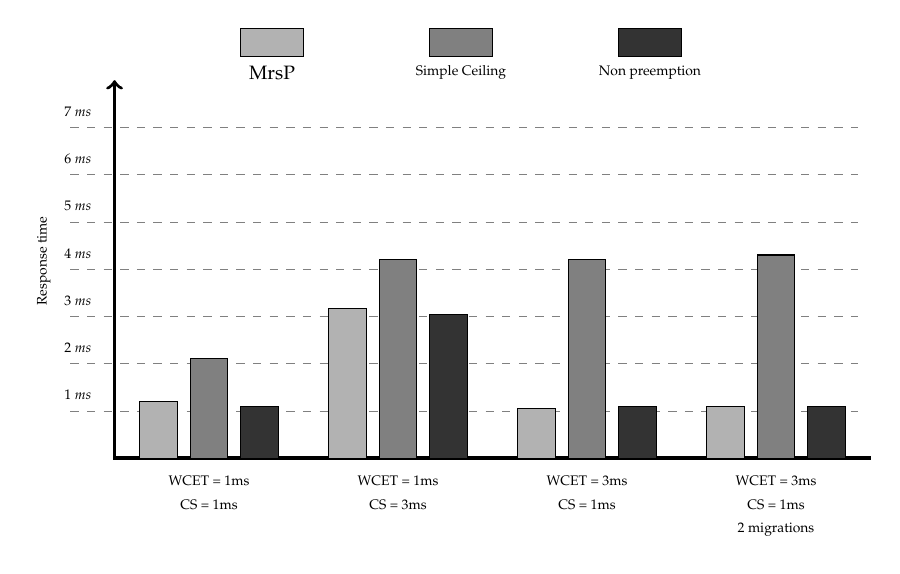
\begin{tikzpicture}[
  xscale=0.8,
  yscale=0.6,
  mrsp/.style={fill=black!30},
  ceiling/.style={ fill=black!50},
  nopreempt/.style={fill=black!80},
  assi/.style={very thick, <-}
  ]
    % Axis
    \coordinate (y) at (0,8);
    \coordinate (x) at (12,0);
    \draw[assi] (y) node[above=-3cm, right=-0.9cm, rotate=90, font=\tiny] {Response time} -- (0,0) -- (x);

    \coordinate (one) at (1.5,-0.5);
    \coordinate (two) at (4.5,-0.5);
    \coordinate (three) at (7.5,-0.5);
    \coordinate (four) at (10.5,-0.5);
%4 gruppi
%3 barre ognuno

\draw[line width=0.1mm, gray, dashed] (-0.7,1)node[black, above=0.2cm, right=-0.2cm] {\tiny 1 $ ms$} -- +(12.5, 0);
\draw[line width=0.1mm, gray, dashed] (-0.7,2)node[black, above=0.2cm, right=-0.2cm] {\tiny 2 $ ms$} -- +(12.5, 0);
\draw[line width=0.1mm, gray, dashed] (-0.7,3)node[black, above=0.2cm, right=-0.2cm] {\tiny 3 $ ms$} -- +(12.5, 0);
\draw[line width=0.1mm, gray, dashed] (-0.7,4)node[black, above=0.2cm, right=-0.2cm] {\tiny 4 $ ms$} -- +(12.5, 0);
\draw[line width=0.1mm, gray, dashed] (-0.7,5)node[black, above=0.2cm, right=-0.2cm] {\tiny 5 $ ms$} -- +(12.5, 0);
\draw[line width=0.1mm, gray, dashed] (-0.7,6)node[black, above=0.2cm, right=-0.2cm] {\tiny 6 $ ms$} -- +(12.5, 0);
\draw[line width=0.1mm, gray, dashed] (-0.7,7)node[black, above=0.2cm, right=-0.2cm] {\tiny 7 $ ms$} -- +(12.5, 0);

\path(one)node[below=+0.1cm]{\tiny CS = 1ms};
\path(one)node[below=-0.2cm]{\tiny WCET = 1ms};

\path(two)node[below=+0.1cm]{\tiny CS = 3ms};
\path(two)node[below=-0.2cm]{\tiny WCET = 1ms};

\path(three)node[below=+0.1cm]{\tiny CS = 1ms};
\path(three)node[below=-0.2cm]{\tiny WCET = 3ms};

\path(four)node[below=+0.1cm]{\tiny CS = 1ms};
\path(four)node[below=-0.2cm]{\tiny WCET = 3ms};
\path(four)node[below=+0.4cm]{\tiny 2 migrations};

%%%%%%%%%%  L1
%  MRSP - CEILING - NP

% PRIMO (1 - 1)
% $L_1$ & \underline{1.206.362} & 2.194.042 & \underline{1.111.517}

% gruppo uno - coord 0 -- 3
\draw[mrsp]  (0.4, 0) rectangle +(0.6, 1.2);
\draw[ceiling]  (1.2, 0) rectangle +(0.6, 2.1);
\draw[nopreempt]  (2, 0) rectangle +(0.6, 1.1);

% SECONDO (SC3 - h1)
%$L_1$ & \underline{3.066.828} & 4.242.092 & \underline{3.177.307}

% gruppo uno - coord 3 -- 6
\draw[mrsp]  (3.4, 0) rectangle +(0.6, 3.17);
\draw[ceiling]  (4.2, 0) rectangle +(0.6, 4.2);
\draw[nopreempt]  (5, 0) rectangle +(0.6, 3.05);

%TERZO (SC1 - H3)
%$L_1$ & \underline{1.053.232} & 4.215.599 & \underline{1.113.397}

% gruppo uno - coord 6 -- 9
\draw[mrsp]  (6.4, 0) rectangle +(0.6, 1.05);
\draw[ceiling]  (7.2, 0) rectangle +(0.6, 4.2);
\draw[nopreempt]  (8, 0) rectangle +(0.6, 1.1);

%QUARTO (SC1 - H3)^2
%$L_1$ & \underline{1.111.410} & 4.312.490 & \underline{1.173.600}

% gruppo uno - coord 9 -- 12
\draw[mrsp]  (9.4, 0) rectangle +(0.6, 1.1);
\draw[ceiling]  (10.2, 0) rectangle +(0.6, 4.3);
\draw[nopreempt]  (11, 0) rectangle +(0.6, 1.1);

%legend
\begin{scope}[shift={(2,8.5)}] 
\draw[mrsp] (0,0) rectangle +(1, 0.6) node[right=-0.4cm, below=0.35cm, color=black]{\scriptsize MrsP};
\draw[ceiling] (3,0) rectangle +(1, 0.6) node[right=-0.4cm, below=0.35cm, color=black]{\tiny Simple Ceiling};
\draw[nopreempt] (6,0) rectangle +(1, 0.6) node[right=-0.4cm, below=0.35cm, color=black]{\tiny Non preemption};
\end{scope}

\end{tikzpicture}}

\newcommand{\confrontoProtocolliHDue}{%
  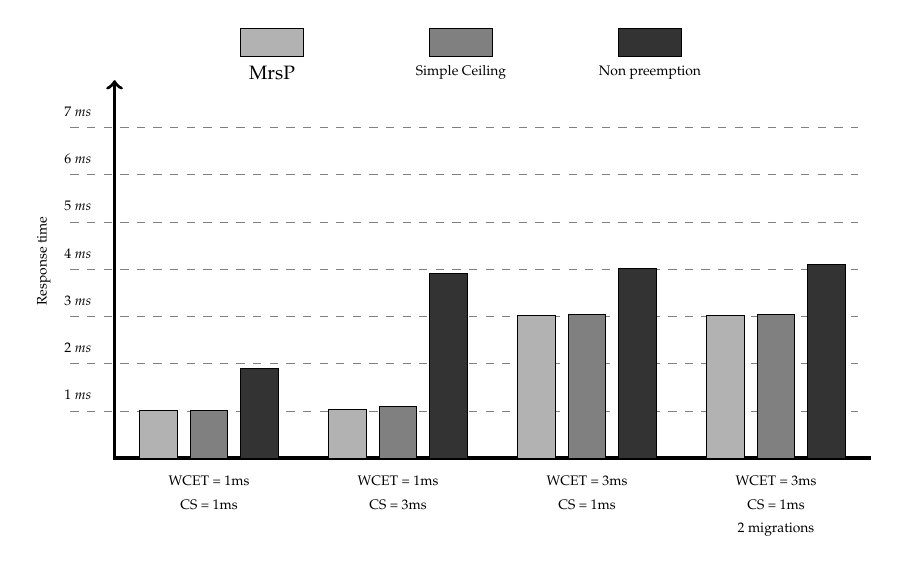
\begin{tikzpicture}[
  xscale=0.8,
  yscale=0.6,
  mrsp/.style={fill=black!30},
  ceiling/.style={ fill=black!50},
  nopreempt/.style={fill=black!80},
  assi/.style={very thick, <-}
  ]
    % Axis
    \coordinate (y) at (0,8);
    \coordinate (x) at (12,0);
    \draw[assi] (y) node[above=-3cm, right=-0.9cm, rotate=90, font=\tiny] {Response time} -- (0,0) -- (x);

    \coordinate (one) at (1.5,-0.5);
    \coordinate (two) at (4.5,-0.5);
    \coordinate (three) at (7.5,-0.5);
    \coordinate (four) at (10.5,-0.5);
%4 gruppi
%3 barre ognuno

\draw[line width=0.1mm, gray, dashed] (-0.7,1)node[black, above=0.2cm, right=-0.2cm] {\tiny 1 $ ms$} -- +(12.5, 0);
\draw[line width=0.1mm, gray, dashed] (-0.7,2)node[black, above=0.2cm, right=-0.2cm] {\tiny 2 $ ms$} -- +(12.5, 0);
\draw[line width=0.1mm, gray, dashed] (-0.7,3)node[black, above=0.2cm, right=-0.2cm] {\tiny 3 $ ms$} -- +(12.5, 0);
\draw[line width=0.1mm, gray, dashed] (-0.7,4)node[black, above=0.2cm, right=-0.2cm] {\tiny 4 $ ms$} -- +(12.5, 0);
\draw[line width=0.1mm, gray, dashed] (-0.7,5)node[black, above=0.2cm, right=-0.2cm] {\tiny 5 $ ms$} -- +(12.5, 0);
\draw[line width=0.1mm, gray, dashed] (-0.7,6)node[black, above=0.2cm, right=-0.2cm] {\tiny 6 $ ms$} -- +(12.5, 0);
\draw[line width=0.1mm, gray, dashed] (-0.7,7)node[black, above=0.2cm, right=-0.2cm] {\tiny 7 $ ms$} -- +(12.5, 0);

\path(one)node[below=+0.1cm]{\tiny CS = 1ms};
\path(one)node[below=-0.2cm]{\tiny WCET = 1ms};

\path(two)node[below=+0.1cm]{\tiny CS = 3ms};
\path(two)node[below=-0.2cm]{\tiny WCET = 1ms};

\path(three)node[below=+0.1cm]{\tiny CS = 1ms};
\path(three)node[below=-0.2cm]{\tiny WCET = 3ms};

\path(four)node[below=+0.1cm]{\tiny CS = 1ms};
\path(four)node[below=-0.2cm]{\tiny WCET = 3ms};
\path(four)node[below=+0.4cm]{\tiny 2 migrations};

%%%%%%%%%%  H2
%  MRSP - CEILING - NP

% PRIMO (1 - 1)
% $H_2$ & 1.098.587 & 1.068.602 & 1.977.039 \\

% gruppo uno - coord 0 -- 3
\draw[mrsp]  (0.4, 0) rectangle +(0.6, 1.005);
\draw[ceiling]  (1.2, 0) rectangle +(0.6, 1.008);
\draw[nopreempt]  (2, 0) rectangle +(0.6, 1.9);

% SECONDO (SC3 - h1)
%$H_2$ & 1.035.721 & 1.141.324 & 3.956.506 \\

% gruppo uno - coord 3 -- 6
\draw[mrsp]  (3.4, 0) rectangle +(0.6, 1.035);
\draw[ceiling]  (4.2, 0) rectangle +(0.6, 1.09);
\draw[nopreempt]  (5, 0) rectangle +(0.6, 3.9);

%TERZO (SC1 - H3)
%$H_2$ & 3.018.344 & 3.071.190 & 4.006.309 \\

% gruppo uno - coord 6 -- 9
\draw[mrsp]  (6.4, 0) rectangle +(0.6, 3.01);
\draw[ceiling]  (7.2, 0) rectangle +(0.6, 3.05);
\draw[nopreempt]  (8, 0) rectangle +(0.6, 4.005);

%QUARTO (SC1 - H3)^2
% $H_2$ & 3.029.214 & 3.131.630 & 4.205.578 \\

% gruppo uno - coord 9 -- 12
\draw[mrsp]  (9.4, 0) rectangle +(0.6, 3.02);
\draw[ceiling]  (10.2, 0) rectangle +(0.6, 3.05);
\draw[nopreempt]  (11, 0) rectangle +(0.6, 4.1);

%legend
\begin{scope}[shift={(2,8.5)}] 
\draw[mrsp] (0,0) rectangle +(1, 0.6) node[right=-0.4cm, below=0.35cm, color=black]{\scriptsize MrsP};
\draw[ceiling] (3,0) rectangle +(1, 0.6) node[right=-0.4cm, below=0.35cm, color=black]{\tiny Simple Ceiling};
\draw[nopreempt] (6,0) rectangle +(1, 0.6) node[right=-0.4cm, below=0.35cm, color=black]{\tiny Non preemption};
\end{scope}

\end{tikzpicture}}

\newcommand{\confrontoProtocolliLTre}{%
  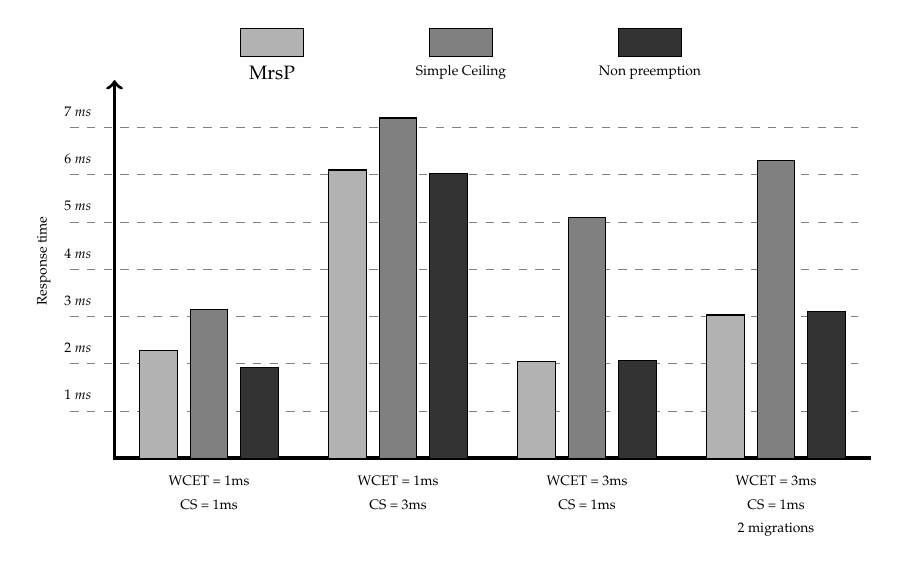
\begin{tikzpicture}[
  xscale=0.8,
  yscale=0.6,
  mrsp/.style={fill=black!30},
  ceiling/.style={ fill=black!50},
  nopreempt/.style={fill=black!80},
  assi/.style={very thick, <-}
  ]
    % Axis
    \coordinate (y) at (0,8);
    \coordinate (x) at (12,0);
    \draw[assi] (y) node[above=-3cm, right=-0.9cm, rotate=90, font=\tiny] {Response time} -- (0,0) -- (x);

    \coordinate (one) at (1.5,-0.5);
    \coordinate (two) at (4.5,-0.5);
    \coordinate (three) at (7.5,-0.5);
    \coordinate (four) at (10.5,-0.5);
%4 gruppi
%3 barre ognuno

\draw[line width=0.1mm, gray, dashed] (-0.7,1)node[black, above=0.2cm, right=-0.2cm] {\tiny 1 $ ms$} -- +(12.5, 0);
\draw[line width=0.1mm, gray, dashed] (-0.7,2)node[black, above=0.2cm, right=-0.2cm] {\tiny 2 $ ms$} -- +(12.5, 0);
\draw[line width=0.1mm, gray, dashed] (-0.7,3)node[black, above=0.2cm, right=-0.2cm] {\tiny 3 $ ms$} -- +(12.5, 0);
\draw[line width=0.1mm, gray, dashed] (-0.7,4)node[black, above=0.2cm, right=-0.2cm] {\tiny 4 $ ms$} -- +(12.5, 0);
\draw[line width=0.1mm, gray, dashed] (-0.7,5)node[black, above=0.2cm, right=-0.2cm] {\tiny 5 $ ms$} -- +(12.5, 0);
\draw[line width=0.1mm, gray, dashed] (-0.7,6)node[black, above=0.2cm, right=-0.2cm] {\tiny 6 $ ms$} -- +(12.5, 0);
\draw[line width=0.1mm, gray, dashed] (-0.7,7)node[black, above=0.2cm, right=-0.2cm] {\tiny 7 $ ms$} -- +(12.5, 0);

\path(one)node[below=+0.1cm]{\tiny CS = 1ms};
\path(one)node[below=-0.2cm]{\tiny WCET = 1ms};

\path(two)node[below=+0.1cm]{\tiny CS = 3ms};
\path(two)node[below=-0.2cm]{\tiny WCET = 1ms};

\path(three)node[below=+0.1cm]{\tiny CS = 1ms};
\path(three)node[below=-0.2cm]{\tiny WCET = 3ms};

\path(four)node[below=+0.1cm]{\tiny CS = 1ms};
\path(four)node[below=-0.2cm]{\tiny WCET = 3ms};
\path(four)node[below=+0.4cm]{\tiny 2 migrations};

%%%%%%%%%%  H2
%  MRSP - CEILING - NP

% PRIMO (1 - 1)
% $L_3$ & 2.351.562 & 3.168.240 & 1.911.890 \\

% gruppo uno - coord 0 -- 3
\draw[mrsp]  (0.4, 0) rectangle +(0.6, 2.28);
\draw[ceiling]  (1.2, 0) rectangle +(0.6, 3.15);
\draw[nopreempt]  (2, 0) rectangle +(0.6, 1.91);

% SECONDO (SC3 - h1)
%$L_3$ & 6.099.752 & 7.209.873 & 6.024.691 \\

% gruppo uno - coord 3 -- 6
\draw[mrsp]  (3.4, 0) rectangle +(0.6, 6.1);
\draw[ceiling]  (4.2, 0) rectangle +(0.6, 7.2);
\draw[nopreempt]  (5, 0) rectangle +(0.6, 6.02);

%TERZO (SC1 - H3)
%$L_3$ & 2.042.122 & 5.169.139 & 2.068.905 \\

% gruppo uno - coord 6 -- 9
\draw[mrsp]  (6.4, 0) rectangle +(0.6, 2.04);
\draw[ceiling]  (7.2, 0) rectangle +(0.6, 5.1);
\draw[nopreempt]  (8, 0) rectangle +(0.6, 2.06);

%QUARTO (SC1 - H3)^2
% $L_5$ & 3.030.634 & 6.309.370 & 3.184.333 \\

% gruppo uno - coord 9 -- 12
\draw[mrsp]  (9.4, 0) rectangle +(0.6, 3.03);
\draw[ceiling]  (10.2, 0) rectangle +(0.6, 6.3);
\draw[nopreempt]  (11, 0) rectangle +(0.6, 3.1);

%legend
\begin{scope}[shift={(2,8.5)}] 
\draw[mrsp] (0,0) rectangle +(1, 0.6) node[right=-0.4cm, below=0.35cm, color=black]{\scriptsize MrsP};
\draw[ceiling] (3,0) rectangle +(1, 0.6) node[right=-0.4cm, below=0.35cm, color=black]{\tiny Simple Ceiling};
\draw[nopreempt] (6,0) rectangle +(1, 0.6) node[right=-0.4cm, below=0.35cm, color=black]{\tiny Non preemption};
\end{scope}

\end{tikzpicture}}
\input{figure/grafico_sched.tex}
% % 50

% SCHED 10132 1646 37787
% RELEASE 5751 1895 23551
% CXS 4233 1283 25619

% % 60

% SCHED 14135 1760 51018
% RELEASE 8980 2036 22429
% CXS 8522 1427 42270


% % 70

% SCHED 12070 1703 48526
% RELEASE 7791 1804 23804
% CXS 6677 1552 37190

% % 75

% SCHED 9362 1454 31108
% RELEASE 6390 1722 22704
% CXS 4931 1323 31229

% % 80

% SCHED 10353 1691 42522
% RELEASE 6634 1867 23694
% CXS 5067 1213 30994

% % 85

% SCHED 8302 1616 29623
% RELEASE 5420 1675 24035
% CXS 3870 1182 27984

% % 90

% SCHED 10132 1646 37787
% RELEASE 5751 1895 23551
% CXS 4233 1283 25619

% % 100

% SCHED 7746 1637 28438
% RELEASE 4366 1870 18062
% CXS 3219 1279 10890
%



\newcommand{\graficoReleaseMIN}{
\begin{tikzpicture}[y=.2cm, x=.7cm,font=\sffamily, yscale=1, xscale=1.5]
  %axis
  \draw (0,0) -- coordinate (x axis mid) (7,0);
      \draw (0,0) -- coordinate (y axis mid) (0,20);
      %ticks
  
  \draw (1,1pt) -- (1,-3pt) node[anchor=north] {\scriptsize 50};
  \draw (2,1pt) -- (2,-3pt) node[anchor=north] {\scriptsize 60};
  \draw (3,1pt) -- (3,-3pt) node[anchor=north] {\scriptsize 70};
  \draw (3.5,1pt) -- (3.5,-5pt) node[anchor=north] {\scriptsize 75};
  \draw (4,1pt) -- (4,-3pt) node[anchor=north] {\scriptsize 80};
  \draw (4.5,1pt) -- (4.5,-5pt) node[anchor=north] {\scriptsize 85};
  \draw (5,1pt) -- (5,-3pt) node[anchor=north] {\scriptsize 90};
  \draw (6,1pt) -- (6,-3pt) node[anchor=north] {\scriptsize 100};

  \foreach \y in {0,5,...,20}
    \draw (1pt,\y) -- (-3pt,\y) 
      node[anchor=east] {\scriptsize \y};

  %labels      
  \node[below=0.8cm] at (x axis mid) {\scriptsize Utilization \%};
  \node[rotate=90, above=0.8cm] at (y axis mid) {\scriptsize Times $10^{-1}$ * $\mu$s};

  %plots
  \draw[color=red, thick] plot[mark=x, mark options={fill=red, xscale=0.75}] 
    file {PFPreleaseMIN.data};

  \draw[color=green, thick] plot[mark=x, mark options={fill=green, xscale=0.75}] 
    file {MRSPreleaseMIN.data};

  %legend
  \begin{scope}[shift={(5,3)}] 
  \draw[color=red, thick] (0,0) -- plot[mark=x, mark options={fill=red, xscale=0.75}] (0.25,0) -- (0.5,0) 
    node[right, color=black]{\scriptsize P-FP};
  \draw[color=green, thick, yshift=0.3cm] (0,0) -- 
    plot[mark=x, mark options={fill=green, xscale=0.75}] (0.25,0) -- (0.5,0)
    node[right, color=black]{\scriptsize P-FP + MrsP};
  \end{scope}

\end{tikzpicture}}

\newcommand{\graficoReleaseMAX}{
\begin{tikzpicture}[y=.2cm, x=.7cm,font=\sffamily, yscale=2, xscale=1.5]
  %axis
  \draw (0,0) -- coordinate (x axis mid) (7,0);
      \draw (0,0) -- coordinate (y axis mid) (0,10);

  \draw (1,1pt) -- (1,-3pt) node[anchor=north] {\scriptsize 50};
  \draw (2,1pt) -- (2,-3pt) node[anchor=north] {\scriptsize 60};
  \draw (3,1pt) -- (3,-3pt) node[anchor=north] {\scriptsize 70};
  \draw (3.5,1pt) -- (3.5,-5pt) node[anchor=north] {\scriptsize 75};
  \draw (4,1pt) -- (4,-3pt) node[anchor=north] {\scriptsize 80};
  \draw (4.5,1pt) -- (4.5,-5pt) node[anchor=north] {\scriptsize 85};
  \draw (5,1pt) -- (5,-3pt) node[anchor=north] {\scriptsize 90};
  \draw (6,1pt) -- (6,-3pt) node[anchor=north] {\scriptsize 100};

  \foreach \y in {0,2,...,10}
    \draw (1pt,\y) -- (-3pt,\y) 
      node[anchor=east] {\scriptsize \y}; 
      
  %labels      
  \node[below=0.8cm] at (x axis mid) {\scriptsize Utilization \%};
  \node[rotate=90, above=0.8cm] at (y axis mid) {\scriptsize Times 10 * $\mu$s};

  %plots
  \draw[color=red, thick] plot[mark=x, mark options={fill=red, yscale=0.5, xscale=0.75}] 
    file {PFPreleaseMAX.data};

  \draw[color=green, thick] plot[mark=x, mark options={fill=green, yscale=0.5, xscale=0.75}] 
    file {MRSPreleaseMAX.data};

    %legend
  \begin{scope}[shift={(5,9)}] 
  \draw[color=red, thick] (0,0) -- plot[mark=x, mark options={fill=red, xscale=0.75}] (0.25,0) -- (0.5,0) 
    node[right, color=black]{\scriptsize P-FP};
  \draw[color=green, thick, yshift=0.15cm] (0,0) -- 
    plot[mark=x, mark options={fill=green, xscale=0.75}] (0.25,0) -- (0.5,0)
    node[right, color=black]{\scriptsize P-FP + MrsP};
  \end{scope}

\end{tikzpicture}}

\newcommand{\graficoReleaseAVG}{
\begin{tikzpicture}[y=.2cm, x=.7cm,font=\sffamily, xscale=1.5]
  %axis

  \draw (0,0) -- coordinate (x axis mid) (7,0);
  \draw (0,0) -- coordinate (y axis mid) (0,20);


  \draw (1,1pt) -- (1,-3pt) node[anchor=north] {\scriptsize 50};
  \draw (2,1pt) -- (2,-3pt) node[anchor=north] {\scriptsize 60};
  \draw (3,1pt) -- (3,-3pt) node[anchor=north] {\scriptsize 70};
  \draw (3.5,1pt) -- (3.5,-5pt) node[anchor=north] {\scriptsize 75};
  \draw (4,1pt) -- (4,-3pt) node[anchor=north] {\scriptsize 80};
  \draw (4.5,1pt) -- (4.5,-5pt) node[anchor=north] {\scriptsize 85};
  \draw (5,1pt) -- (5,-3pt) node[anchor=north] {\scriptsize 90};
  \draw (6,1pt) -- (6,-3pt) node[anchor=north] {\scriptsize 100};

  \foreach \y in {0,5,...,20}
    \draw (1pt,\y) -- (-3pt,\y) 
      node[anchor=east] {\scriptsize \y};
      
  %labels      
  \node[below=0.8cm] at (x axis mid) {\scriptsize Utilization \%};
  \node[rotate=90, above=0.8cm] at (y axis mid) {\scriptsize Times $\mu$s};

  %plots
  \draw[color=red, thick] plot[mark=x, mark options={fill=red, xscale=0.75}] 
    file {PFPreleaseAVG.data};

  \draw[color=green, thick] plot[mark=x, mark options={fill=green, xscale=0.75}] 
    file {MRSPreleaseAVG.data};

  %legend
  \begin{scope}[shift={(5,17)}] 
  \draw[color=red, thick] (0,0) -- plot[mark=x, mark options={fill=red, xscale=0.75}] (0.25,0) -- (0.5,0) 
    node[right, color=black]{\scriptsize P-FP};
  \draw[color=green, thick, yshift=0.3cm] (0,0) -- 
    plot[mark=x, mark options={fill=green, xscale=0.75}] (0.25,0) -- (0.5,0)
    node[right, color=black]{\scriptsize P-FP + MrsP};
  \end{scope}

\end{tikzpicture}}
\input{figure/grafico_cxs.tex}
\newcommand{\RisultatoUnoNoPreempion}{%
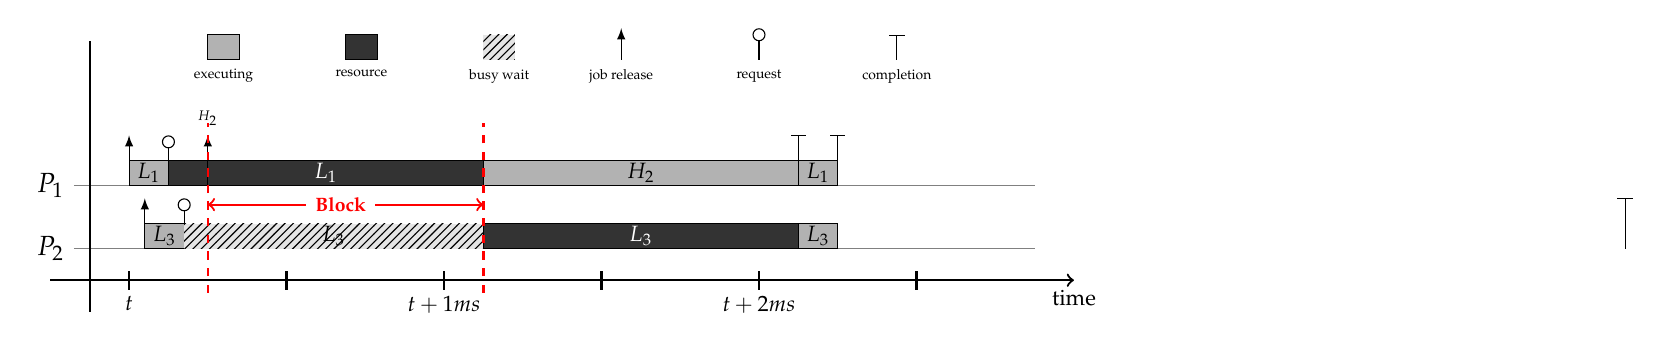
\begin{tikzpicture}[
  yscale = 0.8,
  normal/.style={ fill=black!30},
  resource/.style={ fill=black!80},
  waiting/.style={fill=white},
  busywait/.style={fill=black!10, postaction={pattern=north east lines, very thin}},
  release/.style={-latex},
  request/.style={-o},
  complet/.style={-|},
  every text node part/.style={align=center}
]
%general params
\def\th{.4} %task height
\def\tyDown{0} %task a asse y
\def\tyUp{1}
\def\blockdim{(.4,.4)}
\def\arrowdim{(0,.5)}
\def\arrowdimB{(0,.4)}
\coordinate (legend) at (1,2.5);

%tasklines
\draw[thin, gray] (-.7,\tyDown)node[above,left,black]{$P_2$} -- +(12.2,0);
\draw[thin, gray] (-.7,\tyUp)node[above,left,black]{$P_1$} -- +(12.2,0);

%axes
\draw[thick, black, -] (-.5,-1) -- (-.5, 3.3);
\draw[thick, black, ->] (-1,-.5) -- (12, -.5) node[below] {{\footnotesize time}};

\draw[thick, black, -] (0,-.65) -- (0, -0.35);
\draw[thick, black, -] (2,-.65) -- (2, -0.35);
\draw[thick, black, -] (4,-.65) -- (4, -0.35);
\draw[thick, black, -] (6,-.65) -- (6, -0.35);
\draw[thick, black, -] (8,-.65) -- (8, -0.35);
\draw[thick, black, -] (10,-.65) -- (10, -0.35);

\path(0,-.6)node[below]{{\footnotesize $t$}};
\path(4,-.6)node[below]{{\footnotesize $t + 1 ms$}};
\path(8,-.6)node[below]{{\footnotesize $t + 2 ms$}};

%L1
\draw[release] (0,   \tyUp) -- +(0,0.8);
\draw[normal]  (0,   \tyUp) rectangle +(0.5, \th) node[midway] {{\footnotesize $L_1$}};
\draw[request] (0.5,\tyUp) -- +(0,0.8);
\draw[resource]  (0.5,   \tyUp) rectangle +(4, \th) node[midway,color=white] {{\footnotesize $L_1$}};;

%H2
\draw[release] (1,   \tyUp) -- +(0,0.8) node[above] {{\tiny $H_2$}};
\draw[normal]  (4.5,   \tyUp) rectangle +(4, \th) node[midway] {{\footnotesize $H_2$}};
\draw[complet] (8.5,\tyUp) -- +(0, 0.8);

%L1

\draw[normal]  (8.5,   \tyUp) rectangle +(0.5, \th) node[midway] {{\footnotesize $L_1$}};
\draw[complet] (9,\tyUp) -- +(0, 0.8);

%L3
\draw[release] (0.2,   \tyDown) -- +(0,0.8);
\draw[normal]  (0.2,   \tyDown) rectangle +(0.5, \th) node[midway] {{\footnotesize $L_3$}};
\draw[request] (0.7,\tyDown) -- +(0,0.8);
\fill[busywait] (0.7, \tyDown) rectangle +(3.8, \th) node[midway] {{\footnotesize $L_3$}};

\draw[resource]  (4.5,   \tyDown) rectangle +(4, \th) node[midway,color=white] {{\footnotesize $L_3$}};
\draw[normal]  (8.5,   \tyDown) rectangle +(0.5, \th) node[midway] {{\footnotesize $L_3$}};
\draw[complet] (19,\tyDown) -- +(0, 0.8);


\draw[thick, red, dashed, -] (1,-0.7) -- (1, 2);
\draw[thick, red, <->] (1,.70) -- (4.5, .70) node[midway, fill=white, xshift=-1.75] {{\scriptsize \textbf{Block}}};
\draw[thick, red, dashed, -] (4.5,-0.7) -- (4.5, 2);

\draw[normal]   ($(   0,0.5) + (legend)$) node[below, xshift=0.2cm]{\tiny executing} rectangle +\blockdim;
\draw[resource] ($(1.75,0.5) + (legend)$) node[below, xshift=0.2cm]{\tiny resource} rectangle +\blockdim;
\fill[busywait] ($( 3.5,0.5) + (legend)$) node[below, xshift=0.2cm]{\tiny busy wait} rectangle +\blockdim;
\draw[release]  ($(5.25,0.5) + (legend)$) node[below]{\tiny job release}      -- +\arrowdim;
\draw[request]  ($(   7,0.5) + (legend)$) node[below]{\tiny request}     -- +\arrowdim;
\draw[complet]  ($(8.75,0.5) + (legend)$) node[below]{\tiny completion}   -- +\arrowdimB;

\end{tikzpicture}
}

\newcommand{\RisultatoUnoCeiling}{%
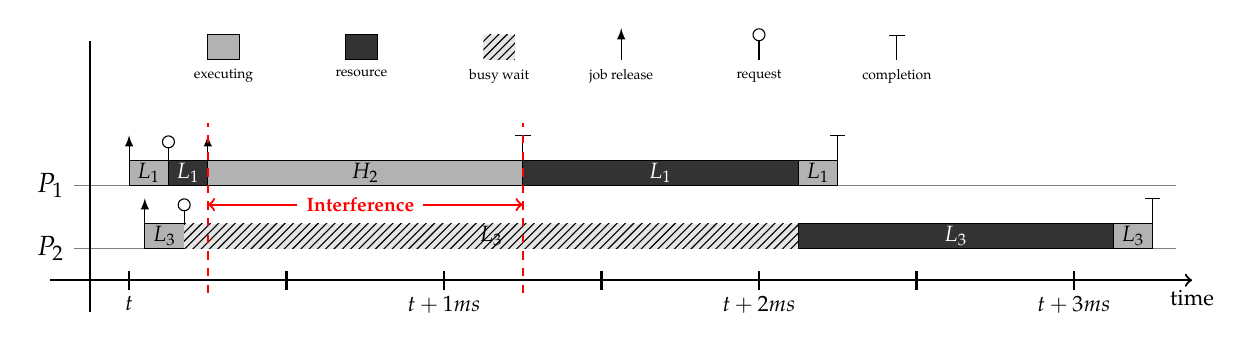
\begin{tikzpicture}[
  yscale = 0.8,
  normal/.style={ fill=black!30},
  resource/.style={ fill=black!80},
  waiting/.style={fill=white},
  busywait/.style={fill=black!10, postaction={pattern=north east lines, very thin}},
  release/.style={-latex},
  request/.style={-o},
  complet/.style={-|},
  every text node part/.style={align=center}
]
%general params
\def\th{.4} %task height
\def\tyDown{0} %task a asse y
\def\tyUp{1}
\def\blockdim{(.4,.4)}
\def\arrowdim{(0,.5)}
\def\arrowdimB{(0,.4)}
\coordinate (legend) at (1,2.5);

%tasklines
\draw[thin, gray] (-.7,\tyDown)node[above,left,black]{$P_2$} -- +(14,0);
\draw[thin, gray] (-.7,\tyUp)node[above,left,black]{$P_1$} -- +(14,0);

%axes
\draw[thick, black, -] (-.5,-1) -- (-.5, 3.3);
\draw[thick, black, ->] (-1,-.5) -- (13.5, -.5) node[below] {{\footnotesize time}};

\draw[thick, black, -] (0,-.65) -- (0, -0.35);
\draw[thick, black, -] (2,-.65) -- (2, -0.35);
\draw[thick, black, -] (4,-.65) -- (4, -0.35);
\draw[thick, black, -] (6,-.65) -- (6, -0.35);
\draw[thick, black, -] (8,-.65) -- (8, -0.35);
\draw[thick, black, -] (10,-.65) -- (10, -0.35);
\draw[thick, black, -] (12,-.65) -- (12, -0.35);

\path(0,-.6)node[below]{{\footnotesize $t$}};
\path(4,-.6)node[below]{{\footnotesize $t + 1 ms$}};
\path(8,-.6)node[below]{{\footnotesize $t + 2 ms$}};
\path(12,-.6)node[below]{{\footnotesize $t + 3 ms$}};


%L1
\draw[release] (0,   \tyUp) -- +(0,0.8);
\draw[normal]  (0,   \tyUp) rectangle +(0.5, \th) node[midway] {{\footnotesize $L_1$}};
\draw[request] (0.5,\tyUp) -- +(0,0.8);
\draw[resource]  (0.5,   \tyUp) rectangle +(0.5, \th) node[midway,color=white] {{\footnotesize $L_1$}};;

%H2
\draw[release] (1,   \tyUp) -- +(0,0.8);
\draw[normal]  (1,   \tyUp) rectangle +(4, \th) node[midway] {{\footnotesize $H_2$}};
\draw[complet] (5,\tyUp) -- +(0, 0.8);

%L1

\draw[resource]  (5,   \tyUp) rectangle +(3.5, \th) node[midway,color=white] {{\footnotesize $L_1$}};;
\draw[normal]  (8.5,   \tyUp) rectangle +(0.5, \th) node[midway] {{\footnotesize $L_1$}};
\draw[complet] (9,\tyUp) -- +(0, 0.8);

%L3
\draw[release] (0.2,   \tyDown) -- +(0,0.8);
\draw[normal]  (0.2,   \tyDown) rectangle +(0.5, \th) node[midway] {{\footnotesize $L_3$}};
\draw[request] (0.7,\tyDown) -- +(0,0.8);
\fill[busywait] (0.7, \tyDown) rectangle +(7.8, \th) node[midway] {{\footnotesize $L_3$}};

\draw[resource]  (8.5,   \tyDown) rectangle +(4, \th) node[midway,color=white] {{\footnotesize $L_3$}};
\draw[normal]  (12.5,   \tyDown) rectangle +(0.5, \th) node[midway] {{\footnotesize $L_3$}};
\draw[complet] (13,\tyDown) -- +(0, 0.8);


\draw[thick, red, dashed, -] (1,-0.7) -- (1, 2);
\draw[thick, red, <->] (1,.70) -- (5, .70) node[midway, fill=white, xshift=-1.75] {{\scriptsize \textbf{Interference}}};
\draw[thick, red, dashed, -] (5,-0.7) -- (5, 2);

\draw[normal]   ($(   0,0.5) + (legend)$) node[below, xshift=0.2cm]{\tiny executing} rectangle +\blockdim;
\draw[resource] ($(1.75,0.5) + (legend)$) node[below, xshift=0.2cm]{\tiny resource} rectangle +\blockdim;
\fill[busywait] ($( 3.5,0.5) + (legend)$) node[below, xshift=0.2cm]{\tiny busy wait} rectangle +\blockdim;
\draw[release]  ($(5.25,0.5) + (legend)$) node[below]{\tiny job release}      -- +\arrowdim;
\draw[request]  ($(   7,0.5) + (legend)$) node[below]{\tiny request}     -- +\arrowdim;
\draw[complet]  ($(8.75,0.5) + (legend)$) node[below]{\tiny completion}   -- +\arrowdimB;

\end{tikzpicture}
}

\newcommand{\RisultatoUnoMrsP}{%
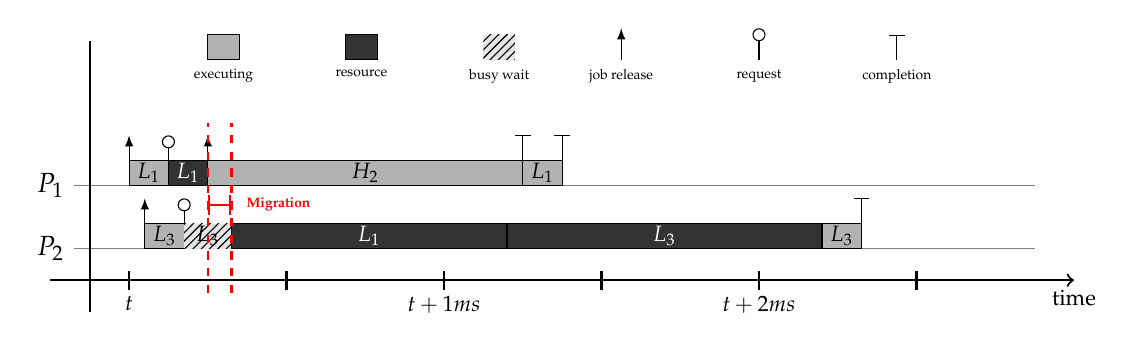
\begin{tikzpicture}[
  yscale = 0.8,
  normal/.style={ fill=black!30},
  resource/.style={ fill=black!80},
  waiting/.style={fill=white},
  busywait/.style={fill=black!10, postaction={pattern=north east lines, very thin}},
  release/.style={-latex},
  request/.style={-o},
  complet/.style={-|},
  every text node part/.style={align=center}
]
%general params
\def\th{.4} %task height
\def\tyDown{0} %task a asse y
\def\tyUp{1}
\def\blockdim{(.4,.4)}
\def\arrowdim{(0,.5)}
\def\arrowdimB{(0,.4)}
\coordinate (legend) at (1,2.5);

%tasklines
\draw[thin, gray] (-.7,\tyDown)node[above,left,black]{$P_2$} -- +(12.2,0);
\draw[thin, gray] (-.7,\tyUp)node[above,left,black]{$P_1$} -- +(12.2,0);

%axes
\draw[thick, black, -] (-.5,-1) -- (-.5, 3.3);
\draw[thick, black, ->] (-1,-.5) -- (12, -.5) node[below] {{\footnotesize time}};

\draw[thick, black, -] (0,-.65) -- (0, -0.35);
\draw[thick, black, -] (2,-.65) -- (2, -0.35);
\draw[thick, black, -] (4,-.65) -- (4, -0.35);
\draw[thick, black, -] (6,-.65) -- (6, -0.35);
\draw[thick, black, -] (8,-.65) -- (8, -0.35);
\draw[thick, black, -] (10,-.65) -- (10, -0.35);

\path(0,-.6)node[below]{{\footnotesize $t$}};
\path(4,-.6)node[below]{{\footnotesize $t + 1 ms$}};
\path(8,-.6)node[below]{{\footnotesize $t + 2 ms$}};

%L1
\draw[release] (0,   \tyUp) -- +(0,0.8);
\draw[normal]  (0,   \tyUp) rectangle +(0.5, \th) node[midway] {{\footnotesize $L_1$}};
\draw[request] (0.5,\tyUp) -- +(0,0.8);
\draw[resource]  (0.5,   \tyUp) rectangle +(0.5, \th) node[midway,color=white] {{\footnotesize $L_1$}};;

%H2
\draw[release] (1,   \tyUp) -- +(0,0.8);
\draw[normal]  (1,   \tyUp) rectangle +(4, \th) node[midway] {{\footnotesize $H_2$}};
\draw[complet] (5,\tyUp) -- +(0, 0.8);

%L3
\draw[release] (0.2,   \tyDown) -- +(0,0.8);
\draw[normal]  (0.2,   \tyDown) rectangle +(0.5, \th) node[midway] {{\footnotesize $L_3$}};
\draw[request] (0.7,\tyDown) -- +(0,0.8);
\fill[busywait] (0.7, \tyDown) rectangle +(0.6, \th) node[midway] {{\footnotesize $L_3$}};

%L1

\draw[resource]  (1.3,   \tyDown) rectangle +(3.5, \th) node[midway,color=white] {{\footnotesize $L_1$}};;

%L3

\draw[resource]  (4.8,   \tyDown) rectangle +(4, \th) node[midway,color=white] {{\footnotesize $L_3$}};
\draw[normal]  (8.8,   \tyDown) rectangle +(0.5, \th) node[midway] {{\footnotesize $L_3$}};
\draw[complet] (9.3,\tyDown) -- +(0, 0.8);

% L1

\draw[normal]  (5,   \tyUp) rectangle +(0.5, \th) node[midway] {{\footnotesize $L_1$}};
\draw[complet] (5.5,\tyUp) -- +(0, 0.8);

\draw[thick, red, dashed, -] (1,-0.7) -- (1, 2);
\draw[thick, red, |-|] (1,.70) -- (1.3, .70) node[right, fill=white, xshift=1.75] {{\tiny \textbf{Migration}}};
\draw[thick, red, dashed, -] (1.3,-0.7) -- (1.3, 2);

\draw[normal]   ($(   0,0.5) + (legend)$) node[below, xshift=0.2cm]{\tiny executing} rectangle +\blockdim;
\draw[resource] ($(1.75,0.5) + (legend)$) node[below, xshift=0.2cm]{\tiny resource} rectangle +\blockdim;
\fill[busywait] ($( 3.5,0.5) + (legend)$) node[below, xshift=0.2cm]{\tiny busy wait} rectangle +\blockdim;
\draw[release]  ($(5.25,0.5) + (legend)$) node[below]{\tiny job release}      -- +\arrowdim;
\draw[request]  ($(   7,0.5) + (legend)$) node[below]{\tiny request}     -- +\arrowdim;
\draw[complet]  ($(8.75,0.5) + (legend)$) node[below]{\tiny completion}   -- +\arrowdimB;

\end{tikzpicture}
}
\newcommand{\smallqueueoverhead}[2]{%

\draw[queuesty] (#1)node[right,xshift=.4cm,yshift=.-0.4cm]{\sffamily #2}-- ++(.2,.15)-- ++(1.15,0)-- ++(0,-.3)-- ++(-1.2,0)-- cycle;

\draw[fill=blue!90] (#1) ++ (.3,.15)rectangle +(.3,-.3);
\draw[fill=blue!70,postaction={pattern=north east lines, very thin, pattern color=white}] (#1) ++ (.65,.15)rectangle +(.3,-.3);
\draw[fill=blue!70,postaction={pattern=north east lines, very thin, pattern color=white}] (#1) ++ (1,.15)rectangle +(.3,-.3);}

\newcommand{\bigqueueoverhead}[2]{%
\draw[queuesty] (#1)node[right,xshift=.2cm]{\sffamily #2}-- ++(.3,.3)-- ++(.8,0)-- ++(0,-.6)-- ++(-.8,0)-- cycle;}

\newcommand{\overheadsSuffered}[2]{%
\begin{tikzpicture}[
  xscale=#1,
  yscale=#2,
  every node/.append style={transform shape},
  queuesty/.style={fill=white, very thick, font=\tiny},
  srpsty/.style={fill=white, draw, circle, text width=.17cm, font=\tiny, very thick},
  numsty/.style={text width=.1cm, font=\tiny},
  arrow/.style={->},
  littletext/.style={font=\sffamily\tiny,inner sep=0pt,outer sep=-2pt,fill=white},
  ressty/.style={fill=red!30, draw, very thick, rounded corners=5pt},
  emptytask/.style={rectangle, minimum width=.7cm,font=\footnotesize},
  taskHolder/.style={fill=blue!90, draw, rectangle, minimum width=.7cm,font=\footnotesize},
  taskWaiting/.style={fill=blue!70, draw, rectangle, minimum width=.7cm,font=\footnotesize,postaction={pattern=north east lines, very thin, pattern color=white}},
  taskAccess/.style={fill=blue!30, draw, rectangle, minimum width=.7cm,font=\footnotesize},
  taskNotAccess/.style={fill=white, draw, rectangle, minimum width=.7cm,font=\footnotesize}]

\def\blockdim{(.7,.25)}

\draw[arrow] (2.2,5.25) to[out=90,in=0] (2.35,6.6);

\begin{scope}[xshift=2.2cm, yshift=5cm]
  \coordinate (SRPnode) at (0,0);

  \draw[dashed,purple] (-1.5,-0.78) -- (0.27,-0.78);

  \node[taskNotAccess]  (T1)  at (-0.8,-0.50)  {};
  \node[emptytask]      (TP1) at (-0.8,-0.75) {$\cdots$};
  \node[taskWaiting]     (T2)  at (-0.8,-1.00)  {};
  \node[emptytask]      (TP1) at (-0.8,-1.25) {$\cdots$};
  \node[taskAccess]     (T3)  at (-0.8,-1.50)  {};
  \node[emptytask]      (TP1) at (-0.8,-1.75) {$\cdots$};
  \node[taskNotAccess]  (T4)  at (-0.8,-2.00)  {};
  \node[emptytask]      (TP1) at (-0.8,-2.25) {$\cdots$};
  \node[taskNotAccess]     (T5)  at (-0.8,-2.50)  {};

  \draw[dashed, thin] ([shift={(-1.5,0)}]SRPnode) node[right,xshift=.1cm,littletext]{Partition$_2$} rectangle ([shift={(.3,-.15)}]T5.south-|SRPnode.east);

  \node[srpsty] (SRP) at (SRPnode) {}; \node[font=\sffamily\tiny] at(SRPnode.west){SRP};
  \draw[arrow] (T2.east) to[out=0,in=270] (SRP.south);

  \draw[red] ([shift={(-.4,.17)}]T2) rectangle ([shift={(.25,-.05)}]T5.south-|T5.east);

  \draw[arrow,red] (-0.35,-3.05) -- ([shift={(.1,-.05)}]T5.south-|T3.east);

\end{scope}

% SMUSSARE UN POCHETTO LA TRAIETTORIA??
\draw[arrow] (1.8,5.80) to[out=10,in=0] (2.35,6.55);
\draw (0,5.20) to[out=90,in=190] (1.8,5.80);

\begin{scope}[yshift=5cm]
  \coordinate (SRPnode) at (0,0);

  \draw[dashed,purple] (-1.5,-0.78) -- (0.27,-0.78);

  \node[taskNotAccess]  (T1)  at (-0.8,-0.50)  {};
  \node[emptytask]      (TP1) at (-0.8,-0.75) {$\cdots$};
  \node[taskAccess]     (T2)  at (-0.8,-1.00)  {};
  \node[emptytask]      (TP1) at (-0.8,-1.25) {$\cdots$};
  \node[taskHolder]     (T3)  at (-0.8,-1.50)  {};
  \node[emptytask]      (TP1) at (-0.8,-1.75) {$\cdots$};
  \node[taskNotAccess]  (T4)  at (-0.8,-2.00)  {};
  \node[emptytask]      (TP1) at (-0.8,-2.25) {$\cdots$};
  \node[taskAccess]     (T5)  at (-0.8,-2.50)  {};

  \draw[dashed, thin] ([shift={(-1.5,0)}]SRPnode) node[right,xshift=.1cm,littletext]{Partition$_1$} rectangle ([shift={(.3,-.15)}]T5.south-|SRPnode.east);

  \node[srpsty] (SRP) at (SRPnode) {}; \node[font=\sffamily\tiny] at(SRPnode.west){SRP};
  \draw[arrow] (T3.east) to[out=0,in=270] (SRP.south);

   \draw[red] ([shift={(-.4,.17)}]T2) rectangle ([shift={(.25,-.05)}]T5.south-|T3.east) node[right,fill=none,red,littletext, yshift=.2cm]{(ii)};

  \draw[red] ([shift={(-.6,.2)}]T3) node[right,fill=none,red,littletext]{(i)} rectangle ([shift={(.05,-.05)}]T3.south-|T3.east);

  \draw[arrow,red] (-0.35,-3.2) -- ([shift={(.1,-.05)}]T5.south-|T3.east);

  \draw[red]  (-0.35,-3.2) node[right,fill=white,red,littletext,xshift=2.1cm]{(iii)} -- (4.05,-3.2);

\end{scope}

\draw[arrow] (4.4,5.25) to[out=90,in=0] (2.35,6.65);

\begin{scope}[xshift=4.4cm, yshift=5cm]
  \coordinate (SRPnode) at (0,0);

  \draw[dashed, purple] (-1.5,-1.28) -- (0.27,-1.28);

  \node[taskNotAccess]  (T1)  at (-0.8,-0.50)  {};
  \node[emptytask]      (TP1) at (-0.8,-0.75) {$\cdots$};
  \node[taskNotAccess]  (T2)  at (-0.8,-1.00)  {};
  \node[emptytask]      (TP1) at (-0.8,-1.25) {$\cdots$};
  \node[taskAccess]     (T3)  at (-0.8,-1.50)  {};
  \node[emptytask]      (TP1) at (-0.8,-1.75) {$\cdots$};
  \node[taskWaiting]    (T4)  at (-0.8,-2.00)  {};
  \node[emptytask]      (TP1) at (-0.8,-2.25) {$\cdots$};
  \node[taskAccess]     (T5)  at (-0.8,-2.50)  {};

  \draw[dashed, thin] ([shift={(-1.5,0)}]SRPnode) node[right,xshift=.1cm,littletext]{Partition$_3$} rectangle ([shift={(.3,-.15)}]T5.south-|SRPnode.east);

  \node[srpsty] (SRP) at (SRPnode) {}; \node[font=\sffamily\tiny] at(SRPnode.west){SRP};
  \draw[arrow] (T4.east) to[out=0,in=270] (SRP.south);

  \draw[red] ([shift={(-.4,.17)}]T3) rectangle ([shift={(.25,-.05)}]T5.south-|T5.east);

  \draw[arrow,red] (-0.35,-3.2) -- ([shift={(.1,-.05)}]T5.south-|T3.east);

\end{scope}

\begin{scope}[xshift=6.6cm, yshift=5cm]
  \coordinate (SRPnode) at (0,0);

  \node[taskNotAccess]  (T1)  at (-0.8,-0.50)  {};
  \node[emptytask]      (TP1) at (-0.8,-0.75) {$\cdots$};
  \node[taskNotAccess]  (T2)  at (-0.8,-1.00)  {};
  \node[emptytask]      (TP1) at (-0.8,-1.25) {$\cdots$};
  \node[taskNotAccess]  (T3)  at (-0.8,-1.50)  {};
  \node[emptytask]      (TP1) at (-0.8,-1.75) {$\cdots$};
  \node[taskNotAccess]  (T4)  at (-0.8,-2.00)  {};
  \node[emptytask]      (TP1) at (-0.8,-2.25) {$\cdots$};
  \node[taskNotAccess]  (T5)  at (-0.8,-2.50)  {};

  \draw[dashed, thin] ([shift={(-1.5,0)}]SRPnode) node[right,xshift=.1cm,littletext]{Partition$_4$} rectangle ([shift={(.3,-.15)}]T5.south-|SRPnode.east);

  \node[srpsty] (SRP) at (SRPnode) {}; \node[font=\sffamily\tiny] at(SRPnode.west){SRP};
\end{scope}

\begin{scope}[yshift=7cm]
\draw[ressty] (-0.5,-.65) rectangle +(1.5,.5) node[midway, font=\tiny]{resource};
\smallqueueoverhead{1.0,-0.4}{FIFO}
\draw[|-|] (1.2, -.02) -- ++(1.15,0)node[midway,fill=white,font=\tiny]{$3$};
\end{scope}

\begin{scope}[yshift=7.5cm]
  \draw[taskNotAccess]   (-1.5,0) node[right, xshift=0.8cm, yshift=.125cm]{\tiny Doesn't need resource} rectangle +\blockdim;
  \draw[taskAccess]   (-1.5,0.5) node[right, xshift=0.8cm, yshift=.125cm]{\tiny Needs resource access} rectangle +\blockdim;
  \draw[taskHolder]   (2,0.5) node[right, xshift=0.8cm, yshift=.125cm]{\tiny Lock Holder} rectangle +\blockdim;
  \draw[taskWaiting]   (2,0) node[right, xshift=0.8cm, yshift=.125cm]{\tiny Queued and waiting} rectangle +\blockdim;

  \draw[dashed,purple] (4.5,0.6) node[right, xshift=0.7cm, black]{\tiny Local ceiling} -- +(0.7,0);
\end{scope}

\end{tikzpicture}}

\newcommand{\dataCPU}[1]{
  \node[below] (F1)  at (-0.8,-0.50)  {\tiny (task*) scheduled};
  \node[below, xshift=-0.2cm] (F2)  at (-0.8,-1.00)  {\tiny (int) cpu};
  \node[below, xshift=0.05cm] (F3)  at (-0.8,-1.50)  {\tiny (queue*) ready\_queue};
  \node[below, xshift=-0.08cm] (F4)  at (-0.8,-2.00)  {\tiny (int) ceiling};
  \node[below, xshift=-0.45cm] (F5)  at (-0.8,-2.50)  {\tiny (spinlock) {red lock}};
  \node[below, xshift=-0.3cm] (F6)  at (-0.8,-3)  {\tiny (sem*) mrsp};

  \draw[dashed, thin] ([shift={(-0.1,+0.1)}]F1.north-|F5.west) node[right,xshift=.3cm,littletext]{Partition$_#1$} rectangle ([shift={(0.1,-0.1)}]F6.south-|F3.east);
  }

\newcommand{\dataMRSP}{
  \node[below] (F1)  at (-0.8,-0.50)  {\tiny (task*) lock holder};
  \node[below, xshift=-0.1cm] (F2)  at (-0.8,-1.00)  {\tiny (int*) ceilings};
  \node[below, xshift=-0.4cm] (F3)  at (-0.8,-1.50)  {\tiny (queue*) tasks};
  \node[below, xshift=-0.5cm] (F4)  at (-0.8,-2.00)  {\tiny (spinlock) {red lock}};

  \draw[dashed, thin] ([shift={(-0.1,+0.1)}]F1.north-|F4.west) node[right,xshift=.3cm,littletext]{MrsP} rectangle ([shift={(0.1,-0.1)}]F4.south-|F1.east);
}

\newcommand{\data}[2]{
\begin{tikzpicture}[
  xscale=#1,
  yscale=#2,
  every node/.append style={transform shape},
  queuesty/.style={fill=white, very thick, font=\tiny},
  srpsty/.style={fill=white, draw, circle, text width=.17cm, font=\tiny, very thick},
  numsty/.style={text width=.1cm, font=\tiny},
  arrow/.style={->},
  littletext/.style={font=\sffamily\tiny,inner sep=0pt,outer sep=-2pt,fill=white},
  ressty/.style={fill=red!30, draw, very thick, rounded corners=5pt},
  empty/.style={rectangle, minimum width=.7cm,font=\footnotesize}]

\begin{scope}
  \node[empty]      (C1) at (-0.8,-3.9) {$\cdots$};
  \dataCPU{i}
  \node[empty]      (C2) at (-0.8,0) {$\cdots$};
\end{scope}

\begin{scope} [xshift=5cm, yshift=-0.2cm]
  \dataMRSP
\end{scope}

\draw[arrow] (0,-3.25) to[out=0,in=180] (2.5,-2.5);

\end{tikzpicture}}

\tikzset{
%Define standard arrow tip
>=stealth',
%Define style for different line styles
help lines/.style={dashed, thick},
axis/.style={very thick, <->},
important line/.style={thick},
connection/.style={thick, dotted},
}

\newcommand{\overheadsLock}{%
  \begin{tikzpicture}[
  fun/.style={ fill=black!30},
  migr/.style={ fill=black!80}
  ]
    % Axis
    \coordinate (y) at (0,9);
    \coordinate (x) at (6,0);
    \draw[axis] (y) node[above=-6cm, right=-0.9cm, rotate=90, font=\small] {Times $\mu$s} -- (0,0) --  (x);

\draw[line width=0.1mm, gray, dashed] (-0.35,1)node[black, above=0.2cm, right=-0.2cm] {\tiny 1 } -- +(6, 0);
\draw[line width=0.1mm, gray, dashed] (-0.35,2)node[black, above=0.2cm, right=-0.2cm] {\tiny 2 } -- +(6, 0);
\draw[line width=0.1mm, gray, dashed] (-0.35,3)node[black, above=0.2cm, right=-0.2cm] {\tiny 3 } -- +(6, 0);
\draw[line width=0.1mm, gray, dashed] (-0.35,4)node[black, above=0.2cm, right=-0.2cm] {\tiny 4 } -- +(6, 0);
\draw[line width=0.1mm, gray, dashed] (-0.35,5)node[black, above=0.2cm, right=-0.2cm] {\tiny 5 } -- +(6, 0);
\draw[line width=0.1mm, gray, dashed] (-0.35,6)node[black, above=0.2cm, right=-0.2cm] {\tiny 6 } -- +(6, 0);
\draw[line width=0.1mm, gray, dashed] (-0.35,7)node[black, above=0.2cm, right=-0.2cm] {\tiny 7 } -- +(6, 0);
\draw[line width=0.1mm, gray, dashed] (-0.35,8)node[black, above=0.2cm, right=-0.2cm] {\tiny 8 } -- +(6, 0);

\draw[fun]  (1, 8.5) rectangle +(0.5, 0.3);
\path(1.3, 8.9)node[above] {{\small Function}};
\draw[migr]  (3, 8.5) rectangle +(0.5, 0.3);
\path(3.3, 8.8)node[above] {{\small Migration}};

\path(1.5,0)node[below, xshift=-0.2cm]{\small PCP/SRP};
\path(3,0)node[below]{\small yield $P_i$};
\path(4.5,0)node[below]{\small busy};
\path(4.5,0)node[below, yshift=-0.3cm]{\small wait};

\draw[fun]  (1.2, 0) rectangle +(0.6, 0.8);

\draw[fun]  (2.7, 0) rectangle +(0.6, 2);
\draw[migr]  (2.7, 2) rectangle +(0.6, 6);

\draw[fun]  (4.2, 0) rectangle +(0.6, 0.5);

\end{tikzpicture}}

\newcommand{\overheadsRelease}{%
  \begin{tikzpicture}[
  fun/.style={ fill=black!30},
  migr/.style={ fill=black!80}
  ]
    % Axis
    \coordinate (y) at (0,9);
    \coordinate (x) at (4,0);
    \draw[axis] (y) node[above=-6cm, right=-0.9cm, rotate=90, font=\small] {Times $\mu$s} -- (0,0) --  (x);

\draw[line width=0.1mm, gray, dashed] (-0.35,1)node[black, above=0.2cm, right=-0.2cm] {\tiny 1 } -- +(4, 0);
\draw[line width=0.1mm, gray, dashed] (-0.35,2)node[black, above=0.2cm, right=-0.2cm] {\tiny 2 } -- +(4, 0);
\draw[line width=0.1mm, gray, dashed] (-0.35,3)node[black, above=0.2cm, right=-0.2cm] {\tiny 3 } -- +(4, 0);
\draw[line width=0.1mm, gray, dashed] (-0.35,4)node[black, above=0.2cm, right=-0.2cm] {\tiny 4 } -- +(4, 0);
\draw[line width=0.1mm, gray, dashed] (-0.35,5)node[black, above=0.2cm, right=-0.2cm] {\tiny 5 } -- +(4, 0);
\draw[line width=0.1mm, gray, dashed] (-0.35,6)node[black, above=0.2cm, right=-0.2cm] {\tiny 6 } -- +(4, 0);
\draw[line width=0.1mm, gray, dashed] (-0.35,7)node[black, above=0.2cm, right=-0.2cm] {\tiny 7 } -- +(4, 0);
\draw[line width=0.1mm, gray, dashed] (-0.35,8)node[black, above=0.2cm, right=-0.2cm] {\tiny 8 } -- +(4, 0);

\draw[fun]  (1, 8.5) rectangle +(0.5, 0.3);
\path(1.3, 8.9)node[above] {{\small Function}};
\draw[migr]  (3, 8.5) rectangle +(0.5, 0.3);
\path(3.3, 8.8)node[above] {{\small Migration}};

\path(1.5,0)node[below, xshift=-0.3cm]{\small PCP/SRP};
\path(3,0)node[below, xshift=0.3cm]{\small migrate next};
\path(3,0)node[below, yshift=-0.3cm, xshift=0.3cm]{\small lock holder};

\draw[fun]  (1.2, 0) rectangle +(0.6, 0.8);

\draw[fun]  (2.7, 0) rectangle +(0.6, 2);
\draw[migr]  (2.7, 2) rectangle +(0.6, 6);

\end{tikzpicture}}

\newcommand{\overheadsFS}{%
  \begin{tikzpicture}[
  fun/.style={ fill=black!30},
  migr/.style={ fill=black!80}
  ]
    % Axis
    \coordinate (y) at (0,9);
    \coordinate (x) at (6,0);
    \draw[axis] (y) node[above=-6cm, right=-0.9cm, rotate=90, font=\small] {Times $10 * \mu$s} -- (0,0) --  (x);

\draw[line width=0.1mm, gray, dashed] (-0.35,1)node[black, above=0.2cm, right=-0.2cm] {\tiny 1 } -- +(6, 0);
\draw[line width=0.1mm, gray, dashed] (-0.35,2)node[black, above=0.2cm, right=-0.2cm] {\tiny 2 } -- +(6, 0);
\draw[line width=0.1mm, gray, dashed] (-0.35,3)node[black, above=0.2cm, right=-0.2cm] {\tiny 3 } -- +(6, 0);
\draw[line width=0.1mm, gray, dashed] (-0.35,4)node[black, above=0.2cm, right=-0.2cm] {\tiny 4 } -- +(6, 0);
\draw[line width=0.1mm, gray, dashed] (-0.35,5)node[black, above=0.2cm, right=-0.2cm] {\tiny 5 } -- +(6, 0);
\draw[line width=0.1mm, gray, dashed] (-0.35,6)node[black, above=0.2cm, right=-0.2cm] {\tiny 6 } -- +(6, 0);

\draw[fun]  (1, 8.5) rectangle +(0.5, 0.3);
\path(1.3, 8.9)node[above] {{\small Function}};
\draw[migr]  (3, 8.5) rectangle +(0.5, 0.3);
\path(3.3, 8.8)node[above] {{\small Migration}};

\path(1.5,0)node[below, xshift=-0.2cm]{\small preempted};
\path(3,0)node[below]{\small processor};
\path(3,0)node[below,yshift=-0.3cm]{\small available};
\path(4.5,0)node[below, xshift=0.2cm]{\small default};
\path(4.5,0)node[below,yshift=-0.3cm, xshift=0.2cm]{\small migration};

\draw[fun]  (1.2, 0) rectangle +(0.6, 2.4);
\draw[migr]  (1.2, 2.4) rectangle +(0.6, 3.7);

\draw[fun]  (2.7, 0) rectangle +(0.6, 0.3);
\draw[migr]  (2.7, 0.3) rectangle +(0.6, 0.6);

\draw[fun]  (4.2, 0) rectangle +(0.6, 0.2);
\draw[migr]  (4.2, 0.2) rectangle +(0.6, 0.6);


\end{tikzpicture}}

\section{Esperimenti e valutazioni}
\label{sec:esperimenti}

\noindent Gli esperimenti eseguiti hanno lo scopo di valutare l'implementazione proposta di \emph{MrsP} da diversi punti di vista.\\

\noindent In un primo insieme di esperimenti il protocollo viene messo a confronto con altri due protocolli che, come MrsP, sono sviluppati su sistemi partizionati con condivisione di risorse globali: il primo è basato su un approccio \textit{simple ceiling}, mentre il secondo utilizza inibizione di prerilascio. In questo esperimento si considerano le prestazioni dei protocolli nell'esecuzione di taskset creati su misura per confrontare i \textit{response time} dei vari task in specifiche circostanze. Infine i risultati delle elaborazioni vengono confrontati con i dati ottenuti dalle simulazioni in Burns et al.~\cite{Burns:2013:SCM:2547348.2547350}.\\

\noindent In seguito, si discute una valutazione di costi e prestazioni dell'implementazione: una serie di campionamenti permette di verificare il costo aggiunto da MrsP alle primitive dello scheduler, in particolare il tempo computazionale aggiunto per integrare il protocollo in P-FP.\\

\noindent Infine, risulta interessante il funzionamento dello scheduler in assenza di risorse, questo in quanto la presenza di risorse globali condivise in un sistema partizionato è un caso particolare di esecuzione, quindi un buon funzionamento in sua assenza risulterebbe positivo ai fini di una valutazione completa. A tal fine il sistema viene messo a confronto con P-FP, cioè il medesimo scheduler privo di integrazione con MrsP.\\

\newpage

\subsection{Ambiente di esecuzione}
\label{sec:ambiente}

\noindent Gli esperimenti sono stati effettuati su una macchina fisica dotata di piattaforma i7-2670QM, architettura lanciata da Intel nell'ottobre del 2011.\\

\paragraph{Sandy Bridge} è l'architettura alla base del sistema. Esso consiste in un quad-core con frequenza di clock pari a 2.2 GHz, 3.1 GHz in \textit{Turbo mode}. Ogni core possiede due livelli di cache, L1 e L2 di dimensione rispettivamente pari a 64 KB e 256 KB, ed un terzo livello L3 condiviso tra i 4 core con dimensione di 6 MB. La memoria cache utilizza un metodo di gestione creato da Intel e chiamato "Smart cache": permette di diminuire il rapporto globale di \textit{cache miss} aumentando così l'efficienza del suo utilizzo [TODO funzionamento]. La tecnologia \textbf{Simultaneous Multi-Threading} permette di raddoppiare il numero di core, trasformando i 4 fisici in 8 logici, tramite l'esecuzione di due thread sul medesimo core. Questa opzione viene disabilitata in fase di test; allo stesso modo anche le funzioni di gestione della potenza sono state disattivate. Il \textbf{bus} interno alla CPU ha una velocità pari a 100 MHz, mentre il bus seriale che permette le comunicazioni tra processori e con il chipset raggiunge i 5 GT/s. I bus per le connessioni tra processori e chipset utilizzano la tecnologia \textit{QuickPath Interconnect} (QPI), la cui caratteristica principale consiste nel permettere comunicazioni "point-to-point" tra le varie componenti; questo è indubbiamente un vantaggio rispetto all'utilizzo del bud come canale unico per tutte le comunicazioni, permettendo così trasferimenti simultanei. [NON SI CAPISCE LA CORREZIONE]\\
La piattaforma utilizzata supporta la \textbf{Vanderpool Tecnology}, una particolare tecnologia di virtualizzazione per piattaforme Intel che rende possibile l'esecuzione simultanea di più sistemi operativi ospiti contemporaneamente.\\

\noindent Gli esperimenti sono stati eseguiti con il supporto di macchina virtuale; l'infrastruttura di virtualizzazione è basata su \textit{Kernel-based Virtual Machine} (\textbf{KVM}) che è specifica per i sistemi Linux, mentre il software di emulazione QEMU permette di eseguire il sistema operativo, nel nostro caso l'estensione di Linux con LITMUS\textsuperscript{RT}, come ospite della macchina fisica. L'immagine virtuale utilizzata è in formato compatibile con QEMU ed esegue la bzImage generata tramite la compilazione del kernel LITMUS\textsuperscript{RT}.\\

\noindent Il comando di lancio della VM è il seguente:\\

\noindent \texttt{qemu-system-x86\_64 -enable-kvm -smp 4 -m 512 \\
-boot c -nographic -net nic -net user,hostfwd=tcp::10022-:22 \\
-kernel bzImage -append "console=ttyS0,115200 root=/dev/hda1" \\ 
-hda ubuntu.backing.qcow2.img}\\

\noindent Tramite i parametri specificati il sistema di virtualizzazione riconosce che viene lanciato un kernel a 64 bit utilizzando KVM; quest'ultimo supporta la tecnologia di virtualizzazione specifica di Intel denominata Vanderpool citata precedentemente: permette di dividere un sistema in macchine virtuali distinte nonostante condividano le stesse risorse di sistema; ne risultano quindi due macchine logiche, che operano in maniera totalmente indipendente grazie all'appoggio di specifiche funzionalità hardware che consentono di ottimizzare tale condivisione. In particolare, l'architettura hardware abbinata a questa configurazione permette un accesso diretto ai core fisici senza alcun livello di virtualizzazione intermedio.\\
Alla macchina virtuale vengono assegnati il kernel Linux \texttt{-hda}, 4 core fisici e 512 MB di memoria.\\

\noindent In fase di sviluppo sono stati utilizzati alcuni strumenti \textit{user-space} per interagire con LITMUS\textsuperscript{RT}:

\begin{itemize}
  \item \textit{liblitmus}, Appendice~\ref{sec:liblitmus}, è una libreria che permette la creazione ed il controllo di task set;
  \item \texttt{TRACE()} permette di ottenere informazioni dall'esecuzione, è il principale strumento per effettuare debugging.\\
\end{itemize}

\noindent I campionamenti sono effettuati tramite \textit{Feather-Trace}, il quale consiste in una serie di strumenti atti a calcolare gli overhead delle primitive e rilevare gli eventi di scheduling. Tramite i dati raccolti è stato possibile valutare l'implementazione e confrontare i vari protocolli.\\
Maggiori informazioni sui metodi di tracciamento e campionamento sono presentati in Appendice~\ref{sec:trace}.\\

\subsubsection{Generazione ed esecuzione degli esperimenti}

\noindent Per la creazione dei taskset sono stati usati tre differenti approcci:

\begin{itemize}
	\item generati manualmente per ottenere un determinato comportamento;
	\item tramite applicazione Java per taskset che richiedano l'utilizzo di risorse;
	\item \textit{experiment-scripts}, una suite di script in Python per la creazione di taskset.
\end{itemize}

\noindent La libreria \textit{experiment-scripts} definisce un formato di file con il quale è possibile avviare con un unico comando un intero taskset:

\begin{itemize}
  \item \texttt{sched.py} consiste in una lista di task con relativi parametri (WCET, periodo, risorse, etc.);
  \item \texttt{params.py} contiene informazioni che specificano il plugin utilizzato ed informazioni riguardanti il taskset.
\end{itemize}

\noindent Una volta deciso lo scheduler da utilizzare si genera manualmente o tramite script il file che specifica il taskset. Maggiori informazioni riguardanti \textit{experiment-scripts} sono riportate in Appendice~\ref{sec:exp-script}.\\

\newpage

\subsection{Confronto tra protocolli}
\label{sec:confronto_protocolli}

\noindent Con protocolli \textit{lock-based} l'accesso viene gestito, in caso di risorsa occupata, tramite sospensione oppure attesa attiva. Nel primo caso, se la risorsa è occupata, il task richiedente si sospende e viene inserito in una coda in attesa del suo rilascio. Al contrario, in presenza di un protocollo \textit{spin-based}, il richiedente effettua attesa attiva fino al momento di accesso alla risorsa. Tale argomento viene discusso approfonditamente in Brandenburg et al.~\cite{Brandenburg:2008:RSM:1440456.1440601}. MrsP si basa su approccio spin-based, in quanto tale scelta permette di limitare il tempo di blocco subito, ma risulta cruciale come ed in quali circostanze effettuare attesa attiva.\\

\noindent In questo esperimento ci si sofferma su questo aspetto, cioè in che modo effettuare attesa attiva ed a quali condizioni, a seconda del valore di priorità scelto per proseguire l'attesa si ottengono comportamenti differenti che influenzano in modo diverso il sistema.\\

\subsubsection{Esperimento: confronto tra MrsP, \textit{Simple Ceiling} e \textit{non-preemption}}
\label{sec:confronto_protocolli_exp}

\noindent Il seguente esperimento mette a confronto tre protocolli differenti costruiti su sistema partizionato con dispatching basato su priorità, mentre l'accesso alla risorsa globale viene gestito tramite accodamento FIFO. In tutti e tre i casi i protocolli sono basati su SRP: un job inizia ad eseguire solamente quando le risorse di cui necessita sono libere, innalza la propria priorità al momento della richiesta ed effettua attesa attiva fino a quando ne ottiene l'accesso esclusivo.\\

\noindent Il protocollo basato su \textit{simple ceiling} prevede che il job innalzi la propria priorità al valore della priorità più alta tra tutti i task allocati nella stessa CPU che la richiedono, esattamente come MrsP. Il suo comportamento è analogo a quello di MrsP, salvo il fatto che non vi è nessun meccanismo di migrazione.\\

\noindent Il terzo protocollo prevede che al momento della richiesta venga inibito il prerilascio localmente alla CPU del richiedente. Questo effetto in fase di implementazione è stato ottenuto innalzando la priorità al valore massimo, non permettendo a nessun job di causare prerilascio.\\

\noindent L'esperimento prevede di mettere a confronto i response time dei task che compongono il sistema, analizzando quali vengano maggiormente penalizzati dall'attesa attiva nei tre protocolli al variare di parametri come la lunghezza della sezione critica o del WCET di determinati task.\\

\subsubsection{Configurazione}
\label{sec:confronto_protocolli_conf}

\noindent Il taskset prevede 3 task ($\tau_1, \tau_2, \tau_3$) allocati su due CPU: sulla prima CPU viene allocato un task a priorità maggiore ed uno a priorità inferiore, quest'ultimo condivide la risorsa globale con un task allocato nella seconda CPU.\\

\noindent L'esecuzione è impostata in modo tale che il primo job ad essere rilasciato ed eseguire sia quello a priorità inferiore allocato nella prima CPU, poi il job della seconda CPU ed infine quello a priorità più alta. L'esecuzione voluta è rappresentata nella figura \ref{fig:test_protocols}: 

\begin{itemize}
  \item punto {\color{red} 1}, il job a priorità più bassa viene rilasciato ed ottiene la risorsa in quanto libera;
  \item punto {\color{red} 2}, il secondo job a bassa priorità si accoda ed effettua attesa attiva nella seconda CPU;
  \item punto {\color{red} 3}, Il job a priorità più alta tenta di eseguire causando prerilascio del primo job; quest'ultimo passaggio viene gestito in modo differente dai tre protocolli.\\
\end{itemize}

\begin{figure}
\centering
\exampleTest{1.5}{1.5}
\caption{Configurazione del test tra protocolli.}
\label{fig:test_protocols}
\end{figure}

\subsubsection{Obiettivo}
\label{sec:confronto_protocolli_ob}

\noindent Variando il tempo di esecuzione del job a priorità più alta e la lunghezza della sezione critica della risorsa globale il comportamento atteso è che in ogni protocollo sia differente il job che soffre maggiormente tale cambiamento.\\

\noindent Nei capitoli precedenti è stato chiarito come la condivisione della risorsa tra più CPU in un sistema partizionato vada ad aumentare il costo pagato da alcuni job. In MrsP, tale condivisione influenza solamente i job che la vogliono ottenere e coloro che subiscono blocco da essi, cioè non la richiedono, ma un job a priorità più bassa la contende ad uno a priorità superiore alla propria tra quelli della medesima CPU.\\

\noindent Privando MrsP dei meccanismi per gestire i prerilasci si ottiene un comportamento simile a quello del protocollo basato su \textit{simple ceiling}: i job a priorità maggiore non verranno influenzati, al tempo stesso aumenta il tempo di blocco subito dai job a priorità inferiore al ceiling ed i tempi di attesa dei job accodati sulla risorsa allocati in altre CPU. Tale aumento di blocco ed attesa è determinato dal fatto che il proprietario della risorsa non può proseguire l'esecuzione della sezione critica in quanto prerilasciato. Il risultato è un sistema in cui l'interferenza subita dal lock holder si ripercuote anche sugli altri processori.\\

\noindent Il comportamento atteso dal protocollo che inibisce il prerilascio è che il job a soffrire maggiormente della condivisione sia quello localmente pronto a priorità più alta: esso subisce un ritardo pari all'esecuzione della sezione critica nonostante non necessiti della risorsa globale. Il risultato è quindi che soffrono blocco anche i job che non rispecchiano la condizioni fornite in precedenza, la loro esecuzione di conseguenza viene ritardata fino a che il job non ripristina la proprio priorità al momento del rilascio della risorsa.\\

\noindent Un altro aspetto che si vuole studiare è come le migrazioni vadano ad influenzare le prestazioni di MrsP: un ultimo taskset è configurato in modo tale che le circostanze che forzano il job dalla prima CPU alla seconda a migrare si ripresentino anche in quest'ultima, obbligando ad una seconda migrazione nella terza CPU in cui eseguire la sezione critica.

\subsubsection{Risultati: confronto tra MrsP, \textit{Simple Ceiling} e \textit{non-preemption}}
\label{sec:confronto_protocolli_ris}

Nella tabella \ref{tab:test_protocols_Taskset1} è rappresentato il primo task set. In esso i job hanno i medesimi tempi di esecuzione (pari ad un millisecondo). La durata della sezione critica è compresa nell'esecuzione del WCET; nel caso abbiano lo stesso valore si intende che il job effettui la richiesta di accesso come prima azioni e completi al momento del rilascio la propria esecuzione. Ne consegue che l'evento di rilascio della risorsa e quello di completamento del task non coincidono. Questo particolare è importante in quanto in alcuni casi nelle tempistiche riportate si considera il momento di rilascio della risorsa.\\

\begin{table}
  \centering
  \begin{tabular}{ccccc}
	\hline\hline
	    Task & Partition & priority & Critical section & WCET  \\ \hline
	    $L_1$ & $P_1$  & 20 & 1 & 1 \\
	    $H_2$ & $P_1$  & 10 & 0 & 1 \\
    	$L_3$ & $P_2$  & 20 & 1 & 1 \\
  	\hline
  	\end{tabular}
  \caption{Confronto tra protocolli: primo task set.}
  \label{tab:test_protocols_Taskset1}
\end{table}

\noindent Nella tabella \ref{tab:test_protocols_Taskset1_ris} sono riportati i tempi di completamento di ogni job per i tre protocolli. I valori sottolineati indicano l'istante di rilascio della risorsa piuttosto che il completamento, questo in quanto il resto esecuzione subisce interferenza da parte del job a priorità superiore ed esula dai compiti dei protocolli di accesso a risorsa.\\

\begin{table}
  \centering
  \begin{tabular}{cccc}
  \hline\hline
    Task & MrsP & Ceiling & Non preemption \\ \hline
    $L_1$ & \underline{1.206.362} & 2.194.042 & \underline{1.111.517} \\
    $H_2$ & 1.098.587 & 1.068.602 & 1.977.039 \\
    $L_3$ & 2.351.562 & 3.168.240 & 1.911.890 \\
    \hline
    \end{tabular}
  \caption{Confronto tra protocolli: risultato primo task set, tempi espressi in nano secondi.}
  \label{tab:test_protocols_Taskset1_ris}
\end{table}

    \begin{figure}
      \centering
      \RisultatoUnoMrsP
      \caption{\textit{MrsP}.}
      \label{fig:test_protocols_mrsp}
    \end{figure}

    \begin{figure}
      \centering
      \RisultatoUnoCeiling
      \caption{\textit{Simple ceiling}.}
      \label{fig:test_protocols_sc}
    \end{figure}
    
    \begin{figure}
      \centering
      \RisultatoUnoNoPreempion
      \caption{\textit{non preemption}.}
      \label{fig:test_protocols_np}
    \end{figure}

\noindent L'esecuzione del taskset è rappresentato graficamente in \ref{fig:test_protocols_mrsp}, \ref{fig:test_protocols_sc} e \ref{fig:test_protocols_np}. Analizzando i dati, si nota come in MrsP la migrazione renda minimo il tempo di attesa subito da $L_3$ e nullo il blocco subito da $H_2$. I valori di esecuzione rappresentati subiscono degli overhead dati dal sistema, in particolare il costo della migrazione. Questo comportamento viene messo in risalto nella figura \ref{fig:test_protocols_mrsp}, le due linee rosse tratteggiate evidenziano l'overhead dato dal cambio di processore. Tale lasco di tempo consiste nel tempo che impiega il job a migrare, per cui $L_3$ continua ad effettuare attesa attiva e lo smaltimento della coda FIFO viene rallentato in quanto $L_1$ non sta progredendo nell'esecuzione della sezione critica.\\
Con l'approccio basato su simple ceiling il tempo di attesa di $H_2$ non dipende più solamente dalla lunghezza della coda della risorsa, ma anche dall'interferenza che il lock holder subisce. La figura~\ref{fig:test_protocols_sc} mostra come l'interferenza penalizzi ogni processore in cui vi sia un job in attesa della risorsa. Modificando il tempo di esecuzione di $H_2$ ci si aspetta che tale costo aumenti o diminuisca di conseguenza.\\
Al contrario dei casi precedenti, inibendo il prerilascio il job a soffrire maggiormente la condivisione della risorsa è $H_2$ in quanto non riesce ad eseguire nonostante non la richieda. L'inizio dell'esecuzione del job a priorità maggiore viene quindi ritardata; in figura \ref{fig:test_protocols_np} è evidenziato questo comportamento. Pertanto all'aumentare della sezione critica $H_2$ subisce un maggiore blocco.\\

\noindent Nei taskset ~\ref{tab:test_protocols_Taskset2} e ~\ref{tab:test_protocols_Taskset3} sono state apportate modifiche rispettivamente alla lunghezza della sezione critica ed al tempo di esecuzione del job a priorità maggiore.\\

\begin{table}
  \centering
  \begin{tabular}{ccccc}
  \hline\hline
    Task & Partition     & priority & Critical section & WCET  \\ \hline
    $L_1$ & $P_1$  & 20 & 3 & 3 \\
    $H_2$ & $P_1$  & 10 & 0 & 1 \\
    $L_3$ & $P_2$  & 20 & 3 & 3 \\
    \hline
    \end{tabular}
  \caption{Confronto tra protocolli: aumento della sezione critica.}
  \label{tab:test_protocols_Taskset2}
  \end{table}

  \begin{table}
  \centering
  \begin{tabular}{ccccc}
  \hline\hline
    Task & Partition     & priority & Critical section & WCET  \\ \hline
    $L_1$ & $P_1$  & 20 & 1 & 1 \\
    $H_2$ & $P_1$  & 10 & 0 & 3 \\
    $L_3$ & $P_2$  & 20 & 1 & 1 \\
    \hline
    \end{tabular}
    \caption{Confronto tra protocolli: aumento dell'interferenza.}
  \label{tab:test_protocols_Taskset3}
  \end{table}

\noindent Nel primo caso il comportamento è quello che ci si aspetta: la figura~\ref{tab:test_protocols_Taskset2_ris} mostra come un aumento della sezione critica con MrsP dilunghi il tempo di attesa di $L_3$, che viene utilizzato come nel caso precedente per far proseguire $L_1$ al momento del prerilascio, mentre $H_2$ resta inalterato. Al contrario, con simple ceiling sia $L_1$ che $L_3$ subiscono l'interferenza da parte di $H_2$. Infine inibendo il prerilascio il job di $L_3$ subisce ulteriormente l'inversione di priorità.\\

\begin{table}
  \centering
  \begin{tabular}{cccc}
  \hline\hline
    Task & MrsP & Ceiling & Non preemption \\ \hline
    $L_1$ & \underline{3.066.828} & 4.242.092 & \underline{3.177.307} \\
    $H_2$ & 1.035.721 & 1.141.324 & 3.956.506 \\
    $L_3$ & 6.099.752 & 7.209.873 & 6.024.691 \\
    \hline
    \end{tabular}
    \caption{Confronto tra protocolli: aumento della sezione critica, tempi espressi in nano secondi.}
  \label{tab:test_protocols_Taskset2_ris}
  \end{table}

\noindent Agendo sul WCET di $H_2$ (\ref{tab:test_protocols_Taskset3_ris}) si dimostra come MrsP sia più performante al netto dei costi della migrazione, mentre con simple ceiling la maggiore interferenza subita da $L_1$ rende maggiore il tempo di attesa di $L_3$. Inibendo il prerilascio il maggior tempo di esecuzione non influisce sui job che vogliono accedere la risorsa e l'inizio dell'esecuzione di $H_2$ è posticipato allungando così il tempo di completamento.\\

\begin{table}
  \centering
  \begin{tabular}{cccc}
  \hline\hline
    Task & MrsP & Ceiling & Non preemption \\ \hline
    $L_1$ & \underline{1.053.232} & 4.215.599 & \underline{1.113.397} \\
    $H_2$ & 3.018.344 & 3.071.190 & 4.006.309 \\
    $L_3$ & 2.042.122 & 5.169.139 & 2.068.905 \\
    \hline
    \end{tabular}
    \caption{Confronto tra protocolli: aumento dell'interferenza, tempi espressi in nano secondi.}
  \label{tab:test_protocols_Taskset3_ris}
  \end{table}

\noindent Con il taskset illustrato nella tabella \ref{tab:test_protocols_Taskset4} si intende ripercorrere il funzionamento del primo esempio forzando in questo caso il job che detiene la risorsa ad affrontare 2 migrazioni. Inoltre il fatto che vi siano 3 CPU a contendere per l'accesso della risorsa triplica il fattore per cui la sezione critica viene moltiplicata. A seconda del protocollo utilizzato aumenta l'attesa dei job accodati o il blocco subito dai job a priorità più alta.\\

\begin{table}
  \centering
  \begin{tabular}{ccccc}
  \hline\hline
    Task & Partition     & priority & Critical section & WCET  \\ \hline
    $L_1$ & $P_1$  & 20 & 1 & 1 \\
    $H_2$ & $P_1$  & 10 & 0 & 3 \\
    $L_3$ & $P_2$  & 20 & 1 & 1 \\
    $H_4$ & $P_2$  & 10 & 0 & 3 \\
    $L_5$ & $P_3$  & 20 & 1 & 1 \\
    \hline
    \end{tabular}
    \caption{Confronto tra protocolli: doppia migrazione.}
  \label{tab:test_protocols_Taskset4}
  \end{table}

  \begin{table}
  \centering
  \begin{tabular}{cccc}
  \hline\hline
    Task & MrsP & Ceiling & Non preemption \\ \hline
    $L_1$ & \underline{1.111.410} & 4.312.490 & \underline{1.173.600} \\
    $H_2$ & 3.029.214 & 3.131.630 & 4.205.578 \\
    $L_3$ & \underline{2.062.770} & 5.301.240 & \underline{2.211.347} \\
    $H_4$ & 3.022.036 & 3.099.090 & 5.078.436 \\
    $L_5$ & 3.030.634 & 6.309.370 & 3.184.333 \\
    \hline
    \end{tabular}
    \caption{Confronto tra protocolli: doppia migrazione, tempi espressi in millisecondi.}
  \label{tab:test_protocols_Taskset4_ris}
  \end{table}

\noindent Nella tabella \ref{tab:test_protocols_Taskset4_ris} il comportamento è quello atteso e discusso finora, l'aspetto interessante è vedere come l'esecuzione di circa 1 ms di $L_1$ sia aumentato ulteriormente da 1.05 ms a 1.1 ms a causa della doppia migrazione.

\subsubsection{Considerazioni}
\label{sec:confronto_protocolli_cons}

\noindent I risultati esaminati mettono in risalto le differenze tra i vari protocolli nella gestione della risorsa globale. Si nota come MrsP sia migliore rispetto alle alternative qui studiate: simple ceiling è inadatto a gestire la condivisione di risorse in ogni caso analizzato, mentre l'inibizione del prerilascio risulterebbe migliore in uno scenario in cui la lunghezza della sezione critica fosse inferiore rispetto agli overhead dati da MrsP, in particolare il costo della migrazione.\\

\noindent Quest'ultimo aspetto è discusso da Burns et al.~\cite{Burns:2013:SCM:2547348.2547350}: se i costi aggiunti dal sistema sono superiori rispetto alla lunghezza della sezione critica allora il protocollo non è più utile. Tale affermazione è confermata a seguito dell'implementazione e dei test, essi mettono in risalto come la presenza di costi aggiuntivi vada a penalizzarne le prestazioni.\\

\noindent Nei grafici \ref{fig:test_protocols_L1}, \ref{fig:test_protocols_H2} e \ref{fig:test_protocols_L3} sono riassunti i risultati ottenuti nell'esperimento, mettendo a confronto i tempi raccolti per ogni task nelle diverse configurazioni del sistema.\\

\begin{figure}
  \centering
  \confrontoProtocolliLUno
  \caption{Response time di $L_1$}
  \label{fig:test_protocols_L1}
\end{figure}

\noindent In figura~\ref{fig:test_protocols_L1} viene preso in considerazione $L_1$, cioè il task a bassa priorità che richiede ed accede la risorsa per primo. Il grafico evidenzia come MrsP ed l'inibizione del prerilascio abbiano prestazioni molto simili, salvo il costo della migrazione nel primo caso; al contrario simple ceiling porta a risultati peggiori in ogni configurazione del sistema.\\

\begin{figure}
  \centering
  \confrontoProtocolliHDue
  \caption{Response time di $H_2$}
  \label{fig:test_protocols_H2}
\end{figure}

\noindent Il grafico \ref{fig:test_protocols_H2} rappresenta le prestazioni raccolte di $H_2$: nei sistemi gestiti tramite utilizzo di ceiling i task a priorità superiore non risentono della presenza di risorse, mentre l'inibizione del prerilascio causa notevoli ritardi nei tempi di completamento dei job in quanto subisce blocco dall'esecuzione della sezione critica.\\

\begin{figure}
  \centering
  \confrontoProtocolliLTre
  \caption{Response time di $L_3$}
  \label{fig:test_protocols_L3}
\end{figure}

\noindent Infine il grafico~\ref{fig:test_protocols_L3} evidenzia come il job $L_3$ subisca l'interferenza a cui è soggetto $L_1$: MrsP e non preemption tentano di minimizzare tale interferenza, di conseguenza anche $L_3$ giova di questi meccanismi anche se con il primo protocollo si notano i costi dovuti dalla migrazione. Nel caso di simple ceiling il job in questione incorre nell'interferenza che avviene nella prima CPU oltre che nei tempi di attesa dovuti dallo smaltimento della FIFO.\\

\noindent L'esperimento illustrato in questa sezione è stato tratto dai test simulati da Burns e Wellings in ~\cite{Burns:2013:SCM:2547348.2547350}. L'implementazione sviluppata e valutata in questo lavoro di tesi rispecchia ciò che gli autori affermano. In particolare si evidenzia come MrsP sia una buona combinazione dei vantaggi degli altri approcci esaminati in questo esperimento. Inoltre una reale implementazione al contrario della simulazione permette di ottenere un migliore riscontro dei costi aggiuntivi dati dalle primitive e, soprattutto, dalle migrazioni.\\

\newpage

\subsection{Calcolo degli overhead}
\label{sec:overhead}

\noindent MrsP combina approcci differenti in parte tratti da protocolli esistenti, i quali, nonostante alcuni aspetti positivi, hanno un funzionamento inapplicabile ad un sistema real-time oppure hanno una complessità che a livello teorico sembra ragionevole ma che in un ambiente reale non è sostenibile. Uno degli obiettivi di questo lavoro di tesi è dimostrare che è possibile implementare il protocollo di Burns et al.~\cite{Burns:2013:SCM:2547348.2547350} a partire da uno scheduler P-FP con un sovraccarico ragionevole del sistema.

\subsubsection{Esperimento: valutazione dell'implementazione}
\label{sec:overhead_exp}

\noindent Gli esperimenti esposti in questa sezione mirano a valutare l'implementazione e le scelte algoritmiche, i relativi overhead vengono studiati per capire quali task ne risentono ed in quali circostanze.\\

\noindent Lo sviluppo del protocollo a partire dall'implementazione fornita da LITMUS\textsuperscript{RT} di \textit{partitioned fixed priority} ha reso necessario modificare alcune primitive per integrare il protocollo di accesso. Quelle prese in considerazioni sono le seguenti:

\begin{itemize}
	\item creazione della risorsa;
	\item richiesta di accesso;
	\item rilascio della risorsa;
	\item chiusura della risorsa;
	\item operazione di schedule;
	\item \textit{finish-switch}.
\end{itemize}

\subsubsection{Configurazione}
\label{sec:overhead_conf}

\noindent Il sistema non permette di avere un release time unico per tutti i job a meno di creare un taskset caratterizzato da periodi armonici, ma in questo caso risulterebbe difficile riuscire a testare alcuni meccanismi che solamente in casi particolari entrano in gioco. In un sistema privo di periodi armonici i task sono soggetti a \textit{release latency}, di conseguenza non è possibile forzare determinate dinamiche con precisione. Per ottenere campionamenti per ogni meccanismo che caratterizza MrsP è necessario creare un taskset sufficientemente grande in modo che si vengano a creare naturalmente le circostanze per poterne usufruire.\\
\noindent Il taskset è generato randomicamente con 25 job suddivisi su 4 CPU in modo il più possibile bilanciato. Per ogni CPU sono selezionati alcuni job ai quali è aggiunta la richiesta alla risorsa condivisa. Ogni taskset prima di essere eseguito è analizzato con uno script creato per verificare che sia \textit{feasible} andando ad applicare la \textit{response time analysis} aumentata con il protocollo MrsP.\\

\subsubsection{Obiettivo}
\label{sec:overhead_ob}

\noindent Lo scopo di questo esperimento è valutare l'impatto del protocollo in termini di overhead; i campionamenti sono messi in relazione con i tempi di esecuzione ed i costi aggiunti dal sistema.\\

\noindent Non tutte le primitive sono interessanti per lo studio dei costi che il protocollo aggiunge a \textit{runtime}: la creazione e la chiusura non sono presi in considerazione in quanto eseguite in fase di inizializzazione e finalizzazione della risorsa.\\

\noindent L'operazione di scheduling subisce un'unica modifica che permette di bloccare la coda dei job ready quando la richiesta in testa a tale coda ha priorità inferiore rispetto al ceiling locale. Ne consegue che il costo della primitiva risulta uguale o minore rispetto alla versione originale, di conseguenza è poco interessante per i campionamenti.\\

\noindent Più complesse sono le primitive inerenti a \textbf{lock} e \textbf{release} della risorsa e l'operazione di \textbf{finish-switch}; quello che ci si aspetta è che l'overhead aggiunto in caso di esecuzioni nella norma non sia elevato e che vada ad aumentare a seconda dei meccanismi attivati. Per esecuzione "normale" si intende quei casi in cui non vi sono interferenze al lock holder da parte di job a priorità superiore al ceiling locale, pertanto i job che contendono per il possesso della risorsa effettuano la richiesta, se occupata attendono fino ad ottenerla, eseguono la sezione critica e la rilasciano.\\

\noindent I costi rilevati durante i campionamenti possono influenzare il sistema a tre differenti livelli (figura \ref{fig:overheads_suffered}):\\

\begin{itemize}
	\item {\color{red} (i)} il solo job che esegue la primitiva: questo accade se non si va a modificare il ceiling locale, di conseguenza non si causa blocco ai job a priorità inferiore a tale valore;
	\item {\color{red} (ii)} la sola CPU in cui è allocato il job corrente: questo succede nei casi in cui i costi vengano generati in circostanze di ceiling innalzato ma non si è in possesso della risorsa;
	\item {\color{red} (iii)} l'intero sistema, inteso come le CPU in cui stanno eseguendo job che attendono di accedere la risorsa.
\end{itemize}

\begin{figure}
\centering
\overheadsSuffered{1.4}{1.4}
\caption{Overhead e relativa influenza nel sistema.}
\label{fig:overheads_suffered}
\end{figure}

\subsubsection{Risultati}
\label{sec:overhead_ris}

\noindent I dati del sistema sono organizzati secondo la figura \ref{fig:datas}: per ogni CPU è presente una struttura dati che tiene traccia del task attualmente in esecuzione, il numero della CPU, la coda dei task ready in attesa di eseguire ed il ceiling locale; la risorsa invece è composta dal task che la detiene, la coda di task in attesa di ottenerla e la lista dei ceiling calcolati in fase di inizializzazione. L'accesso alle strutture dati da parte dei processi viene reso sequenziale ed in mutua esclusione tramite l'uso dei \textbf{spin-lock}. Quest'ultimo consiste in un particolare tipo di lock del kernel Linux, lo si acquisisce tramite l'operazione \texttt{spin\_lock(lock)} e lo si rilascia con \texttt{spin\_unlock(lock)}. Di conseguenza le primitive che prevedono l'utilizzo delle strutture dati prima di eseguire la sezione critica devono ottenere lo spin-lock, tale operazione aggiunge ulteriori overhead oltre a quelli dettati dal protocollo in sé.\\

\begin{figure}
\centering
\data{1.3}{1.3}
\caption{Strutture dati.}
\label{fig:datas}
\end{figure}


\noindent Di seguito vengono prese in considerazione le primitive, per ognuna si indicando gli overhead campionati; i valori rilevati sono espressi in nanosecondi.

\paragraph{Lock}  L'operazione di richiesta della risorsa consiste nei tre passaggi elencati di seguito e raffigurati in figura \ref{fig:mrsplock}:

\begin{enumerate}
	\item innalzamento della priorità del job e del ceiling locale al valore calcolato in fase di inizializzazione, cioè la priorità più alta tra tutti i job allocati in quella CPU che accedono la risorsa, accodamento della richiesta nella FIFO ed infine determina la stato corrente della risorsa ed eventuale proprietario;
	\item in base alle informazioni ottenute al passo precedente, se il proprietario non è in esecuzione, cioè è accodato nella coda dei job ready di un altro processore, gli viene concesso di eseguire nella CPU corrente, viene perciò effettuata una migrazione;
	\item se il job che ha inoltrato la richiesta non ha ottenuto la risorsa effettua attesa attiva fino ad arrivare in testa alla coda FIFO.
\end{enumerate}

\begin{figure}
\includegraphics[width=\linewidth]{images/mrsp_lock.jpeg}
\caption{Lock: diagramma di flusso.}
\label{fig:mrsplock}
\end{figure}

\noindent La prima fase causa un overhead pari a circa \textbf{800 ns} e costituisce il costo principale riguarda le operazioni sulla coda di richieste. Questo costo è intrinseco alla risorsa e viene pagato dal job stesso e da quelli della stessa CPU. Tale influenza è motivata dal fatto che la prima operazione che viene effettuata è l'innalzamento di priorità e del ceiling, di conseguenza il tempo di blocco oltre alla sezione critica comprende anche questo overhead.\\

\noindent I dati utili a questa operazione sono condivisi con altri processi, di conseguenza l'accesso deve essere gestito tramite il sistema di spin-lock in modo da garantire mutua esclusione ed evitare stati inconsistenti causati da accessi in parallelo da distinte CPU. Per eseguire i passaggi indicati in questa fase è necessario quindi aver acquisito lo spin-lock della risorsa, aumentando il tempo necessario per effettuare la richiesta di accesso. Il suo costo va ad influire solamente sul job in questione ed il suo ammontare dipende dal numero di processori che contendono: un maggior numero di richieste in parallelo significa maggior interferenza, quindi un incremento dell'attesa.\\

\noindent La seconda fase consiste nel togliere il job dalla coda ready della CPU in cui si trova per modificarne la priorità ed accodarlo in quella corrente. In questo modo è possibile selezionarlo per l'esecuzione alla successiva operazione di scheduling. Le due singole operazioni sulle code richiedono in media un tempo pari a \textbf{500 ns}. Anche in questo caso il sistema è dotato di un sistema di lock che mirano a serializzare le operazioni, quindi è necessario ottenere lo spin-lock prima di una CPU e poi, dopo aver rilasciato il precedente, di quella corrente. Le misurazioni del tempo complessivo della seconda fase indicano che le tempistiche medie sono vicine ai \textbf{2k ns}, e rispecchiano la contesa per ottenere il lock sulle CPU.\\

\noindent Il costo della migrazione è in media pari a \textbf{6k ns}, esso consiste nel tempo che impiega la CPU corrente ad effettuare il context switch tra il job che richiede la risorsa e quello che la detiene. Tale cambio di job in esecuzione viene effettuato tramite un'operazione di scheduling; i strumenti di misurazione delle primitive di sistema confermano che il costo complessivo della migrazione è composta dai singoli costi delle primitive richiamate per togliere il job dall'esecuzione in un processore e trasferirla sul processore di destinazione.\\

\noindent Gli overhead identificati influiscono sull'intero sistema in quanto l'esecuzione della sezione critica da parte del job che detiene la risorsa non riprende immediatamente non appena vi è una nuova CPU disponibile, bensì dopo una quantità di tempo determinata principalmente dalla migrazione.\\

\noindent La terza ed ultima fase della primitiva di richiesta della risorsa consiste nell'eseguire attesa attiva. Essa consiste nell'eseguire ciclicamente un controllo alla testa della coda FIFO, e nel caso sia il turno del job corrente acquisisce la risorsa. Ogni ciclo ha un costo di \textbf{500 ns}, anche in questo caso dettato dalle operazioni sulla coda; questo dato non tiene conto dell'overhead per ottenere lo spin-lock della risorsa.\\

\noindent Quest'ultimo caso è un costo intrinseco del protocollo e dell'approccio spin-based, di conseguenza non aggiunge alcun costo, salvo un eventuale offset dato dal tempo che il job impiega ad accorgersi che è il suo turno. In tale circostanza si va ad allungare i tempi di attesa degli altri job contendenti, quindi anche il tempo di blocco subito nelle CPU.\\

\paragraph{Relsease} Al momento del rilascio della risorsa vengono effettuate le seguenti operazioni:

\begin{enumerate}
	\item il job rilascia la risorsa, ripristina la propria priorità ed il ceiling della CPU in cui è allocato e toglie la richiesta dalla testa della coda;
	\item se la FIFO non è vuota, viene controllato lo stato del job in testa, se non sta eseguendo si cerca una CPU in cui farlo eseguire;
	\item il job rilascia la CPU in cui sta eseguendo se non si trova nella propria di origine.
\end{enumerate}

\begin{figure}
\includegraphics[width=\linewidth]{images/mrsp_unlock.jpeg}
\caption{Lock: diagramma di flusso.}
\label{fig:mrsplock}
\end{figure}

\noindent Le operazioni della prima fase causano un overhead di \textbf{500 ns}; come nelle circostanze precedenti ad influire sono le manipolazioni della FIFO. In questo modo si posticipa l'esecuzione del prossimo job in testa alla coda, di conseguenza influenza ogni CPU in attesa di accesso.\\

\noindent Come nel caso dell'acquisizione della risorsa, in alcune circostanze è necessario forzare il prossimo lock holder a migrare in un'altra CPU per proseguire nell'esecuzione e limitare i tempi di attesa della coda FIFO. I campionamenti hanno evidenziato le medesime tempistiche: \textbf{2k ns} per le operazioni eseguite tenendo in considerazione i tempi causati dai spin-lock sulle CPU e \textbf{6k ns} per effettuare la migrazione vera e propria. L'overhead viene pagato dall'intero sistema.\\

\noindent Nell'ultima fase il job che ha rilasciato la risorsa, se necessario, ritorna alla propria CPU di origine. Questo viene effettuato andando ad abbassare la priorità del job al di sotto del ceiling e forzando lo scheduler a selezionare la testa della coda ready.\\

\noindent Tale operazione raccoglie gli overhead delle seguenti operazioni:

\begin{enumerate}
	\item parte della chiamata di sistema per rilasciare la risorsa;
	\item schedule nella CPU attuale;
	\item operazione di post-schedule, la quale riaccoda il task nella propria CPU;
	\item schedule nella CPU di origine.
\end{enumerate}

\noindent Questa operazione di conseguenza risulta molto costosa, circa \textbf{65k ns}, e viene pagata solamente dal job che ha effettuato il rilascio. Tale attribuzione consegue dal fatto che la risorsa già nella prima fase è stata rilasciata, quindi potenzialmente il prossimo job può eseguire la propria sezione critica, ed il valore di ceiling della CPU di origine è stato ripristinato, permettendo ai job a priorità inferiore di eseguire nuovamente.\\

\paragraph{Finish-switch} Al contrario delle altre primitive, non vi è una sequenza di fasi, bensì, se necessario, si aziona solamente un meccanismo tra quelli implementati nella primitiva:

\begin{itemize}
	\item meccanismo base di migrazione di MrsP in caso di prerilascio;
	\item meccanismo di notifica di CPU di nuovo disponibile
  \item meccanismo di migrazione di LITMUS\textsuperscript{RT} 
\end{itemize}

\noindent Il primo prevede di cercare una CPU disponibile per la migrazione, il suo costo dipendente principalmente dalla lunghezza della coda. In caso di successo, il job modifica la propria CPU di riferimento e la priorità in base al nuovo ceiling, infine viene accodato nella CPU disponibile, forzando su di essa un'operazione di scheduling. Questo insieme di operazioni risulta onerosa in quanto opera sulla coda e necessita dello spin-lock della risorsa e della coda ready. Il campionamento ha evidenziato un caso medio di circa \textbf{24k ns}.\\

\noindent Inoltre tali operazioni generano una migrazione: al contrario dei casi precedenti il job non è accodato, bensì è in uno stato di prerilascio. Il costo campionato è pari a \textbf{37k ns}.\\

\noindent Nel secondo caso viene inizialmente elaborato lo stato della CPU e del lock holder, se quest'ultimo non è in esecuzione e la CPU corrente è tra quelle accodate nella FIFO della risorsa si ricorre alla migrazione per cedere l'esecuzione. I campionamenti indicano che la prima parte ha un costo di \textbf{3k ns}. Questo in quanto si necessita di mutua esclusione durante la manipolazione della coda, quindi di acquisire lo spin-lock. II costo della migrazione è in linea con gli altri casi in cui il job preso in considerazione è accodato: circa \textbf{6k ns}.\\

\noindent Gli overhead campionati che caratterizzano la primitiva di finish-switch affliggono il job mentre detiene la risorsa, quindi i ritardi provocati penalizzano l'intero sistema.

\subsubsection{Considerazioni}
\label{sec:overhead_cons}

\noindent Questo esperimento e gli overhead riportati evidenziano come MrsP abbia un costo relativamente basso nella maggior parte dei casi, cioè quando non vi sono circostanze in cui i vari meccanismi di migrazione entrano in gioco.\\

\noindent I strumenti di misurazione permettono di avere un campionamento delle operazioni nella loro interezza, cioè da quando viene effettuata la \textit{system call} a quando si è conclusa. Tali misurazioni hanno evidenziato come le primitive di LOCK e UNLOCK della risorsa comportino un overhead di circa \textbf{2k ns}, di cui solamente \textbf{500 / 800 ns} sono riportabili all'implementazione di MrsP. Questo permette di affermare nuovamente che se non vi sono prerilasci il protocollo ha un impatto relativamente basso sul sistema.\\

% \begin{figure}
% \centering
% \overheadsLock{0.9}{0.9}
% \caption{Lock: overhead.}
% \label{fig:overheadsLock}
% \end{figure}

% \begin{figure}
% \centering
% \overheadsRelease{0.9}{0.9}
% \caption{Release: overhead.}
% \label{fig:overheadsUnlock}
% \end{figure}

% \begin{figure}
% \centering
% \overheadsFS{0.9}{0.9}
% \caption{Finish-switch: overhead.}
% \label{fig:overheadsFS}
% \end{figure}

\noindent Considerazioni differenti vanno fatte in caso di prerilascio: l'operazione più onerosa è data dalla migrazione al momento del rilascio della risorsa, essa accade solamente una volta ed il suo overhead rispecchia come si vadano ad accumulare una serie di costi di sistema e relative primitive prima che il job riprenda ad eseguire nella propria CPU.\\

\noindent Gli altri meccanismi di migrazione al contrario sono meno onerosi, hanno però lo svantaggio che non si può stimare quante volte verranno innescate nell'arco di una sezione critica dato che dipendono dalle dinamiche del sistema durante l'esecuzione della sezione critica.\\

\noindent Le tempistiche campionate sono rappresentate graficamente nel grafico \ref{fig:overheads}, in esso viene tralasciata la migrazione al momento del rilascio in quanto affligge solamente il job che la deve effettuare senza influenzare altri task.\\

  \begin{figure}
    \centering
      \begin{subfigure}[b]{0.49\textwidth}
        \centering
        \resizebox{\linewidth}{!}\overheadsLock
        \caption{Lock: overhead.}
        \label{fig:overheadsLock}
      \end{subfigure}
      \begin{subfigure}[b]{0.36\textwidth}
        \centering
        \resizebox{\linewidth}{!}\overheadsRelease
        \caption{Release: overhead.}
        \label{fig:overheadsUnlock}
      \end{subfigure}
      \begin{subfigure}[b]{0.49\textwidth}
        \centering
        \resizebox{\linewidth}{!}\overheadsFS
        \caption{Finish-switch: overhead.}
        \label{fig:overheadsFS}
      \end{subfigure}
    \caption{Overhead di sistema delle primitive.}
    \label{fig:overheads}
  \end{figure}

\noindent Alla luce di queste considerazioni, come accennato in precedenza, MrsP risulta utile in quelle situazioni in cui la somma degli overhead hanno un valore inferiore rispetto all'interferenza che viene causata dai job a priorità superiore, di conseguenza dipende dalla lunghezza della sezione critica. Se tali costi fossero superiori è conveniente un approccio basato sull'inibizione del prerilascio in quanto gli overhead pagati dal sistema sarebbero superiori ai benefici tratti dai job a priorità più alta del ceiling.

[TABELLA RIASSUNTIVA DEI COSTI ED EVIDENZIARE IL FAMOSO VALORE SOTTO IL QUALE IL PROTOCOLLO NON E' PIU' UTILE]

\subsection{Confronto in assenza di risorsa}
\label{sec:confronto_norisorsa}

\noindent In un sistema real-time la condivisione di risorse globali tra task allocati su differenti CPU è un caso particolare, di conseguenza risulta interessante un confronto tra l'implementazione del protocollo con uno scheduler che non le prevede nell'esecuzione di un taskset in cui i task sono indipendenti.

\subsubsection{Esperimento}
\label{sec:confronto_norisorsa_exp}

\noindent Gli esperimenti discussi in questa sezione pongono a confronto l'implementazione di partenza di \textit{partitioned fixed priority} fornita da LITMUS\textsuperscript{RT} con la versione modificata per integrare MrsP.

\subsubsection{Configurazione}
\label{sec:confronto_norisorsa_conf}

\noindent I taskset sono generati casualmente con alcuni accorgimenti: i periodi sono armonici e variano tra i 25ms ed i 200ms, i tempi di esecuzione sono calcolati con distribuzione di probabilità uniforme tra 0.1 e 0.4 in relazione al periodo, l'esecuzione dell'ultimo task creato viene ridimensionata in base alle esigenze per ottenere un utilizzazione dell'intero taskset pari al valore richiesto. Il problema del \textit{bin-packing} per allocare i task nei processori segue l'euristica \textit{worst-fit}. Infine, ogni esecuzione osservata ha una durata di 15 secondi.\\

\noindent Il valore di utilizzazione del taskset è pari alla somma del rapporto tra WCET e periodo di ogni task ed il carico di lavoro di sistema. L'esperimento prevede che i taskset siano creati in modo tale da rispettare una soglia di utilizzazione che varia dal 50\% del carico totale fino al 100\%, nel caso di un sistema composto da 4 processori le soglie saranno 2.0, 2.4, 2.8, 3.0, 3.2, 3.4, 3.6, 4.0.

\subsubsection{Obiettivo}
\label{sec:confronto_norisorsa_ob}

\noindent L'obiettivo è studiare le esecuzioni dei taskset ed il comportamento degli scheduler all'aumentare del fattore di utilizzazione. Quello che ci si aspetta è che l'overhead aggiunto dall'integrazione di MrsP non vada ad intaccare il normale svolgimento di \textit{partitioned fixed priority}, ma ad alti livelli di carico del sistema anche i minimi costi possono causare deadline miss che altrimenti non avverrebbero, questo considerando che già il sistema di per sé aggiunge dei ritardi dati dalle singole primitive.\\

\noindent La scelta di incrementare il livello campionamento per carichi vicini all'80\% è data dal comportamento atteso: l'assegnamento della priorità di ogni singolo task è stato effettuato utilizzato la tecnica di \textit{rate monotonic assignment}, di conseguenza possiamo far uso della \textit{utilization-based analysis}, secondo cui un valore di utilizzazione inferiore al 0.69 è condizione sufficiente ma non necessaria per ottenere un taskset schedulabile (Liu et al.~\cite{Liu:1973:SAM:321738.321743}). Di conseguenza se il protocollo aggiunge elevati costi rispetto ad un'implementazione che non lo supporta, ci si aspetta che sia nell'intorno di questa soglia che i due scheduler abbiano comportamenti diversi per quanto riguarda il numero di \textit{deadline miss}.\\

[RATE MONOTONIC UTILIZZABILE SOLO SE I TASK SONO INDIPENDENTI]

\subsubsection{Risultati}
\label{sec:confronto_norisorsa_ris}

\noindent Dalle esecuzioni sono stati estrapolati diverse informazioni: il numero di deadline miss rappresentato nel grafico \ref{fig:DLM} indica come il comportamento delle due implementazioni sia il medesimo. Nel grafico non sono stati riportati i dati relativi a workload pari al 90\% ed al 100\% in quanto già al 90\% sei taskset su dieci producevano deadline miss su entrambi; essendo i periodi armonici, ad ogni "iper-periodo" le stesse "dinamiche" sono ripetute fino alla fine dell'esecuzione, pertanto ci si aspetta un numero molto alto. Di conseguenza gli overhead degli scheduler non influiscono sui dati rilevati.\\

  \begin{figure}
    \graficoUno
    \caption{Numero di \textit{deadline miss}.} %%Average job release overhead.
    \label{fig:DLM}
  \end{figure}

\noindent Le primitive principali utilizzate dal protocollo di accesso sono state discusse in precedenza; l'implementazione di \textit{fixed priority scheduler} in assenza di risorsa condivisa non richiede le operazioni di accesso e rilascio, ergo sono state prese in considerazione l'evento di dispatching, di \textit{context switch} e di \textit{job release}.\\

\noindent L'operazione di dispatching ha il compito di decidere a quale job assegnare l'esecuzione nel processore, consiste quindi nel determinare lo stato del job corrente e se necessario prerilasciarlo a favore di quello in testa alla coda dei job pronti all'esecuzione. Tale primitiva viene richiamata in molteplici circostanze ed il job in coda acquisisce la CPU quando è inutilizzata o ha priorità superiore rispetto a quello in esecuzione. Nelle figure \ref{fig:schedMin}, \ref{fig:schedMax} e \ref{fig:schedAvg} sono rappresentati e confrontati rispettivamente costo minimo, massimo e medio della primitiva di dispatching. In tutti e tre i grafici si nota come le due implementazioni abbiano lo stesso comportamento e la differenza tra i valori ottenuti è bassa, soprattutto per quanto riguarda il costo massimo.\\

  \begin{figure}[htb]
    \centering
      \begin{subfigure}[b]{0.49\textwidth}
        \centering
        \resizebox{\linewidth}{!}\graficoSchedMIN  
        \caption{Costo minimo.}
        \label{fig:schedMin}
      \end{subfigure}
      \begin{subfigure}[b]{0.49\textwidth}
        \centering
        \resizebox{\linewidth}{!}\graficoSchedMAX
        \caption{Costo massimo.}
        \label{fig:schedMax}
      \end{subfigure}
      \begin{subfigure}[b]{0.49\textwidth}
        \centering
        \resizebox{\linewidth}{!}\graficoSchedAVG
        \caption{Costo medio.}
        \label{fig:schedAvg}
      \end{subfigure}

    \caption{Confronto tra implementazioni: \textit{schedule}.}
    \label{fig:sched}
  \end{figure}

\noindent Nei grafici \ref{fig:releaseMin}, \ref{fig:releaseMax} e \ref{fig:releaseAvg} i rilevamenti dell'operazione di release mostrano nuovamente un andamento molto simile tra i due scheduler anche se con valori leggermente differenti. Tali divergenze non sono comunque riportabili all'implementazione in quando tale primitiva non viene modificata, inoltre le normali dinamiche di \textit{partitioned fixed priority} non sono alterate. All'evento di release lo scheduler ha il compito di inserire il job nella coda ready, in questo caso mantenendo l'ordinamento in base alla priorità.\\

  \begin{figure}[htb]
    \centering
      \begin{subfigure}[b]{0.49\textwidth}
        \centering
        \resizebox{\linewidth}{!}\graficoReleaseMIN  
        \caption{Costo minimo.}
        \label{fig:releaseMin}
      \end{subfigure}
      \begin{subfigure}[b]{0.49\textwidth}
        \centering
        \resizebox{\linewidth}{!}\graficoReleaseMAX
        \caption{Costo massimo.}
        \label{fig:releaseMax}
      \end{subfigure}
      \begin{subfigure}[b]{0.49\textwidth}
        \centering
        \resizebox{\linewidth}{!}\graficoReleaseAVG
        \caption{Costo medio.}
        \label{fig:releaseAvg}
      \end{subfigure}

    \caption{Confronto tra implementazioni: \textit{job release}.}
    \label{fig:release}
  \end{figure}
        
\noindent L'operazione di post-schedule è fondamentale nell'integrazione di MrsP, in essa vengono attuati meccanismi che permettono al job che detiene la risorsa di migrare quando necessario, al contrario in assenza di risorsa essa non ha alcun particolare utilizzo. Il costo minimo, massimo e medio risulta in linea con l'implementazione che non prevede condivisione di risorse: figure \ref{fig:cxsMin}, \ref{fig:cxsMax} e \ref{fig:cxsAvg}.\\

  \begin{figure}[htb]
    \centering
      \begin{subfigure}[b]{0.49\textwidth}
        \centering
        \resizebox{\linewidth}{!}\graficoCxsMIN  
        \caption{Costo minimo.}
        \label{fig:cxsMin}
      \end{subfigure}
      \begin{subfigure}[b]{0.49\textwidth}
        \centering
        \resizebox{\linewidth}{!}\graficoCxsMAX
        \caption{Costo massimo.}
        \label{fig:cxsMax}
      \end{subfigure}
      \begin{subfigure}[b]{0.49\textwidth}
        \centering
        \resizebox{\linewidth}{!}\graficoCxsAVG
        \caption{Costo medio.}
        \label{fig:cxsAvg}
      \end{subfigure}

    \caption{Confronto tra implementazioni: \textit{context switch}.}
    \label{fig:cxs}
  \end{figure}

\subsubsection{Considerazioni}
\label{sec:confronto_norisorsa_cons}

\noindent L'esperimento ha lo scopo di mettere a confronto il medesimo \textit{scheduler} con e senza l'integrazione con \textit{MrsP}.\\

\noindent I dati raccolti mostrano come nel caso di assenza di risorse globali non vi sia differenza tra le due, questo è un risultato importante in quanto la condivisione di risorse tra job allocati in diversi processori è un caso particolare e non quello normale. Di conseguenza possiamo affermare che gli overhead del protocollo di accesso non hanno un impatto sul sistema quando non viene utilizzato.\\

%----------------------------------------------------------------------------------------
%	ENTITA' COINVOLTE
%----------------------------------------------------------------------------------------


\begin{appendices}

\chapter{LITMUS\textsuperscript{RT}}
\label{sec:litmus}

Di seguito viene fornita una panoramica di approfondimento del plug-in LITMUS\textsuperscript{RT} e del suo funzionamento.\\

LITMUS\textsuperscript{RT} è una patch per aggiungere ad un kernel Linux un'estensione real-time, in particolare per creare uno scheduler multiprocessore real-time con supporto per la sincronizzazione. Il kernel viene modificato per supportare un modello di task periodici e plug-in modulari per creare scheduler. Esso fornisce supporto, nonché diverse implementazioni, per scheduler globali, partizionati e cluster.\\

Il suo obiettivo principale è quello di fornire una piattaforma di sviluppo e sperimentazione nell'ambito dei sistemi real-time. Esso mette a disposizione una serie di funzioni che rispondono a determinati eventi per creare un prototipo di scheduler. Tali funzioni sono elencate e descritte nella tabella \ref{tab:functions}. Per coerenza con la piattaforma in questione in alcuni casi al posto del termine job o processo viene utilizzato task.\\

Tutte le funzioni sono opzionali, salvo \texttt{schedule()} e \texttt{complete\_job()} per le quali è obbligatorio fornire un'implementazione, negli altri casi viene fornita una versione di default in caso di mancato utilizzo.\\

Le funzioni principali sono \texttt{schedule()}, \texttt{tick()} e \texttt{finish\_switch()}, esse rispondo ad eventi di scheduling:\\

\begin{itemize}
	\item \texttt{schedule()} viene richiamata quando il sistema necessita di selezionare il task da eseguire, a livello logico consiste in un \textit{context switch} e viene eseguita nel processore in cui è stata richiesta;
	\item \texttt{tick()} viene richiamata ogni quanto di tempo e se necessario richiama la funzione di \texttt{schedule()}, è utile per quei scheduler basati su quanti di tempo, per esempio PFair;
	\item \texttt{finish\_switch()} viene richiamata dopo ogni \textit{context switch}, utile se lo scheduler prevede un particolare comportamento da parte del task che interrompe la propria esecuzione.\\
\end{itemize}

Un secondo insieme di funzioni mira a gestire gli eventi che caratterizzano il ciclo di esecuzione di un processo:\\

\begin{itemize}
	\item \texttt{release\_at()} notifica che il task sarà soggetto ad una serie di release, utile nel caso lo si debba modificare prima della effettiva esecuzione;
	\item \texttt{task\_block()} notifica quando un task viene sospeso, quindi tolto dalla coda ready;
	\item \texttt{task\_wakeup()} richiamata quando un task riprende ad eseguire, deve essere reinserito nella coda ready;
	\item \texttt{complete\_job()} notifica il completamento del processo, deve essere aggiunto il prossimo processo alla coda release del processore.\\
\end{itemize}

Le altre funzioni messe a disposizione dall'interfaccia riguardano la fase di inizializzazione e finalizzazione dello scheduler e dei task.\\

\begin{table}
  \centering
  \begin{tabular}{|ll|}
	\hline
	    Funzione & Evento \\ \hline \hline
	   
\texttt{schedule()} 			&	Seleziona il task da eseguire \\
\texttt{tick()} 				&	Richiama lo scheduler ogni quanto di tempo \\
\texttt{finish\_switch()}		&	Opera in seguito ad un context switch \\
\hline
\texttt{release\_at()}			&	Prepara il task ai successivi rilasci \\
\texttt{task\_block()}			&	Toglie il task dalla coda ready \\
\texttt{task\_wakeup()}			&	Aggiunge il task alla coda ready \\
\texttt{complete\_job()}		&	Prepara il job al successivo release \\
\hline
\texttt{admit\_task()}			&	Controlla che il nuovo task sia correttamente configurato \\
\texttt{task\_new()}			&	Alloca ed inizializza lo stato del nuovo task \\
\texttt{task\_exit()}			&	Dealloca lo stato del task \\
\hline
\texttt{activate\_plugin()}		&	Alloca ed inizializza lo stato del plug-in \\
\texttt{deactivate\_plugin()}	&	Dealloca lo stato del plug-in \\
\hline
\texttt{allocate\_lock()}		&	Alloca un nuovo lock \\
  	
  	\hline
  	\end{tabular}
  \caption{Funzioni dell'interfaccia di LITMUS\textsuperscript{RT}}
  \label{tab:functions}
\end{table}

Oltre all'interfaccia per la gestione dello scheduler LITMUS\textsuperscript{RT} dispone una serie di funzioni per la gestione delle risorse condivise. Tramite la struttura \texttt{litmus\_lock\_ops} si accede ad un insieme di funzioni che permettono di implementare le operazioni logiche alla base di una risorsa, tabella \ref{tab:functions_resource}.\\

\begin{table}
  \centering
  \begin{tabular}{|ll|}
	\hline
	    Funzione & Evento \\ \hline \hline
	   
\texttt{open()}			& Creazione ed inizializzazione della risorsa \\
\texttt{close()}		& Chiusura della risorsa, se necessario forza il suo rilascio \\
\texttt{lock()}			& Gestione della richiesta di accesso alla risorsa \\
\texttt{unlock()}		& Gestione del rilascio della risorsa \\
\texttt{deallocate()}	& Dealloca la memoria occupata dalla risorsa \\

  	\hline
  	\end{tabular}
  \caption{Funzioni dell'interfaccia per le risorse.}
  \label{tab:functions_resource}
\end{table}

La funzione \texttt{open()} viene richiamata in fase di inizializzazione da ogni task che a run-time ne richieda l'accesso. Alla prima esecuzione della funzione viene creata la risorsa ed inizializzata, questo prevede anche di aggiungere la risorsa, e relativo identificatore, ad un file condiviso ("rtspin-locks")gestito da LITMUS\textsuperscript{RT} sul quale viene tenuto traccia delle risorse utilizzate dall'intero taskset. Alle chiamate successive di \texttt{open()} il sistema riconosce, tramite il file "rtspin-locks", che la risorsa è stata precedentemente creata, quindi ne recupera un riferimento e lo mette a disposizione del nuovo task per eventuali modifiche. Tale funzione è utile nei casi in cui si voglia calcolare un ceiling di risorsa, ad ogni chiamata il valore viene aggiornato in base alla priorità del task chiamante. La funzione \texttt{close()} viene richiamata anch'essa in fase di terminazione da ogni task che ne ha richiesto l'accesso, se il task chiamante è sta eseguendo la sezione critica ne forza il rilascio.\\

Le funzioni \texttt{lock()} e \texttt{unlock()} permettono di gestire la richiesta di accesso alla risorsa ed il relativo rilascio. Il loro utilizzo cambia in base all'approccio previsto dal protocollo: in caso di \textit{spin-based protocol} nella funzione \texttt{lock()} viene predisposta l'attesa attiva fino al turno del task che ha effettuato la richiesta, mentre per una gestione basata su sospensione il task viene aggiunto ad una coda e risvegliato al momento opportuno. La funzione di \texttt{unlock()} viene richiamata al momento del rilascio, in tal caso il suo comportamento deve rispecchiare la logica alla base del protocollo che si vuole implementare.\\

\chapter{Librerie user-space}
\label{sec:liblitmus}

In [capitolo di introduzione] è stata discussa l'architettura di LITMUS\textsuperscript{RT}, questa sezione si sofferma sulla parte di interfacciamento che il sistema mette a disposizione per la creazione di strumenti user-space con l'obiettivo di rendere possibile l'utilizzo dello scheduler. In particolare una serie di system call e meccanismi che la libreria \textit{liblitmus} utilizza per rendere più semplice l'esecuzione ed il controllo dei taskset.\\

Le system call possono essere raggruppate secondo le funzioni svolte: \\

\begin{itemize}
	\item definizione di task: permette di creare processi come task real-time di LITMUS\textsuperscript{RT}, i parametri (per esempio, \textit{WCET}, periodo, etc.) vengono riportati in una struttura interna al task definita \texttt{rt\_task};
	\item controllo dei job: controllare il numero di sequenza di un job, attendere il suo rilascio e notifica l'evento di completamento;
	\item system call per la misurazione degli overhead;
	\item creazione, lock ed unlock di semafori real-time: una risorsa è rappresentata da un oggetto a livello kernel che ne contiene le informazioni; i task che la accedono devono ottenere un riferimento al medesimo oggetto, ma per questioni di controllo e sicurezza il kernel deve attuare meccanismi che mirano a modificare il namespace della risorsa, in questo modo non permette un accesso diretto ai processi. Nelle versioni recenti di LITMUS\textsuperscript{RT} questo problema viene risolto tramite l'utilizzo di \textit{i-node}, cioè la rappresentazione a livello kernel di un file presente nel \textit{file system}: due task che condividono la medesima risorsa richiedono tramite system call accesso allo stesso file. Gli indirizzi dei file, definiti \textit{file-descriptor-attached shared objects} (FDSOs), sono salvati in una tabella di look up in modo tale da ridurre gli overhead dati dal kernel;
	\item sincronizzazione della release dell'intero taskset: questo permette di rilasciare al medesimo istante il primo job di ogni task. Questo avviene tramite una particolare chiamata di sistema, \texttt{wait\_for\_ts\_release()}: i task vengono accodati su di una barriera fino a che il sistema non riconosce che tutti siano accodati e pronti ad eseguire, dopodiché la barriera viene aperta per ottenere un unico release. Tale evento viene rilevato da \texttt{release\_at()}.\\
\end{itemize}

Per esportare informazioni riguardo all'esecuzione LITMUS\textsuperscript{RT} aggiunge quattro particolari dispositivi virtuali per permettere di controllare lo stato. Tre di questi hanno come obiettivo il tracciamento: \texttt{TRACE()} per il debug, \texttt{feather-trace} per il campionamento e \texttt{sched\_trace()} per rilevare gli eventi di scheduling. Le tecniche di tracciamento vengono discusse in \ref{sec:trace}. Il quarto device introduce meccanismi di \textit{control page} per supportare \textit{non-preemptive sections} con bassi overhead.\\

Entrare ed uscire da una sezione critica disabilitando gli \textit{interrupt} richiede due \textit{system call}, di conseguenza risulta essere un'operazione onerosa ed in alcuni casi gli overhead possono essere superiori alla lunghezza della stessa sezione critica. Il meccanismo di \textit{control page} abilita il kernel ed ogni processo real-time alla condivisione di flags ed informazioni senza dover effettuare \textit{system call}: quando un processo utilizza il dispositivo viene allocata una pagina di memoria del kernel e la mappa nello spazio degli indirizzi del processo. Per maggiori dettagli vedi ~\cite{BBBThesis}.\\

La libreria liblitmus permette di utilizzare parte dell'interfaccia user-space messa a disposizione da LITMUS\textsuperscript{RT}. Nella tabella \ref{tab:liblitmus_functions} sono elencate e brevemente descritte le principali funzionalità.\\

\begin{table}
  \centering
  \begin{tabular}{|l p{10cm}|}
	\hline
	    Funzionalità & Scopo \\
	\hline \hline
	   
\texttt{setsched}			& Seleziona ed attiva un plugin. \\
\texttt{showsched}			& Stampa il nome dello scheduler attualmente utilizzato. \\
\texttt{rt\_launch}			& Lancia un semplice processo come un task real-time specificando \textit{WCET} e periodo. \\
\texttt{rtspin}				& Semplice task utile per simulare l'utilizzo della CPU. Effettua cicli senza effettuare particolari operazioni per una durata basata sui parametri specificati. Se previste, effettua le chiamate per ottenere l'accesso alle risorse condivise, una volta ottenuta entra in loop fino allo scadere del tempo della sezione critica. E' possibile modificarlo per ottenere differenti comportamenti. \\
\texttt{release\_ts}		& Rilascia i task del sistema, utile per ottenere un'unica release sincronizzata per l'intero taskset.\\
\texttt{measure\_syscall}	& Strumento per la misurazione degli overhead della \textit{system call}.\\
\texttt{cycles}				& Mostra i cicli per un determinato intervallo di tempo. \\
\texttt{base\_task}			& Esempio di task real-time. Base per lo sviluppo di task \textit{single-thread}. \\
\texttt{base\_mt\_task}		& Esempio di task \textit{multi-thread} real-time. Base per lo sviluppo di task \textit{multi-thread}. \\

  	\hline
  	\end{tabular}
  \caption{Strumenti user-space di \textit{liblitmus}.}
  \label{tab:liblitmus_functions}
\end{table}

\chapter{\texttt{TRACE()} e \textit{Feather-Trace}}
\label{sec:trace}

LITMUS\textsuperscript{RT} mette a disposizione due differenti tipi di tracciamento.\\

\section{\texttt{TRACE()}}

\texttt{TRACE()} fa parte dell'architettura del sistema e permette di effettuare debugging. Al pari di \texttt{printk()} esporta informazioni dal kernel. La necessità di introdurre una nuova macro è dettata dal fatto che \texttt{printk()} porta a deadlock, per approfondimenti ~\cite{BBBThesis}.\\

Per evitare questo problema un dispositivo viene continuamente interrogato per esportare i messaggi di tracciamento. Questa soluzione risulta molto onerosa, di conseguenza una volta terminata la fase di debugging viene disabilitato.\\

\section{\textit{Feather-Trace}}

\textit{Feather-Trace} è un toolkit di tracciamento per sistemi che comporta bassi overhead. Esso permette di tracciare il comportamento del sistema raccogliendo informazioni riguardo allo stato ed alle performance durante l'esecuzione per poi analizzare tali dati offline. Questi strumenti sono stati scelti per la loro semplicità ed efficienza.\\

Mette a disposizione due componenti:\\

\begin{itemize}
	\item \textit{static trigger}, modifica il normale flusso tramite l'invocazione di callback fornite dall'utente, permettendo di effettuare le azioni volute. L'overhead di questa operazione è reso minimo dall'utilizzo dell'operazione assembly di \textit{jump}.
	\item un buffer che permette scritture in ordinamento FIFO \textit{multi-writer} senza attesa, utilizzato per raccogliere i dati degli overhead. Il processo che intende scrivere nel buffer non deve attendere e le operazioni di copia sono ridotte al minimo. Un processo non real-time periodicamente legge il buffer, lo svuota e ne trasferisce i dati in memoria.\\
\end{itemize}

Dettagli dell'implementazione possono essere trovati in ~\cite{Brandenburg07feather-trace:a}.\\

In LITMUS\textsuperscript{RT} Feather-Trace viene utilizzato sia per il rilevamento dei eventi di scheduling sia per registrare timestamp per i campionamenti. Registrando due timestamp ad inizio e fine di una determinata operazione si è in grano di calcolare il costo di una primitiva o di un blocco di operazioni. Gli eventi sono elaborati offline per creare grafici per avere una visualizzazione dell'esecuzione del taskset, molto utile in base di debugging per trovare gli errori. Gli strumenti per l'elaborazione dei dati sono \texttt{sched\_trace()} per gli eventi e \texttt{feather-trace} per il campionamento degli overhead.\\

\chapter{\textit{experiment-scripts}}
\label{sec:exp-script}

Una breve panoramica su questo insieme di script entra nel dettaglio della fase di generazione ed esecuzione degli esperimenti, in particolare nel formato dei file necessari. \textit{Experiment-scripts} fornisce un insieme di script python per facilitare la creazione ed esecuzione di un taskset ed infine l'analisi dei dati raccolti e la loro rappresentazione grafica.\\

\begin{itemize}
	\item \texttt{gen\_exps.py} per la creazione degli esperimenti;
	\item \texttt{run\_exps.py} per l'esecuzione dell'esperimento;
	\item \texttt{parse\_exps.py} per elaborare i dati del tracciamento di LITMUS\textsuperscript{RT};
	\item \texttt{plot\_exps.py} per la rappresentazione grafica dei dati in formato csv.
\end{itemize}

\texttt{gen\_exps.py} permette di creare uno o più esperimenti grazie ad un unico comando. Tramite alcuni parametri è possibile specificare per esempio il plugin scelto, il numero di task ed il numero di CPU.\\

L'esecuzione dello script genera due file contenuti in un unica folder il cui nome riporta i parametri principali specificati:

\begin{itemize}
	\item \texttt{params.py} fornisce informazioni riguardanti l'esperimento, quindi lo scheduler scelto, il numero di CPU, se i periodi sono armonici, la distribuzione di utilizzazione tra i task, la durata dell'esecuzione del taskset, etc. Di seguito un esempio di configurazione del file:\\

 \begin{lstlisting}[frame=single,language=Python]  % Start your code-block
	'periods': 'harmonic',
	'release_master': False,
	'duration': 30,
 	'utils': 'uni-medium',
 	'scheduler': 'P-FP',
 	'cpus': 4
\end{lstlisting}

	\item \texttt{sched.py} contiene la lista di task che costituiscono l'esperimento secondo un formato ben preciso: \\

 \begin{lstlisting}[frame=single,language=Python]  % Start your code-block
-p 0 -q 10 1 8.0
-p 0 -q 40 2 17.5
-p 1 -q 10 1 8.0
-p 2 -q 10 3 7.0
-p 2 -q 20 2 8.0
-p 2 -q 30 1 32.0
-p 3 -q 30 1 11.0
\end{lstlisting}

Nell'esempio riportato sono presenti 7 task allocati su 4 CPU, per ognuno è specificata la partizione (\texttt{-p}), la priorità (\texttt{-q}), WCET e periodo. Questi parametri sono necessari per avviare l'esecuzione dei task tramite l'utilizzo di \texttt{rt-spin} (vedi \ref{sec:liblitmus}).

 \end{itemize}

 Lo script di generazione è stato modificato per poter specificare il rapporto di utilizzazione voluto dell'interno taskset generato, in modo tale da poterlo variare ed ottenere così esperimenti con workload crescenti. Un'ulteriore modifica è stata apportata per creare taskset che prevedano l'utilizzo di risorse. L'assegnazione della risorse ai task viene effettuata in modo casuale, ai task designati viene specificato il protocollo da utilizzare per accedere la risorsa, la lunghezza della sezione critica ed un identificativo della risorsa stessa. Il file \texttt{sched.py} dopo tale modifica risulta il seguente:\\

 \begin{lstlisting}[frame=single,language=Python]  % Start your code-block
-p 0 -q 10 1 8.0
-p 0 -q 40 -X MRSP -L 0.5 -Q 1 2 17.5
-p 1 -q 10 1 8.0
-p 2 -q 10 3 7.0
-p 2 -q 20 -X MRSP -L 0.5 -Q 1 2 8.0
-p 2 -q 30 1 32.0
-p 3 -q 30 -X MRSP -L 0.5 -Q 1 1 11.0
\end{lstlisting}

Il nuovo taskset prevede che 3 task allocati nelle CPU 0, 2 e 3 condividano la risorsa con id 1 (\texttt{-Q 1}) gestita dal protocollo d'accesso MrsP (\texttt{-X MRSP}) ed infine che la sessione critica sia pari a mezzo millisecondo (\texttt{-L 0.5}).

\texttt{run\_exps.py} richiede in input una cartella contenente i file \texttt{sched.py} e \texttt{params.py} ed utilizza la libreria \textit{liblitmus} per attivare lo scheduler scelto, avviare i meccanismi di tracciamento, rilasciare i task ed infine raccoglie i dati riguardanti l'esecuzione, cioè gli overhead e gli eventi. Questi dati sono utili per l'elaborazione offline da parte di \texttt{sched\_trace} e \texttt{feather-trace}.\\

\texttt{parse\_exps.py} richiede in input i file di tracciamento generati dallo script precedente e ne genera delle statistiche riguardanti i singoli eventi ed overhead, infine \texttt{plot\_exps.py} si appoggia alla libreria \textit{Matplotlib} per generare grafici con i dati elaborati.

\end{appendices}

%------------------------------------------------


%------------------------------------------------


%----------------------------------------------------------------------------------------
%	BIBLIOGRAFIA
%----------------------------------------------------------------------------------------



\addcontentsline{toc}{chapter}{Bibliography} %Force addition of Bibliography to TOC
\bibliographystyle{plain}
\bibliography{reference}

%----------------------------------------------------------------------------------------

\end{document}